%
%   Technische Dokumentation für die Diplomarbeit
%
%   Created by Roman Wuersch on 2011-03-01.	
%
% =============================================================================
% Documentdefinition  beginns here
% =============================================================================

\documentclass[
11pt, % Schriftgrösse
a4paper, % A4 Papier
BCOR25mm, % Absoluter Wert der Bindekorrektur, z.B. BCOR1cm
DIV14, % Satzspiegel festlegen siehe
       % http://www.ctex.org/documents/packages/nonstd/koma-script.pdf
footsepline = false, % Trennlinie zwischen Textkörper und Fußzeile
                     % bei normalen Seiten
headsepline, % Trennlinie zwischen Kopfzeile und Textkörper
             % bei normalen Seiten
twoside, % Zweiseitig
openright,
%halfparskip, % Europäischer Satz mit Abstand zwischen den Absätzen
abstracton, % inkl. Abstract
listof=totocnumbered, % Abb.- und Tab.verzeichnis im Inhaltsverzeichnis
bibliography=totocnumbered % Lit.zeichnis in Inhaltsverzeichnis aufnehmen
]{scrreprt}

\usepackage[
automark,
%plainheadsepline, % Trennlinie zwischen Textkörper und Kopfzeile
                   % bei Chapter Seiten, siehe headsepline, scrreprt
%plainfootsepline  % Trennlinie zwischen Textkörper und Fußzeile
                   % bei Chapter Seiten, siehe footsepline, scrreprt
]{scrpage2} % Gestaltung von kopf- und Fußzeile

\usepackage[ngerman]{babel}

\usepackage[ngerman]{translator}

\usepackage{tocbasic}

% Use utf-8 encoding for foreign characters
\usepackage[utf8]{inputenc}

\usepackage{lmodern} % Latin Modern

% \usepackage[applemac]{inputenc}
\usepackage[T1]{fontenc}

% Setup for fullpage use
%\usepackage{fullpage}

% Silbentrennung kann unterdrückt werden
\usepackage{hyphenat}

%1.5 Zeilenabstand
\usepackage[onehalfspacing]{setspace}

% Schöne Schriften für PDF-Dateien
\usepackage{ae}

% Tradmark
\def\TTra{\textsuperscript{\texttrademark}}

% Festlegung des Seitenstils (scrpage2)
\pagestyle{scrheadings}
\clearscrheadfoot
\automark[chapter]{section}

\lehead{\sffamily\upshape\headmark}
\cehead{}
\rehead{}
\lefoot[\pagemark]{\upshape \pagemark}
\cefoot{}
\refoot{}

\lohead{}
\cohead{}
\rohead{\sffamily\upshape\headmark}
\lofoot{}
\cofoot{}
\rofoot[\pagemark]{\scshape \pagemark}

% Running Headers and footers
%\usepackage{fancyhdr}
%\setlength{\headheight}{15pt}

%\pagestyle{fancy}
%\renewcommand{\chaptermark}[1]{\markboth{\thechapter\ #1}{}}
%\renewcommand{\sectionmark}[1]{\markright{\thesection\ #1}{}}

%\fancyhf{}
%\fancyfoot[RE,LO]{\thepage}
%\fancyhead[LO]{\textit{\nouppercase{\leftmark}}}
%\fancyhead[RE]{\textit{\nouppercase{\rightmark}}}

%\renewcommand{\headrulewidth}{0.5pt}
%\renewcommand{\footrulewidth}{0pt}

%\fancypagestyle{plain}{%
%\fancyhf{}%
%\fancyfoot[RE,LO]{\thepage}
%\renewcommand{\headrulewidth}{0pt}
%\renewcommand{\footrulewidth}{0pt}
%}

%\setlength{\footskip}{1cm}

%\setlength{\headsep}{1.5cm}
%\addtolength{\textheight}{-1.5cm}

% Multipart figures
%\usepackage{subfigure}

% More symbols
%\usepackage{amsmath}
%\usepackage{amssymb}
%\usepackage{latexsym}

% Surround parts of graphics with box
\usepackage{boxedminipage}

\usepackage[svgnames]{xcolor}

% Package for including code in the document
\usepackage{listings}

\lstset{language=java,
basicstyle=\small,
keywordstyle=\color{blue!80!black!100},
identifierstyle=,
commentstyle=\color{green!50!black!100},
stringstyle=\ttfamily,
breaklines=true,
numbers=left,
numberstyle=\small,
frame=single,
backgroundcolor=\color{blue!3},
}

\usepackage{caption}

% If you want to generate a toc for each chapter (use with book)
\usepackage{minitoc}

% Abkürzungsverzeichnis erstellen.
\usepackage[printonlyused]{acronym}

% schöne Tabelle zeichnen
\usepackage{booktabs}
\renewcommand{\arraystretch}{1.4} %Die Zeilenabstände in Tabllen angepasst.

% für variable Breiten
\usepackage{tabularx}

\usepackage{threeparttable}

% Durchgestrichener Text
\usepackage[normalem]{ulem} %emphasize weiterhin kursiv

% This is now the recommended way for checking for PDFLaTeX:
\usepackage{ifpdf}

\usepackage[hyperfootnotes=false]{hyperref}
\hypersetup{
  bookmarks=true,         % show bookmarks bar?
  unicode=true,           % non-Latin characters in Acrobat’s bookmarks
  pdftoolbar=true,        % show Acrobat’s toolbar?
  pdfmenubar=true,        % show Acrobat’s menu?
  pdffitwindow=true,      % window fit to page when opened
  pdfstartview={FitH},    % fits the width of the page to the window
  plainpages=false,
  pdftitle={Diplomarbeit},   
  pdfauthor={Roman Würsch},
  pdfsubject={Evaluation eines Java Web Frameworks zur Ablösung bestehender Java
  Swing Applikationen},
  pdfcreator={TeX Live 2009},
  pdfproducer={pdfTeX, Version 3.1415926-1.40.10},
  pdfnewwindow=true,      % links in new window
  colorlinks=true,        % false: boxed links; true: colored links
  linkcolor=blue,         % color of internal links
  citecolor=green,        % color of links to bibliography
  filecolor=magenta,      % color of file links
  urlcolor=cyan           % color of external links
	% linkcolor=black,      % color of internal links
	% citecolor=black,      % color of links to bibliography
	% filecolor=black,      % color of file links
	% urlcolor=black        % color of external links
}

\ifpdf
    \usepackage[pdftex]{graphicx}
\else
    \usepackage{graphicx}
\fi

\makeatletter 
\let\orgdescriptionlabel\descriptionlabel 
\renewcommand*{\descriptionlabel}[1]{% 
  \let\orglabel\label 
  \let\label\@gobble 
  \phantomsection 
  \edef\@currentlabel{#1}% 
  %\edef\@currentlabelname{#1}% 
  \let\label\orglabel 
  \orgdescriptionlabel{#1}% 
} 
\makeatother

\usepackage{placeins}

\title{Evaluation eines Java Web Frameworks zur Ablösung bestehender Java Swing
Applikationen}

\author{
      \begin{tabular}{rcl}
        && \\
        && Diplomarbeit\\
        && \\
        && \\
        Student &  & Roman Würsch\\
        Auftraggeber &  & Bernhard Mäder - Zürcher Kantonalbank\\
        Betreuer &  & Beat Seeliger\\
        Experte &  & Marco Schaad\\
        && \\
        && \\
        && Studiengang Informatik\\
        && Hochschule für Technik Zürich\\
        && \\
        && März 2011 bis Juni 2011\\
      \end{tabular}
      }
	\date{   } 
%\date{März 2011 bis Juni 2011}

% =============================================================================
% Documenttext beginns here
% =============================================================================

\begin{document}

  \ifpdf
    \DeclareGraphicsExtensions{.pdf, .jpg, .tif}
  \else
    \DeclareGraphicsExtensions{.eps, .jpg}
  \fi
  
  % ===========================================================================
  % Titelblatt beginns here
  % ===========================================================================
  \begin{sffamily}
  \maketitle
  \end{sffamily}
  
  \cleardoublepage
  
  % ===========================================================================
  % Abstract beginns here
  % ===========================================================================
  
  % \pagenumbering{Alph}
  
  \begin{abstract}

  Es werden Methoden zur Analyse von Java Swing Applikationen und zur
  Evaluation von Java Web Frameworks ausgearbeitet werden.

  Mit der Methode zur Analyse werden bestehende Java Swing Applikationen der
  Zürcher Kantonalbank analysiert. Der Fokus liegt darauf in den Applikationen
  die gemeinsamen Muster, genutzter Swingkomponenten, zu erkennen und zu
  kategorisieren. Java Web Frameworks, welche sich am Markt etabliert haben,
  werden durch einen Evaluationsprozess auf deren Einsatz in der Zürcher
  Kantonalbank geprüft. Zusätzlich wird geprüft, ob mit den jeweiligen
  Frameworks die genutzten Swingkomponenten äquivalent umgesetzt werden können.
  Mit einer Analyse der IT Infrastruktur der Zürcher Kantonalbank, wird
  geprüft, ob eine Integration in die bestehende IT Infrastruktur möglich ist.

  Durch die Umsetzung eines Prototypen soll gezeigt werden, dass das evaluierte
  Java Web Framework den geforderten Funktionalitäten entspricht.

  Mit den gewonnenen Erkenntnissen, wird eine Empfehlung, für den Einsatz eines
  Java Web Frameworks zur Ablösung bestehender Java Swing Applikationen
  ausgesprochen.
  
\end{abstract}
  
  \cleardoublepage
  
  % ===========================================================================
  % Inahltsverzeichnis beginns here
  % ===========================================================================

  \pagenumbering{roman}
  
  \tableofcontents
  
  \cleardoublepage
    
  \pagenumbering{arabic}
      
  % ===========================================================================
  % Kapitel Einführung beginns here
  % ===========================================================================
  
  \chapter{Einführung}\label{chapter:Einfuehrung}
  
    Das Internet hat sich in den letzten Jahren zu einem strategisch wichtigen
  Vertriebskanal entwickelt. Viele Unternehmen haben das erkannt und setzen im
  Betriebsalltag die Möglichkeiten, die das Internet als Vertriebskanal bietet,
  ein. In der Finanzindustrie wurde dieser Schritt mit dem Online-Banking gegen
  Ende der Neunzigerjahre gemacht. Dabei wurden die Dienstleistungen, die beim
  klassischen Bankschalter bezogen werden konnten, mit einer Web Applikation,
  über das Internet, nutzbar gemacht. Das eine Onlinestrategie funktioniert und
  die Nachfrage dafür besteht, hat sich in den letzten Jahren in der
  Finanzindustrie gezeigt.
  
  Die Informatik spielt in der Finanzindustrie im Allgemeinen eine wichtige
  Rolle. Viele Finanzinstitute hier in der Schweiz zählen heute zu den grössten
  Arbeitgebern in der Informatik, siehe \cite{WoArbeitenInformatikfachleute}.
  Insgesammt gibt es in der Schweiz acht Unternehmen, welche selber nicht aus
  der Informatik Branche kommen, die mehr als 500 Informatikfachleute
  beschäftigen. Die Hälfte davon sind Finanzinstitute, namentlich sind das
  Credit Suisse, UBS, Zürich Versicherung und die Post. In der \ac{ZKB} ist die
  Informatik ebenfalls stark vertreten.
  
  Durch die zunehmende Komplexität im Finanzgeschäft, reicht manchmal käuflich
  erwerbliche Softwarelösungen nicht vollends aus. Um den Vorsprung zur
  Konkurenz auszubauen, entwickelt die Finanzindustrie vielmals
  Computerprogramme, welche die Automatisierung ihrer Prozesse ermöglicht,
  oder mit denen Arbeiten in ihrem Kerngeschäft gemacht werden können.
  
  Aus einer selbst entwickelten Lösung heraus kann sich ein Geschäft für das
  Finanzinstitut entwicklen. Eine solche Software könnte beispielsweise externen
  Vermögensverwaltern zur Verfügung gestellt werden. Dabei gibt es verschiedene
  Vertriebskanäle für Softwareprodukte. Das Internet ist einer davon, der sich
  mit dem Onlinebanking bewährt hat, somit könnte sich das auch für
  andere bestehende Lösungen bewähren.
  
  In der \ac{ZKB} existieren viele solcher Lösungen bereits. Diese sind
  aber nicht für eine Online-Strategie entwickelt worden, sondern für den
  internen Einsatz. Einige dieser Programme wurden als Desktop Applikationen
  entwickelt, das entspricht den Anforderungen für den internen Einsatz. Um den
  Vertrieb zentral verwalten zu können, macht das Umrüsten, bestehender Desktop
  Applikationen, auf eine Online-Lösung Sinn.
  
  \section{Motivation}
  
  Die Zürcher Kantonalbank setzt bei der Entwicklung von Software als Inhouse
  Lösungen auf Java Swing Applikationen und auf Java Web Applikationen. Die
  Java Web Applikationen basieren auf dem Web Framework Apache Struts 1.3.10
  mit einer von der ZKB erstellten Erweiterung namens \ac{ZIP}. Da eine Lösung
  als Java Web Applikationen zentral verwaltet werden kann, gibt es erhebliche
  Einsparungen im Bereich Testing, Deployment und Patching. Somit sollen in
  Zukunft Java Swing Applikationen auf Java Web Applikationen umgerüstet
  werden.
  
  Das Framework Apache Struts 1.3.10 ist mitlerweilen in die Jahre gekommen. Es
  basiert auf dem Prinzip von ``request und response''. Wann immer eine Aktion
  von einem User in der Applikation gemacht wird, sei es das Ansteuern eines
  Links oder das Absenden eines Formulars, wird die Webseite, welche die
  Applikation repräsentiert, neu geladen. Heutzutage gibt es Frameworks, welche
  einem ermöglichen eine Web Applikation zu entwicklen, die sich bei der
  Bedienung wie eine klassische Desktop Applikation anfühlt. Dabei werden
  nur Bereiche neu geladen, wo sich die zu darstellenden Informationen geändert
  haben. Dies wird durch die Technik von \ac{Ajax} realisiert.
  
  Bei \ac{Ajax} können Daten einer Web Applikation, ohne die komplette Webseite
  neu zu laden, verändert werden. Dies erlaubt es Web Applikationen, auf
  Benutzer Aktionen schneller zu reagieren, da vermieden wird, dass statische
  Daten, die sich unter Umständen nicht verändert haben, immer wieder neu
  übertragen werden. Das beinhaltet nicht nur Informationen die dargestellt
  werden, sondern auch die \ac{HTML}, \ac{CSS} und Java Script Ressourcen, die
  für die Darstellung notwendig sind.
  
  Apache Struts 1.3.10 unterstützt \ac{Ajax} nicht direkt, das kann über
  Erweiterungen ermöglicht werden. Es gibt Java Web Frameworks, welche diese
  Technik out of the box mitbringen. Eine Evaluation soll zeigen ob eines dieser
  Java Web Frameworks vielleicht besser für einen möglichen Einsatz geeignet
  ist.
  
  \section{Zielsetzung}
  
  Gegenstand der vorliegenden Diplomarbeit ist die Analyse, welche Java Web
  Frameworks für die Ablösung von bestehenden Java Swing Applikationen in Frage
  kommen. Es sollen anhand eines strukturierten Vorgehens eine Menge von
  bestehenden Java Swing Applikationen der Zürcher Kantonalbank auf deren
  Funktionalitäten der Benutzeroberfläche eruiert werden. Aufgrund der
  Anforderungen der IT-Architektur der Zürcher Kantonalbank sollen Java Web
  Frameworks auf die Validität der erhobenen Funktionalitäten verifiziert
  werden. Die Java Web Frameworks, welche diesen Ansprüchen genügen, sollen auf
  einen möglichen Einsatz in der Informatik Infrastruktur der Züricher
  Kantonalbank untersucht werden. Durch die Implementierung eines Prototyen
  soll gezeigt werden, dass die Umsetzung möglich ist. Schlussendlich soll eine
  Empfehlung für ein Java Web Framework ausgesprochen werden, für den Fall,
  dass eine bestehende Java Swing Applikation in eine Web Applikation umgebaut
  werden soll. Ebenso sollen die gewonnen Erkenntnisse, für zukünftige
  Revidierungen im Bereich der Java Web Frameworks der IT-Architektur der
  Zürcher Kantonalbank, als Grundlage dienen können.
  
  \section{Struktur}
  
  Die Struktur des Dokuments wurde in sechs verschiedene Teile gegliedert.
  Diese Elemente bauen aufeinander auf und setzten meistens die Erkenntnisse
  der vorhergehenden Bestandteile voraus.
  
  \begin{description}
    
  \item[Einführung]
  
  In der \nameref{chapter:Einfuehrung} wird die Motivation für die Diplomarbeit
  erläutert, ebenso wird auf die Zielsetzung eingegangen. Die Gliederung des
  Berichts wird in der Struktur aufgeschlüsselt. Zudem befindet sich hier auch
  eine Danksagung.
  
  \item[Basisinformationen]
    
  In den Kapiteln 
  \nameref{chapter:JavaSwingApplikationen}, 
  \nameref{chapter:RichInternetApplikationen} und
  \nameref{chapter:InfrastrukturDerZuercherKantonalbank} werden
  Hintergrundinformationen zu diesen Themen vermittelt. Dabei werden
  hauptsächlich Begriffe aus diesen Bereichen erklärt und mit Hilfe von
  Abbildungen dargestellt. Die Informationen welche erläutert werden, dienen
  als Grundlage für die weiteren Kapitel.

  \item[Methodiken]
  
  In den Kapiteln \nameref{chapter:MethodenZurAnalyseVonJavaSwingApplikationen}
  und \nameref{chapter:MethodenZurEntscheidungsfindungBeiEinerEvaluation} werden
  Methodiken erarbeitet. Diese Methoden sollen für die Durchführung, der in der
  Aufgabenstellung gestellten Aufgaben, verwendet werden.
  
  \item[Durchführung der gestellten Aufgaben]
  
  In den Kapiteln \ref{chapter:AnalyseDerJavaSwingApplikationen} bis
  \ref{chapter:ProofOfConcept} werden die erwarteten Ergebnisse
  entsprechend der Aufgabenstellung erarbeitet. Das beinhaltet die
  \nameref{chapter:AnalyseDerJavaSwingApplikationen} und die
  \nameref{chapter:EvaluationDerJavaWebFrameworks}. Mit den erhaltenen
  Resultaten, wird die Integration in die ZKB Infrastruktur und die
  Implementierung der gefundenen Swingkomponenten geprüft. Als Abschluss wird
  mit einem Proof of Concept die erarbeiteten Ergebnisse bestätigt.
  
  \item[Erkenntnisse]
  
  Die Kapitel \ref{chapter:EmpfehlungFuerEinJavaWebFramework} bis
  \ref{chapter:Reflexion} wiederspiegeln die Erkenntnisse, welche im Laufe
  der Diplomarbeit gewonnen wurden. Dabei wird eine
  \nameref{chapter:EmpfehlungFuerEinJavaWebFramework} für die Züricher
  Kantonalbank ausgepsrochen, ebenso wird ein Fazit gezogen und ein Ausblick
  gewährt. Mit einer \nameref{chapter:Reflexion} sollen dargelegten
  theoretischen Grundlagen, die gewählten Methoden sowie die Auswertung der
  Ergebnisse evaluiert werden.
  
  \item[Anhang]
  
  Im Anhang sind Informationen zu finden, die entweder mit den
  \nameref{chapter:Rahmenbedingungen} der Diplomarbeit zu tun haben, wie das
  \nameref{chapter:Personalienblatt}, die \nameref{chapter:Aufgabenstellung}, die
  \nameref{chapter:Projektadministration} oder die Protokolle zu den offiziellen
  Terminen, oder es handelt sich um Zusatzinformationen, welche vom Umfang her
  zu kostspielig gewesen sind, dass sie in der Arbeit Platz gefunden hätten.
  Zudem befinden sich hier auch sämtliche Verzeichnisse, insbesondere das
  \bibname.
  
  \end{description}
  
  \section{Danksagung}
  
  An dieser Stelle möchte ich mich bei all jenen bedanken, die mich in meiner
  Studienzeit unterstützt haben. Der grösste Dank gilt meiner Freundin und
  unserem gemeinsamen Sohn Linus, die in dieser stressigen Zeit ertragen haben.
  
  Ich möchte mich in dieser Form bei Beat Seeliger bedanken, der mich als
  Betreuer bei meiner Diplomarbeit unterstützt und mir mit seiner hilfsbereiten
  und unkomplizierten Art und Weise zur Seite gestanden ist.
  
  Ebenfalls bedanken möchte ich mich bei Berhard Mäder von der Zürcher
  Kantonalbank, der mir die Arbeit ermöglicht hat und dessen Türen für mich
  immer offen standen.
  
  Weiterhin bedanke ich mich bei meinem Arbeitgeber und Freund Silvan Spross,
  der mir genügend Zeit für die Vollendung der Diplomarbeit gewährt und mit der
  notwendigen Infrastruktur der allink GmbH versorgt hat. Der Dank gilt
  auch ihm und auch Stefan Laubenberger, weil sie die Arbeit gegengelesen
  haben.
  
  Zum Schluss bedanke ich mich auch bei Stefan Pudig, XXX XXX und YYY YYY, die
  mich mit wichtigen Informationen unterstützt haben.
      

  \cleardoublepage
   
  % ===========================================================================
  % Kapitel XXX beginns here
  % ===========================================================================
  
  \chapter{Java Swing Applikationen}\label{chapter:JavaSwingApplikationen}

    Swing kommt aus dem Hause Oracle, ehemals Sun Microsystems, und ist ein
  Bestandteil der \ac{JFC}. Seit der Java Version 1.2 ist Swing Bestandteil der
  \ac{JRE}. Swing wurde in den letzten Jahren immer weiter ausgebaut und ist
  somit der Standard für die Entwicklung von Desktop- und Applet-Applikationen
  in Java.
  
  \section{Grundlagen}
  
  Unter Swing versteht man eine Reihe von leichtgewichtigen Komponenten zur
  Programmierung von grafischen Oberflächen. Mit leichtgewichtigen Komponenten
  meint man, dass alle Komponenten zu 100\% in Java geschrieben sind. Sie sind
  somit plattformübergreifend einsetzbar und sehen überall gleich aus. Die Swing
  Komponenten sind im \ac{JRE} unter dem Packet \(javax.swing\) eingeordnet,
  zusätzlich gibt es das Packet \(javax.accessibility\), welches zur
  Abstraktion des User Interfaces dient.
  
  \subsection{Komponenten}
  
  Gemäss \cite{SwingComponentsHighscore}, kennt Swing drei Hierarchien von
  Komponenten: Top-Level, Intermediate und Atomic Components.

  Die Top-Level Components sind \(javax.swing.JFrame\),
  zur Darstellung einer vollwertigen Fenster-Applikation,
  \(javax.swing.JDialog\), für Dialogfenster und \(javax.swing.JApplet\), zur
  Entwicklung von Java-Applets mit Swing.
  
  Intermediate Components bieten vielfältige Möglichkeiten an, um andere
  Intermediate Components zu unterteilen oder zu gruppieren. Zusätzlichen
  können sie auch eine beliebige Anzahl von Atomic Components enthalten. Gängige
  Vertreter sind \(javax.swing.JPanel\), eine Komponente zur Gruppierung anderer
  Komponenten, oder \(javax.swing.JSplitPane\), eine Komponente zur
  Unterteilung einer Bereiches in zwei Teile.
  
  Unter Atomic Components versteht man einzelne Bausteine wie ein
  \(javax.swing.JButton\), ein einfacher Knopf, oder ein
  \(javax.swing.JTextField\), ein einfaches Textfeld.  
  
  \subsection{Layouts}
  
  Viele Komponenten in Swing haben ein Layout, vor allem die Intermediate
  Components. Das Layout regelt die Anordnung der Komponenten und das Verhalten,
  falls sich die Grösse einer Komponente ändert. Swing definiert ein paar eigene
  Layouts, man kann aber auch die bestehenden Layouts aus dem Paket
  \(java.awt\), wie zum Beispiel \(java.awt.GridBagLayout\) verwenden. Swing
  bietet auch die Möglichkeit eigene Layouts zu definieren, was zum Beispiel
  JGoodies mit dem Freeware Projekt \(JGoodies Forms\) gemacht hat, siehe
  \cite{JGoodiesForms}.
    
  \subsection{Eventbasierte Kommunikation der Komponenten}
  
  Das Programmiermodell mit Java Swing ist Eventbasiert. Dabei können Events
  definiert werden, zum Beispiel ein Mausklick auf einen Knopf, bei welchem
  eine Aktion ausgeführt werden soll. Die Aktion könnte das Speichern eines
  Dokuments sein. Die eventbasierte Kommunikation zwischen den Swing
  Komponenten ist nach dem Observer Design Pattern implementiert, siehe
  \cite{ObserverDesignPattern}.
  
  \subsection{Hilfsmittel}
  
  Die Klasse \(javax.swing.SwingUtilities\) bietet eine vielzahl von
  Hilfsfunktionen, welche bei der Entwicklung von Swing Applikationen verwendet
  werden können. Zusätzlich bietet Swing eine handvoll Klassen, welche einem
  das Leben als Programmierer erleichtern. Ein paar nennenswerte sind:
  \(javax.swing.UIManager\), um das aktuelle Look \& Feel zu managen,
  \(javax.swing.BorderFactory\), für das zeichnen von Rahmen um eine
  Komponente, oder auch \(java.swing.SwingWorker\), um asynchrone Tasks
  zu verarbeiten.
  
  \section{Pluggable Look \& Feel}
  
  Das Erscheinungsbild und das Verhalten der Swing Komponenten, auch genannt
  pluggable Look \& Feel, kann für alle Swing Komponenten separat definiert
  werden. Es lässt dem Programmiere die Möglichkeit offen, alle Komponenten
  individuell zu gestalten. Durch die Delegation an ein separates Objekt, kann
  das Look \& Feel zur Laufzeit ausgetauscht werden.
  
  \section{Multithreading}
  
  Swing ist zum grössten Teil nicht thread-save. Das heisst, auf ein Java Swing
  Objekt sollte nur mit einem Thread zugegriffen werden. Für den Zugriff und
  die Instanziirung von Java Swing Objekten steht der \ac{EDT} zur Verfügung,
  welcher zusätzlich auch alle Events, welche von Java Swing Komponenten
  generiert wurden, abarbeitet.
  
  \section{Asynchrone Tasks}
  
  Damit der \ac{EDT} bei länger dauernden Tasks nicht blockert wird, stellt
  Swing das Konzept vom SwingWorker zur Verfügung, siehe \cite{SwingWorker}.
  Darüber kann der \ac{EDT} einen zusätzlichen Worker Tread starten. Durch das
  Abgeben von langandauernden Arbeiten an zusätzliche Threads, wird der
  \ac{EDT} nicht blockiert und kann sich so um das abarbeiten von Actions
  kümmern. Somit ist auch gewährleistet, dass die grafische Benutzeroberfläche
  (\acs{GUI})\acused{GUI} dadurch nicht blockiert wird.


  \cleardoublepage
   
  % ===========================================================================
  % Kapitel XXX beginns here
  % ===========================================================================
   
  \chapter{Rich Internet Applikationen}\label{chapter:RichInternetApplikationen}
  
    \ac{RIA} ist kein Standard, sondern ein synonym für Applikationen, welche
  eine ``reichhaltige'' Benutzeroberfläche bieten und eine Verbindung mit dem
  Internet haben. Siehe \cite{RichInternetApplication} und
  \cite{RichInternetApplicationsWhitePaper} S. 2.
  
  \section{Grundlagen}
  
  Der Begriff \ac{RIA} ist mit der Entwicklung des Internets entstanden und
  wird heute oft verwendet. Für viele Leute ist \ac{RIA} ein synonmy für
  Webanwendungen, welche mit \ac{Ajax} realisiert werden. \ac{Ajax} bietet die
  Möglichkeit eine ``reichhaltige'' Benutzeroberfläche zu entwickeln, so wie
  man sich das von klassischen Desktopanwendungen gewöhnt ist. Die Grenze
  zwischen der klassischen Webanwendung und einer Desktopapplikation scheint
  damit zu verschwinden. Genauer betrachtet steht eine \ac{RIA} im
  Technologiespektrum aber zwischen dem Rich Client und dem Thin Client, siehe
  Abbildung \ref{img:webanwendungen}.
  
  \begin{figure}[h]
    \begin{center}
      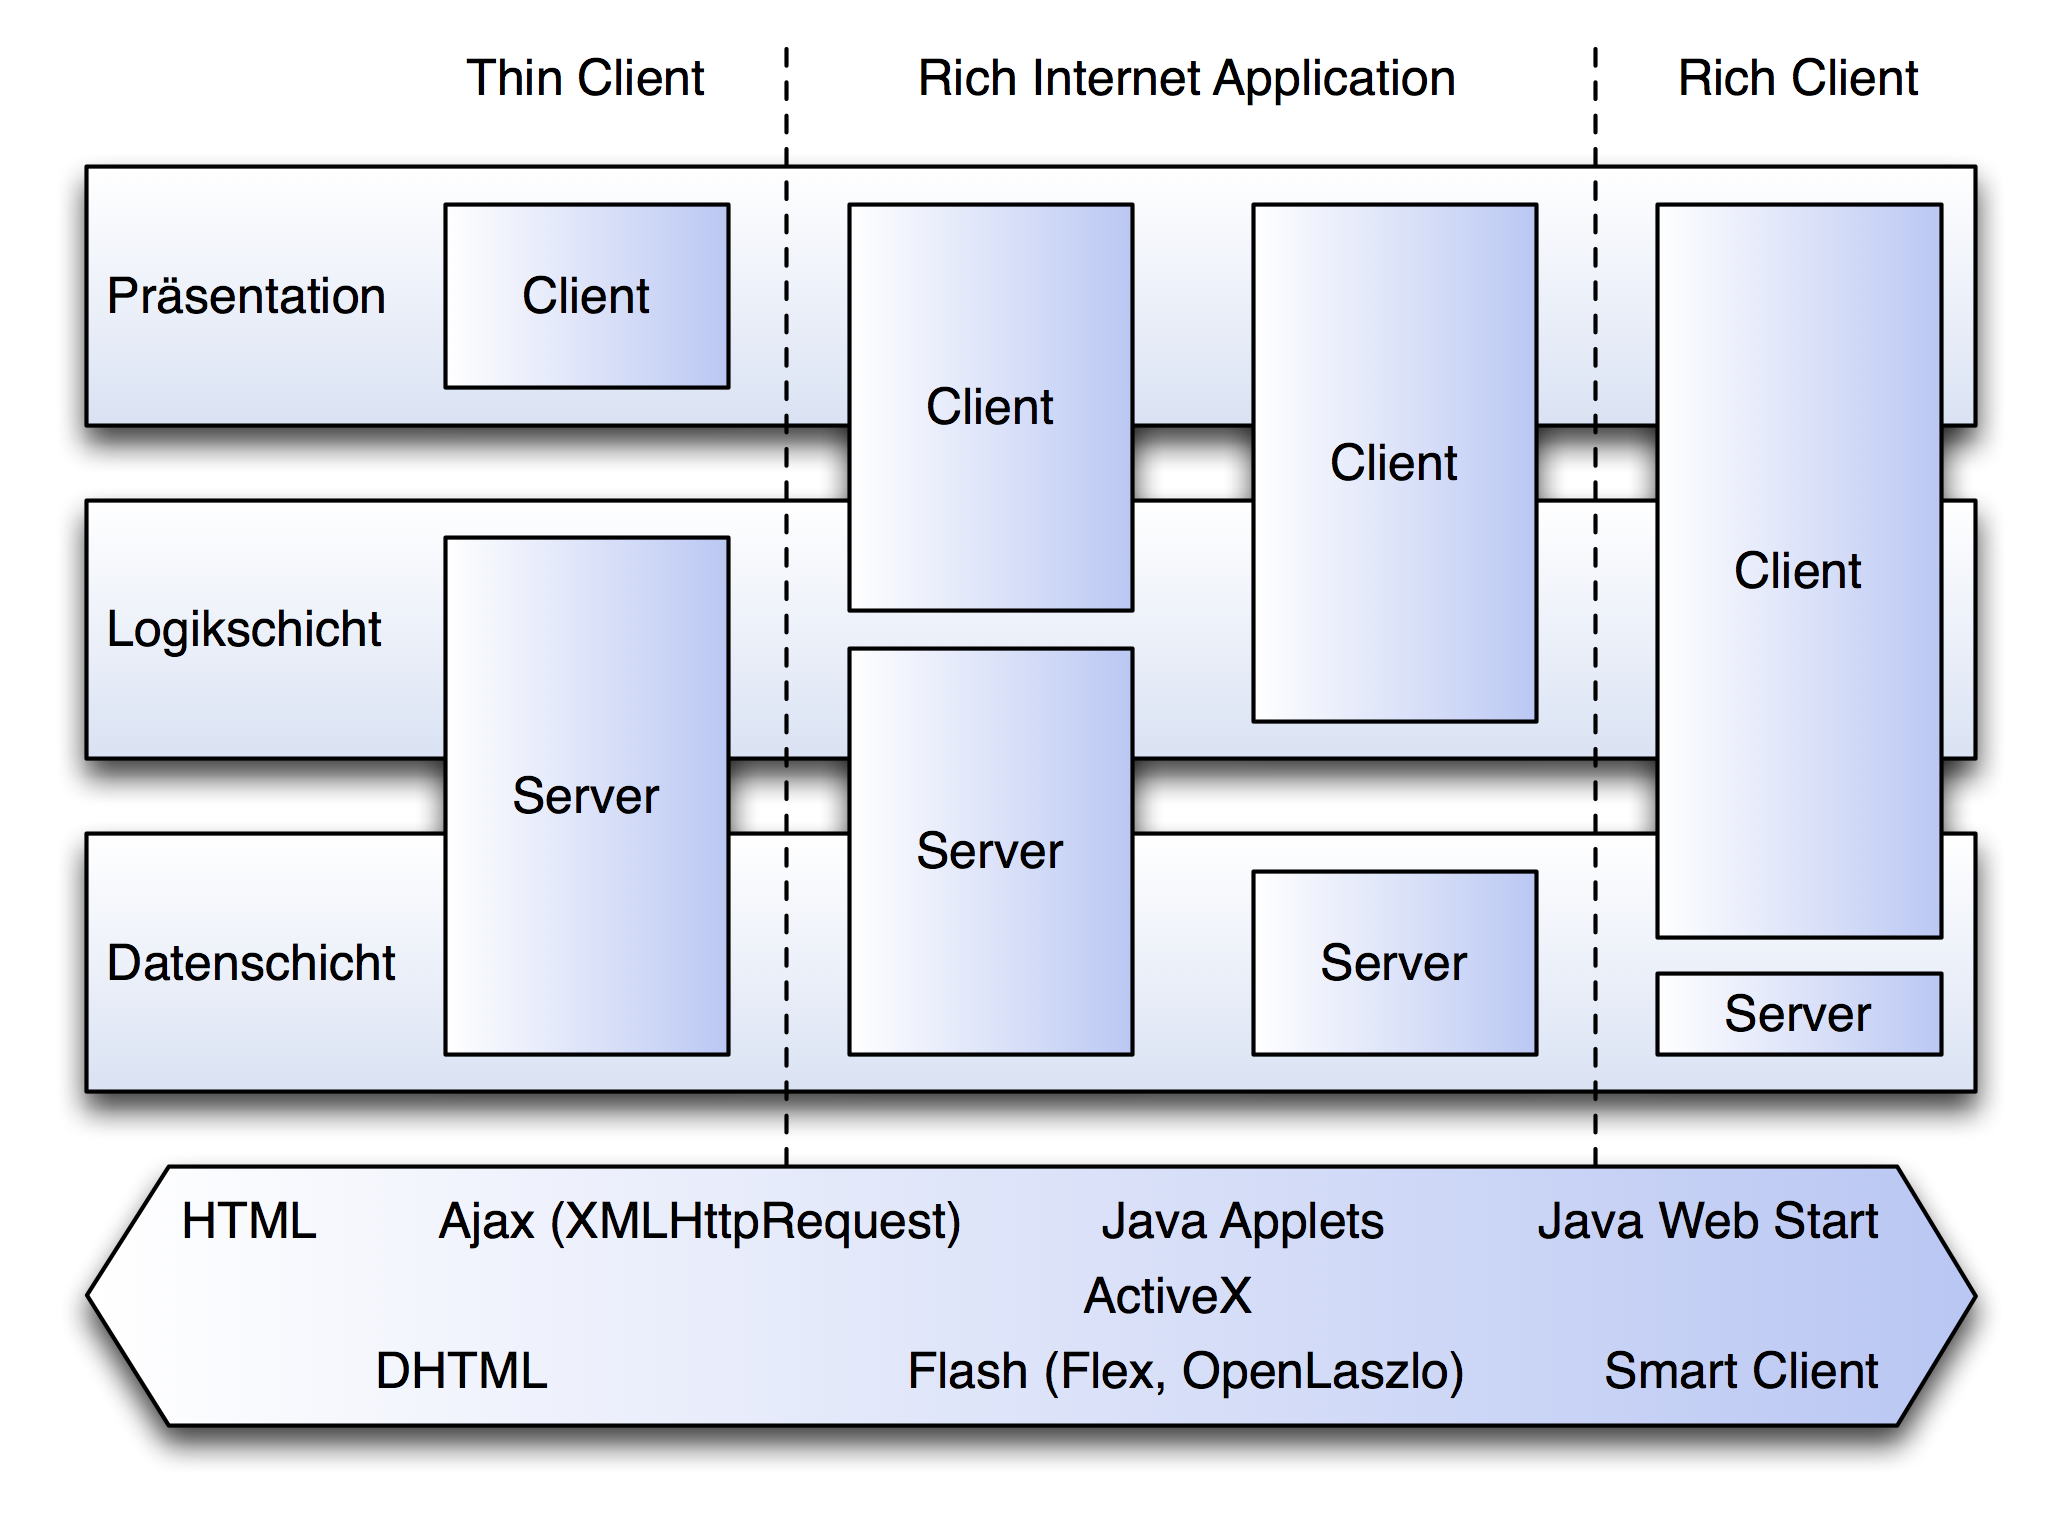
\includegraphics[width=0.85\textwidth]{./image/webanwendungen.png}
      \caption{Web Anwendungen (nach \cite{DiplomarbeitStephanSchuster} S. 6f.
      und \cite{WebApplicationSolutions} S. 5)}
      \label{img:webanwendungen}
    \end{center}
  \end{figure}
  
  Rich Client steht für kompilierte Desktopapplikationen und Thin Client für
  Webapplikationen welche im Webbrowser laufen, siehe
  \cite{WebApplicationSolutions} S. 4f. Da die Grenze zwischen \ac{RIA} und
  Thin Client nicht klar definiert ist, werden diese beiden Begriffe zum Teil
  als Synonym verwendet.
  
  \section{Klassifikation}
  
  Es wird eine Klassifikation aller \ac{RIA} in die Klassen der Plugin
  orientierten, der Client orientierten und der Browser orientierten gemacht.
  
  \subsection{Plugin orientiert}
  
  Plugin orientierte \ac{RIA} sind Applikationen, welche in einem Browser
  Plugin laufen. Dabei sind Adobe Flash, Java Applet und Microsoft Silverlight
  die drei grössten Vertreter in dieser Sparte, siehe \cite{RichInternetApplications}
  und \cite{RichInternetApplicationMarketShare}.

  \subsection{Client orientiert}
  
  Unter Client orientiert versteht man lediglich, dass alle Desktopanwendungen,
  welche entweder mit den Internet kommunizieren oder zumindes über dieses
  ausgeliefert werden, zu dieser Kategorie gehören. Dies trifft nur zu, in der
  Annahme, dass Desktopanwendungen eine ``reichhaltige'' Bedienoberfläche
  anbieten, siehe \cite{RichInternetApplication}. Eine Java Swing Applikation
  könnte also auch als Client orientierte \ac{RIA} klassifiziert werden.
  
  \subsection{Browser orientiert}
  
  Browser orientierte \ac{RIA} kommen aus der Evolution der Internettechnologie
  heraus. Da sich die Grundkonzepte der Internettechnologie in den letzten
  Jahren stark verändert haben, müssen wir zwischen klassischen Webanwendungen
  und Webanwendungen mit Ajax unterscheiden.
  
  \subsubsection{Klassische Webanwendung}
  
  Um die Jahrtausenwende wurden klassische Webanwendung nach dem Prinzip von
  Request - Response aufgebaut. Der Benutzer konnte mit einer Interaktion einen
  Statuswechsel von einer Seite zur Nächsten auslösen, zum Beispiel durch das
  anklicken eines Links oder mit dem Versenden eines HTML-Formulars, siehe
  Abbildung \ref{img:classicPageReload}. Der zeitliche Ablauf sieht mit einem
  \ac{UML} Sequenzdiagramm wie folgt aus, siehe Abbildung
  \ref{img:sequenzdiagrammClassicPageReload}. Dabei wurde immer der gesamte
  Seiteninhalt neu geladen, was zu langen wartezeiten beim Laden der Seite und
  zu einem ungewohnten Anwendergefühl, im Vergleich zu Desktopanwengungen,
  geführt hat. Zudem wurden immer alle Daten vom Server an den Browser
  übermittelt, welche für die Darstellung der Webanwendung von Nöten war, siehe
  \cite{AjaxInAction} S. 44ff.
  
  \begin{figure}[hbt]
    \begin{center}
      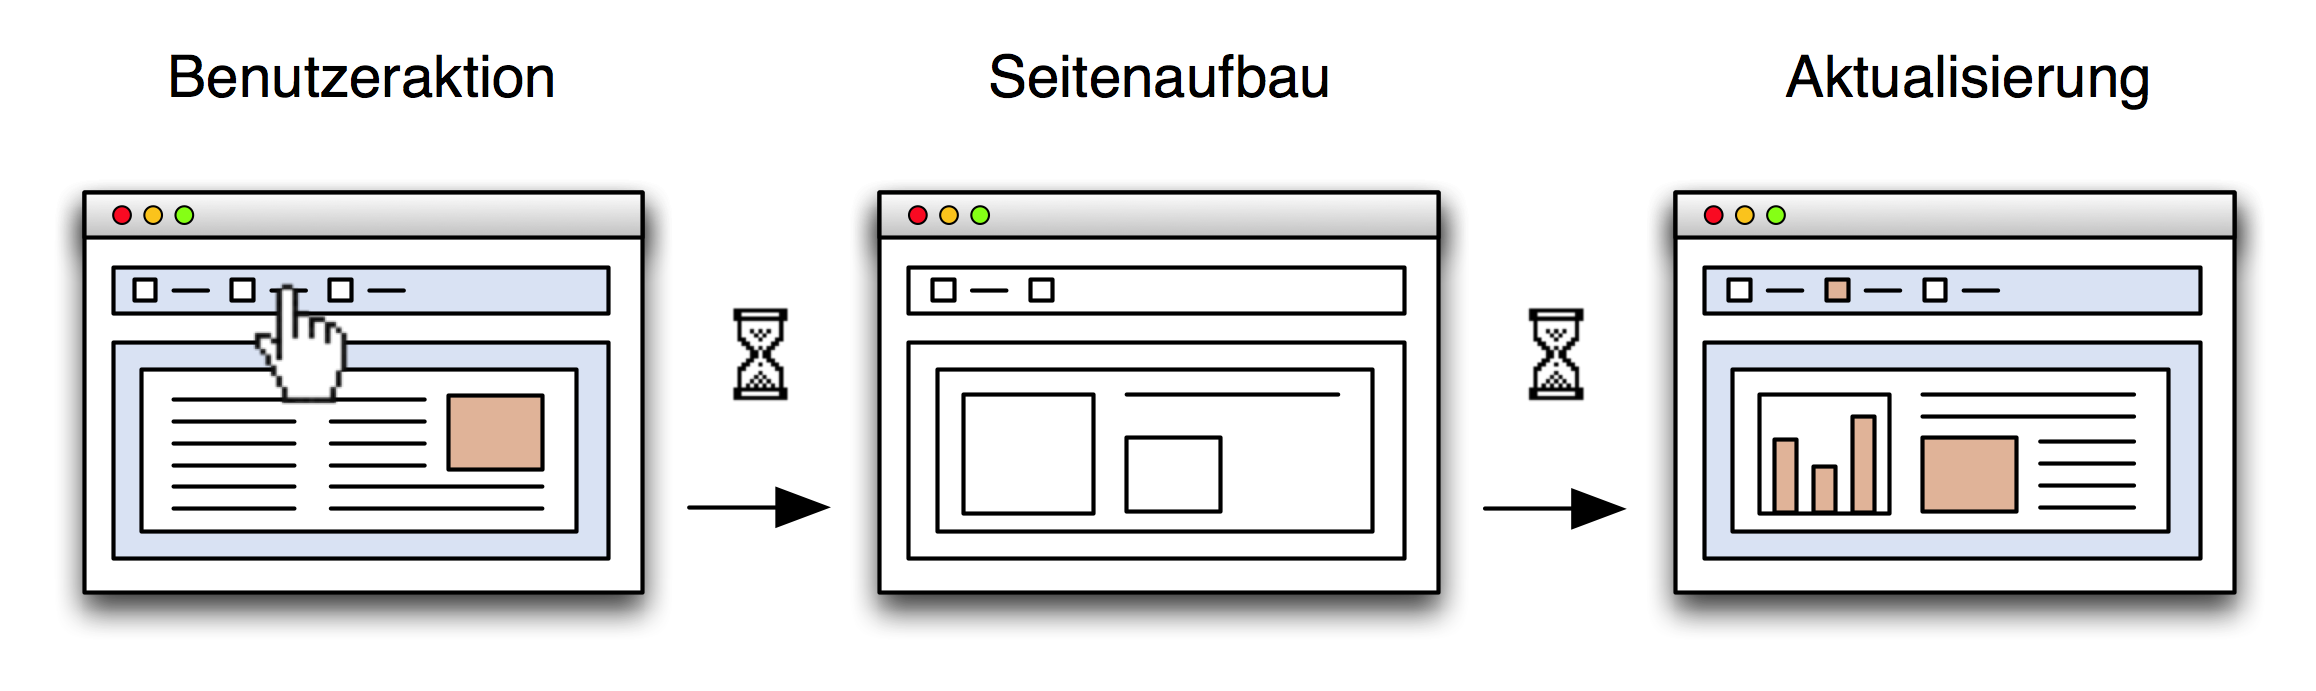
\includegraphics[width=\textwidth]{./image/classicPageReload.png}
      \caption{Klassische Webanwendung aus der Usersicht (nach
      \cite{DiplomarbeitStephanSchuster} S. 10)}
      \label{img:classicPageReload}
    \end{center}
  \end{figure}
  
  \begin{figure}[hbt]
    \begin{center}
      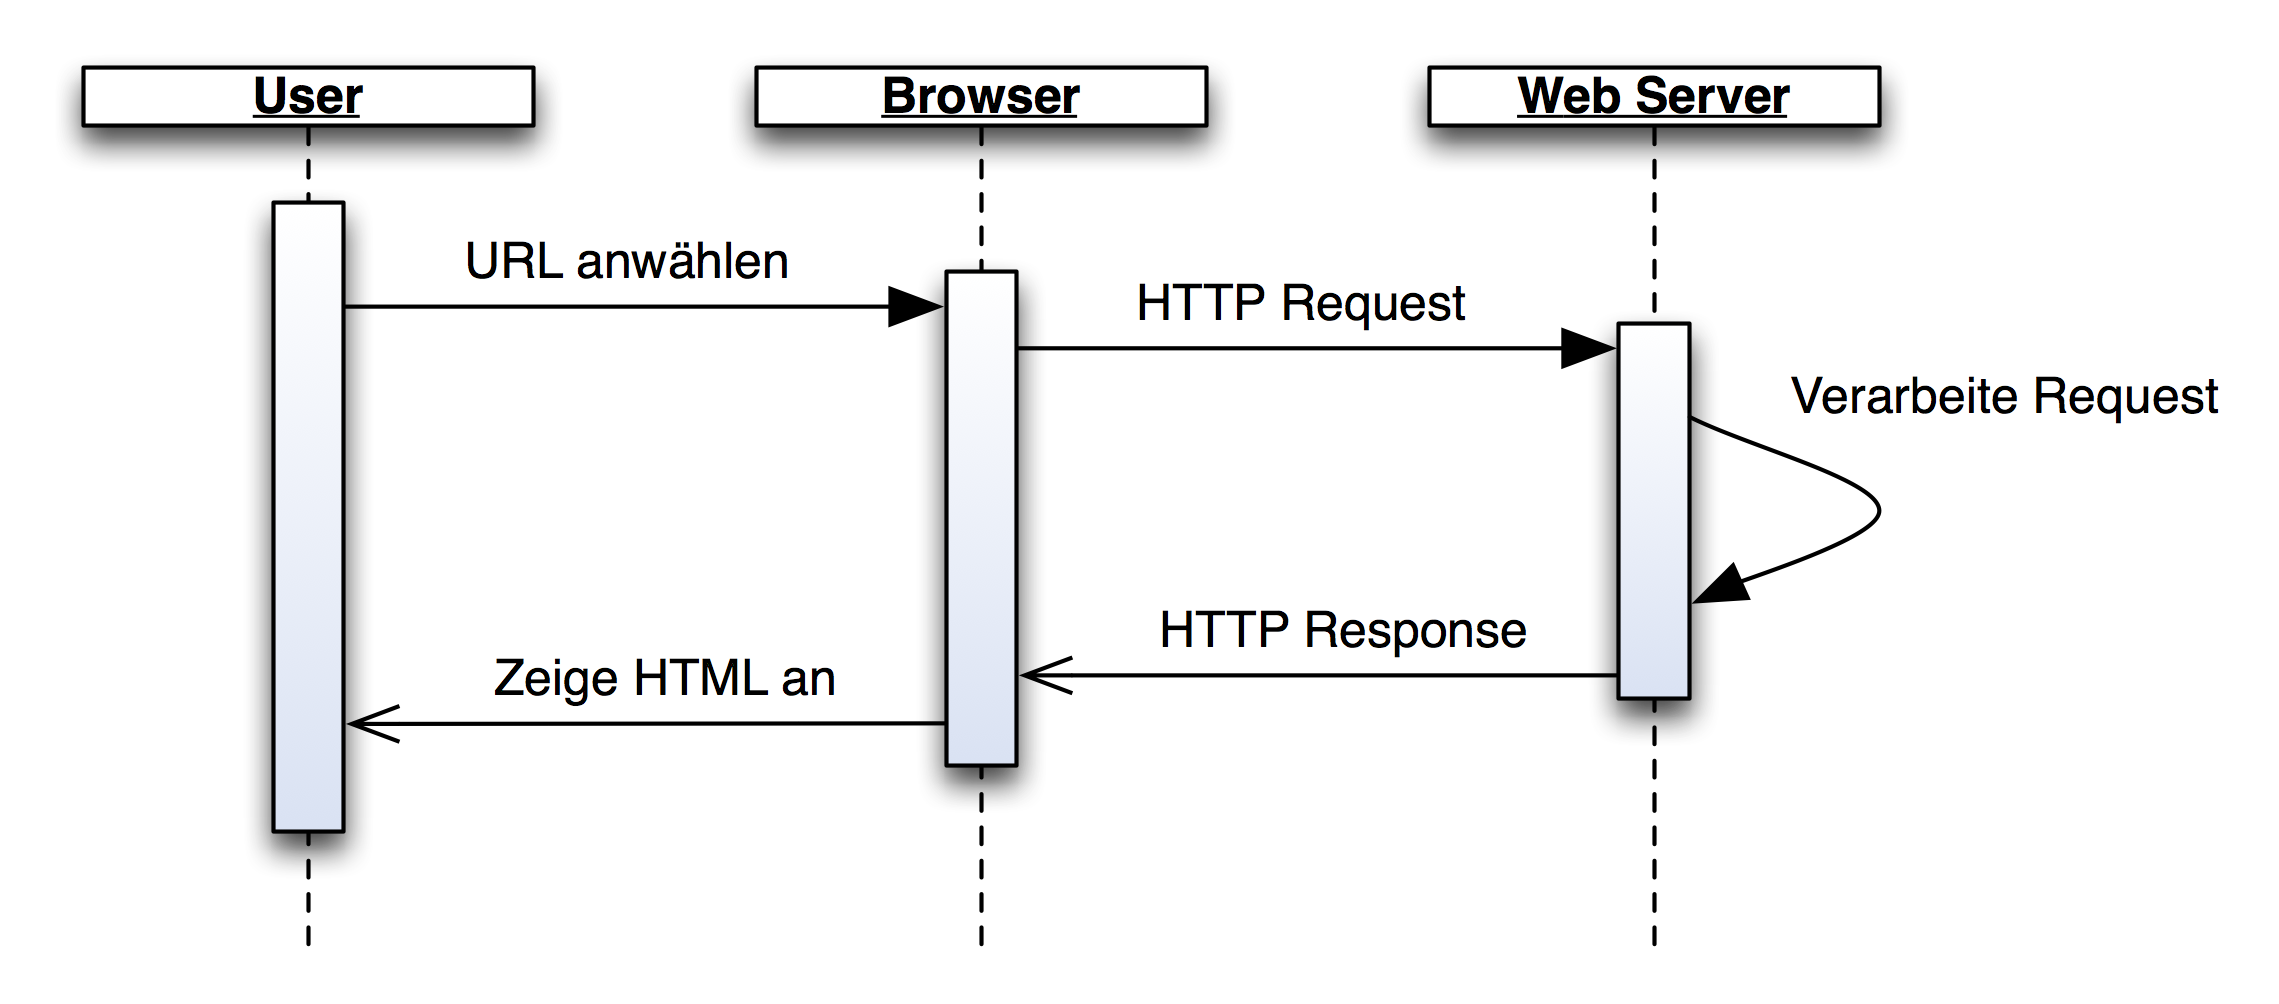
\includegraphics[width=0.85\textwidth]{./image/sequenzdiagrammClassicPageReload.png}
      \caption{HTTP Request als \ac{UML} Sequenzdiagramm (nach
      \cite{HttpBasics} S. 10)}
      \label{img:sequenzdiagrammClassicPageReload}
    \end{center}
  \end{figure}
  
  \subsubsection{Webanwendung mit Ajax}
  
  Mit dem Konzept von \ac{Ajax}, bei dem der Browser asynchron Daten vom Server
  nachladen kann, wurde die Möglichkeit geschaffen, Anwendungen zu entwickeln,
  welche sich in der Bedienung wie Desktopanwendungen anfühlen, siehe Abbildung
  \ref{img:ajaxPageReload}. Der zeitliche Ablauf sieht mit einem \ac{UML}
  Sequenzdiagramm wie folgt aus, siehe Abbildung
  \ref{img:sequenzdiagrammAjaxPageReload}. Das Prinzip funktioniert dadurch,
  dass eine zusätzliche Schicht zwischen dem Browser und Server eingerichtet
  wird. Diese Schicht, ich nenne sie hier Ajax-Engine, übernimmt die Kontrolle
  über die Datenkommunikation zum Server. Die Ajax-Engine bietet die
  Möglichkeit asynchron zur Clientinteraktion Daten vom Server anzufordern und
  bei Erhalt dynamisch in die bestehende Seite einzuflechten. Das Ergebnis ist,
  dass der Browser vom Server entkoppelt wird, wobei der Benutzer die Seite
  weiterhin verwenden kann. Der Server kann nun im Hintergrund getätigte
  Interaktionen verarbeiten.
  
  \begin{figure}[hbt]
    \begin{center}
      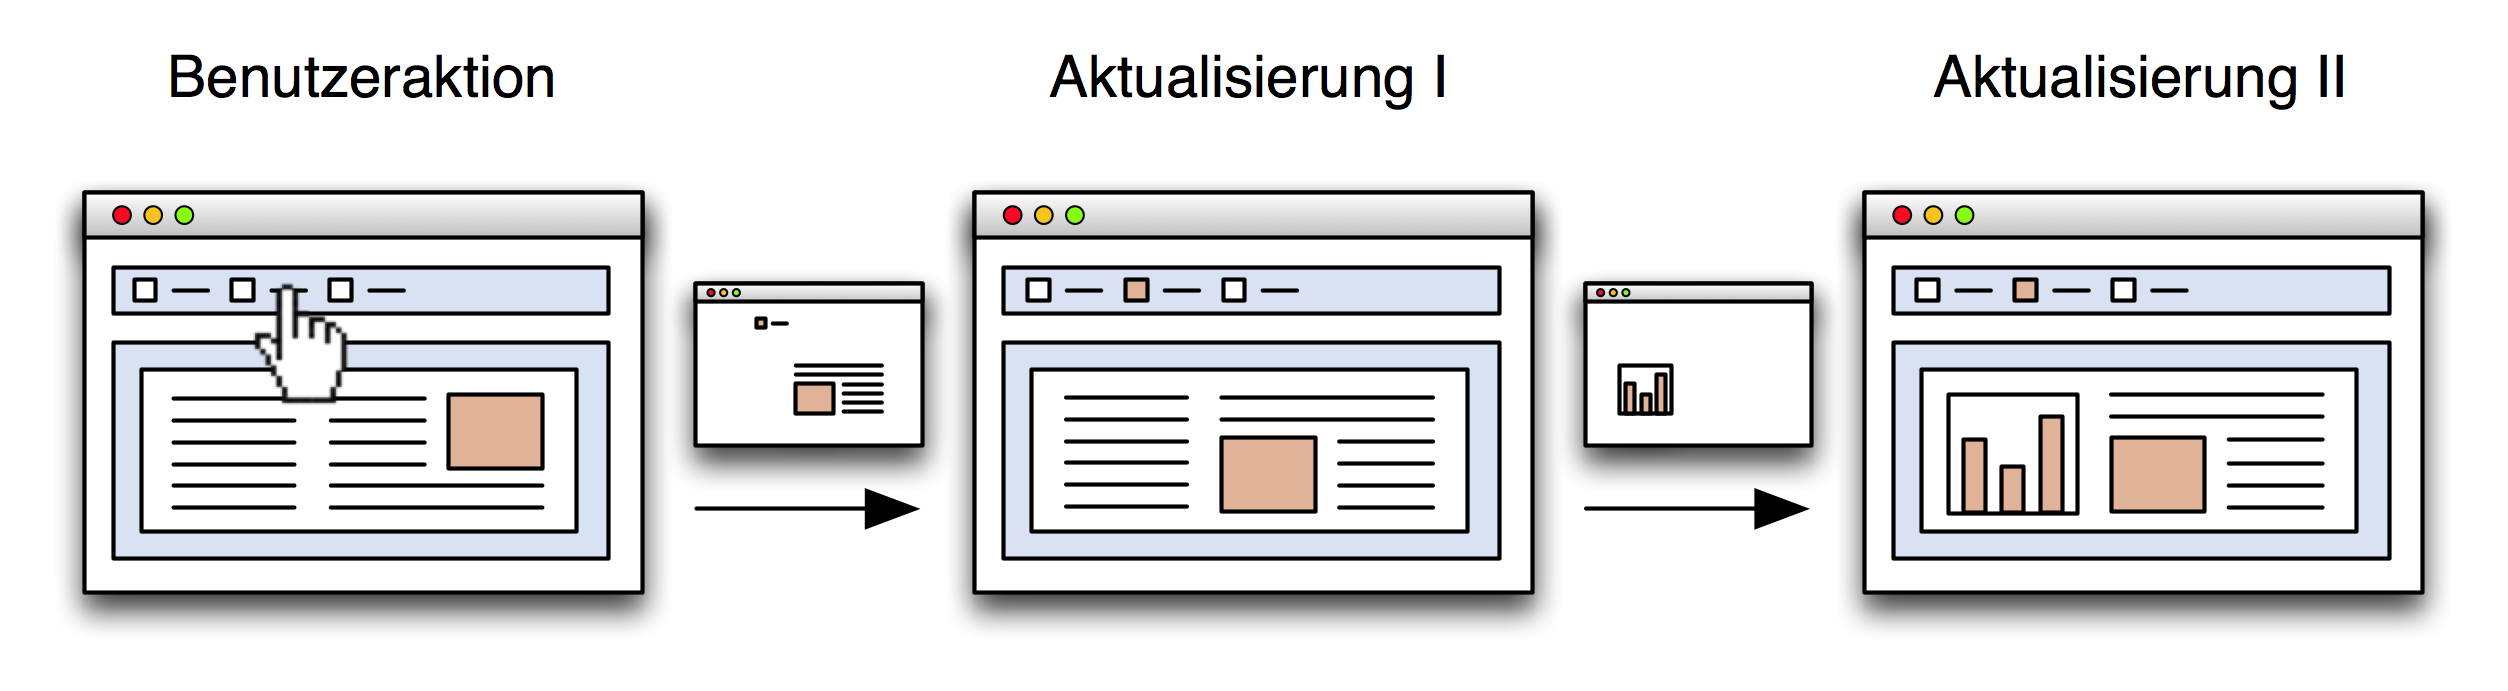
\includegraphics[width=\textwidth]{./image/ajaxPageReload.png}
      \caption{Webanwendung mit Ajax aus der Usersicht (nach
      \cite{DiplomarbeitStephanSchuster} S.12)}
      \label{img:ajaxPageReload}
    \end{center}
  \end{figure}
  
  \begin{figure}[hbt]
    \begin{center}
      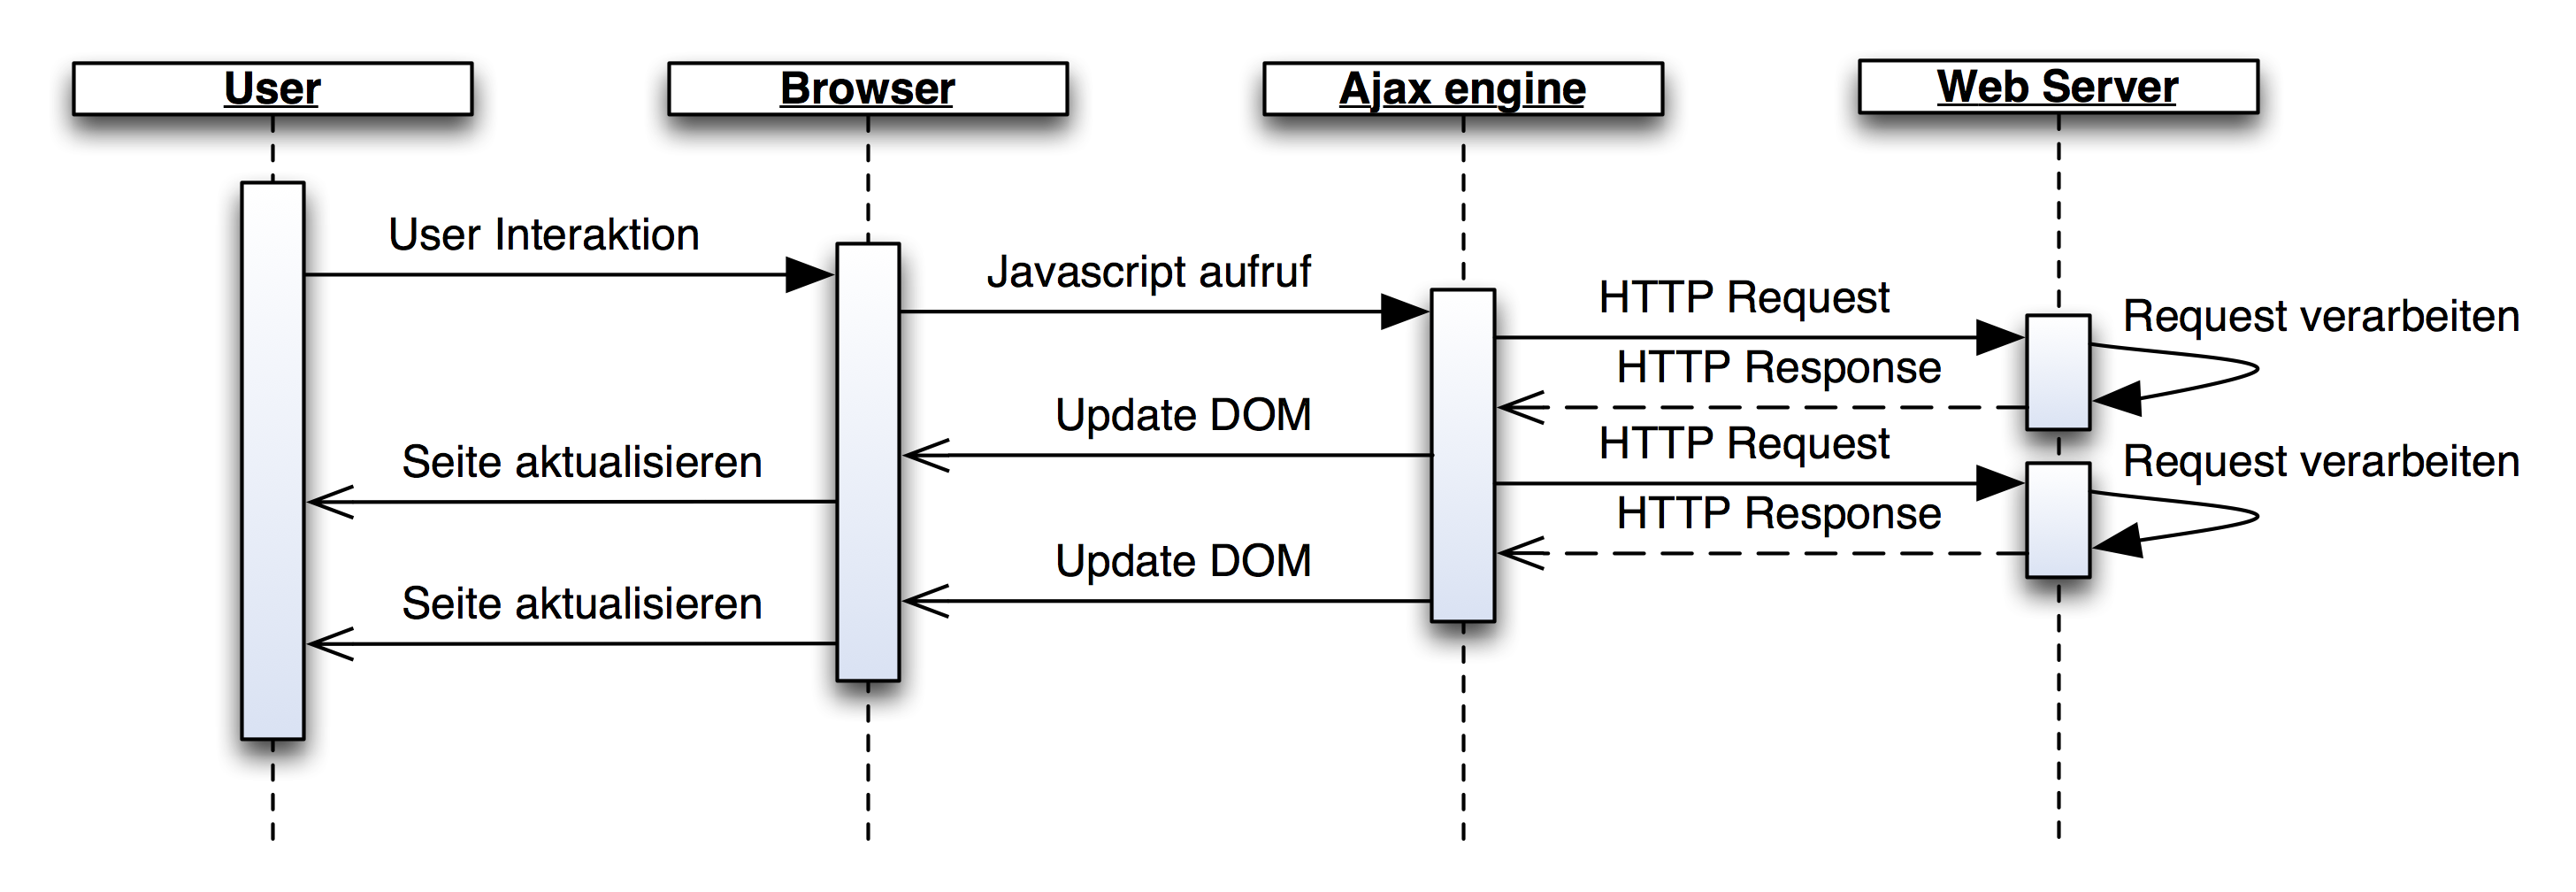
\includegraphics[width=\textwidth]{./image/sequenzdiagrammAjaxPageReload.png}
      \caption{Ajax Request als \ac{UML} Sequenzdiagramm}
      \label{img:sequenzdiagrammAjaxPageReload}
    \end{center}
  \end{figure}
  
  \subsubsection{Security}
  
  Nach \cite{RichInternetApplication} gelten Browser orientierte \ac{RIA},
  welche auf Webstandards\footnote{Webstandards werden durch das Gremium W3C
  definiert, siehe \url{http://www.w3.org/}} basieren, als relativ sicher.
  Mögliche Sicherheitslöcher stellen vorallem der jeweils verwendete Browser,
  in der die Applikation dargestellt wird, und Attacken nach dem Prizip von
  Social Engineering\footnote{Bei Social Engineering geht es darum, durch
  zwischenmenschliche Beeinflussung, unberechtigt an Daten oder Dinge zu
  gelangen, siehe \cite{SocialEngineering}}.
  
  \subsubsection{Suchmaschinenoptimierung}
  
  Suchmaschinenoptimierung dient dazu im Ranking einer Suchmaschine besser
  abzuschliessen. Dies ist vorallem bei Unternehmen von Bedeutung, welche das
  Internet als Vertriebkanal sehen. Bei statischen Webseiten ist das Indexieren
  ein Prozess der gut funktioniert. Bei einer \ac{RIA}, welche über \ac{Ajax}
  Daten zur Laufzeit einer Webapplikation asynchron nachlädt, wird das für eine
  Suchmaschine ein schwierigeres Unterfangen, die Daten Sinnvoll abzugreifen.
  
  \section{Vorgaben aus der IT-Architektur der Zürcher Kantonalbank}
  
  In der Zürcher Kantonalbank gibt es klare Vorschriften, welche Arten von
  \ac{RIA} eingesetzt werden dürfen. Diese Vorschriften werden im Handbuch der
  IT-Architektur zusammengefasst, siehe \cite{ZkbHandbuchDerItArchitektur} S.
  140ff. 
  
  \subsection{Restriktion}
  
  Aus den Vorschriften der IT-Architektur, geht hervor, dass keine neuen
  Applikationen als Plugin orientierte \acp{RIA} entwickelt werden, siehe
  \cite{ZkbHandbuchDerItArchitektur} S. 143f. Zudem wird festgelegt, dass
  Client orientierte \acp{RIA} für neue Applikationen nicht in Frage kommen,
  falls die Business-Logik im Client liegt, siehe
  \cite{ZkbHandbuchDerItArchitektur} S. 141f.
  
  \subsection{Mögliche Implementierung}
  
  Als mögliche Implementierung werden von der IT-Architektur der \ac{ZKB} zwei
  Gruppen genannt. Die Gruppe der Thin Clients und die Gruppe der Ultra Thin
  Clients. Die Gruppe der Thin Clients ist gemäss dem IT-Architektur Handbuch
  eine Java Desktop Applikation, welche nur eine Präsentations-Logik enthält.
  Die Gruppe der Ultra Thin Clients entspricht den Browser orientierten
  \ac{RIA}, siehe Abbildung \ref{img:zkbWebAnwendungen}
  
  \begin{figure}[hbt]
    \begin{center}
      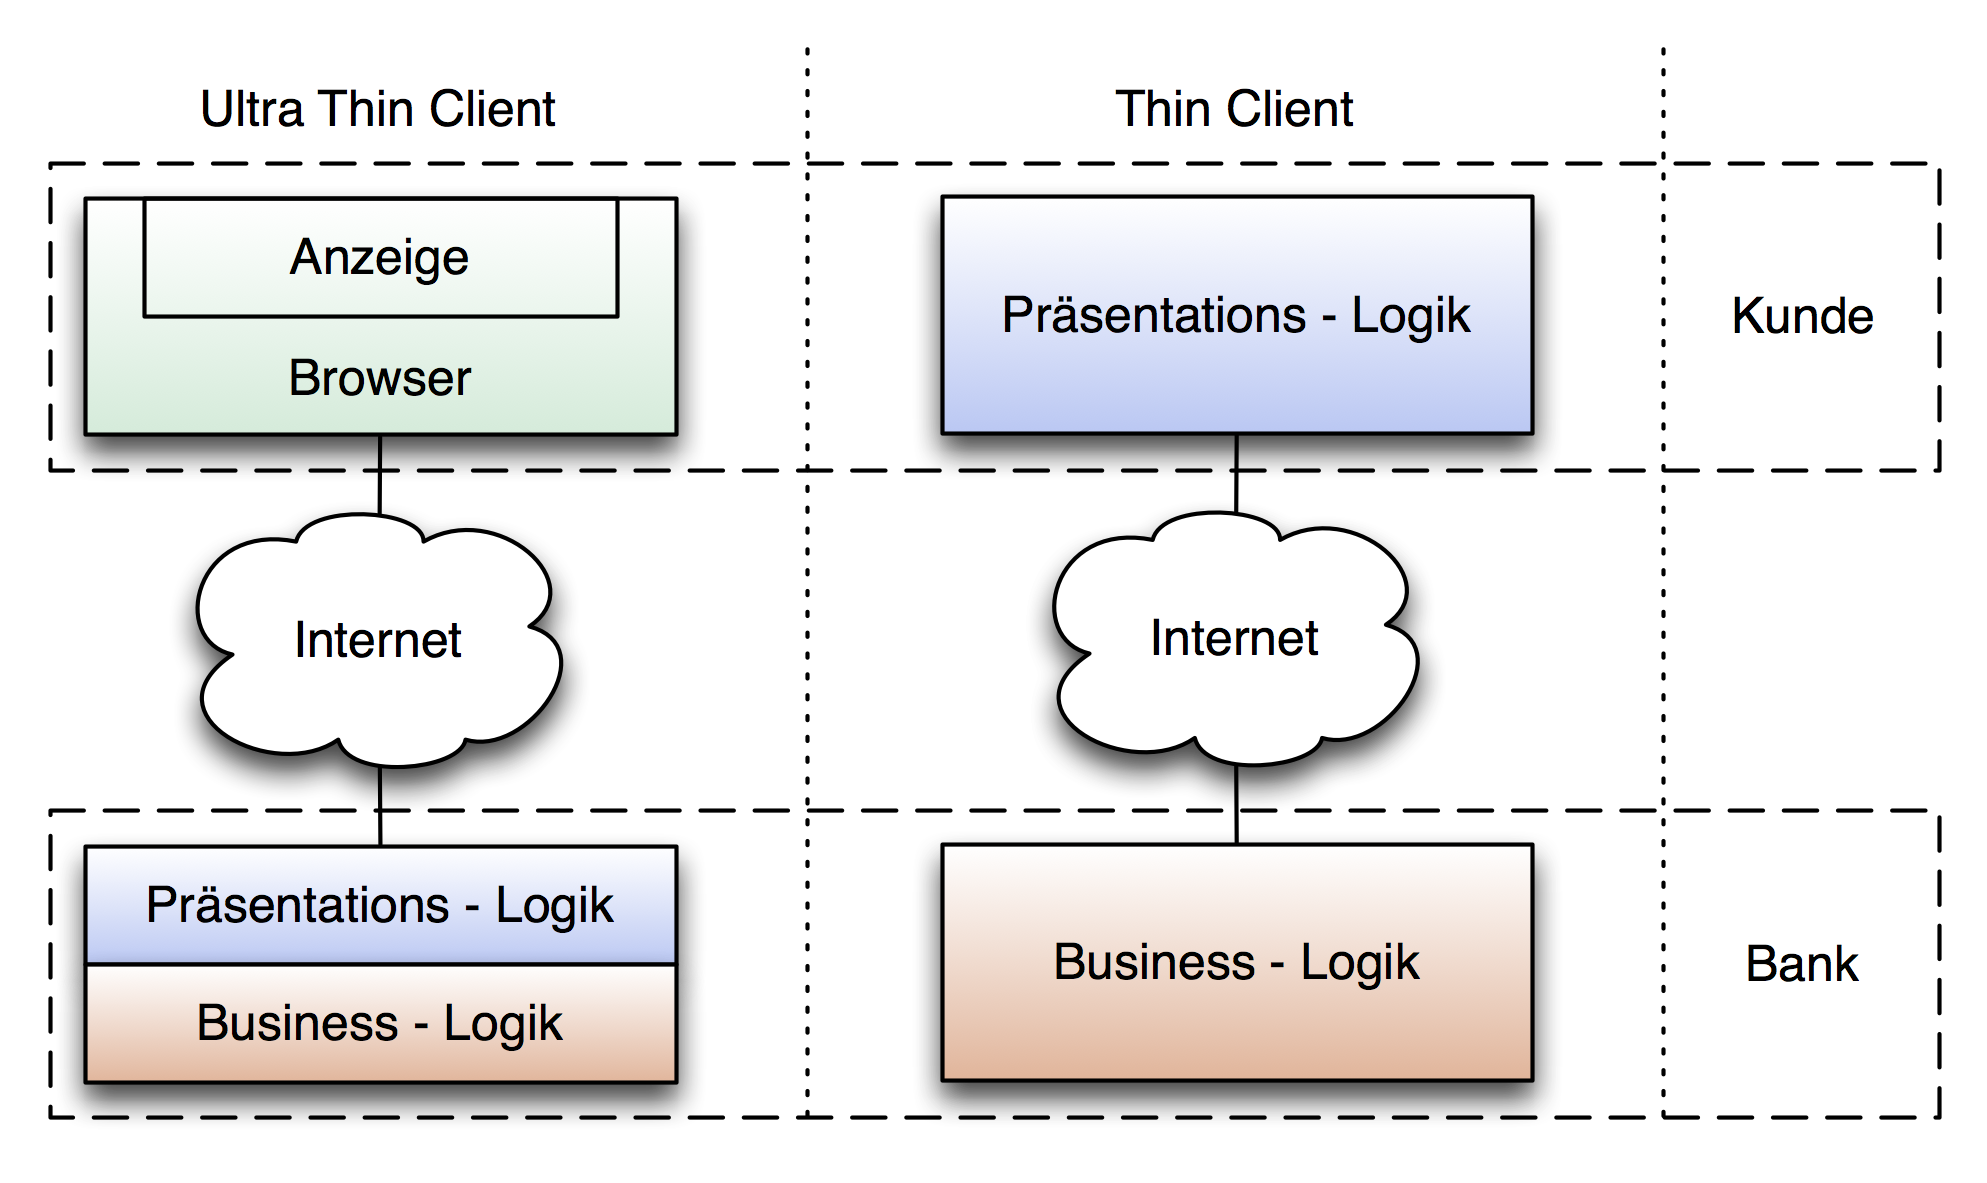
\includegraphics[width=\textwidth]{./image/zkbWebAnwendungen.png}
      \caption{Möglicher Aufbau von Web Applikationen (nach
      \cite{ZkbHandbuchDerItArchitektur} S. 141)}
      \label{img:zkbWebAnwendungen}
    \end{center}
  \end{figure}
  

  \cleardoublepage
  
  % ===========================================================================
  % Kapitel XXX beginns here
  % ===========================================================================
   
  \chapter{Infrastruktur der Zürcher
  Kantonalbank}\label{chapter:InfrastrukturDerZuercherKantonalbank}

    Im diesem Kapitel, soll auf die IT-Infrastruktur der \ac{ZKB} im Bereich der
  Web Applikationen eingegangen werden. Diese Informationen werden später dazu
  verwendet, um zu Prüfen, ob ein Java Web Framework den Ansprüchen der
  IT-Infrastruktur genügt. Die Informationen, welche hier beschrieben werden,
  stammen aus dem Handbuch der ZKB IT-Architektur, siehe
  \cite{ZkbHandbuchDerItArchitektur}. In der Abbildung
  \ref{img:infrastrukturZkb} ist die Standardkonfiguration, wie sie heute
  verwendet wird, ersichtlich.
  
  \begin{figure}[ht]
    \begin{center}
      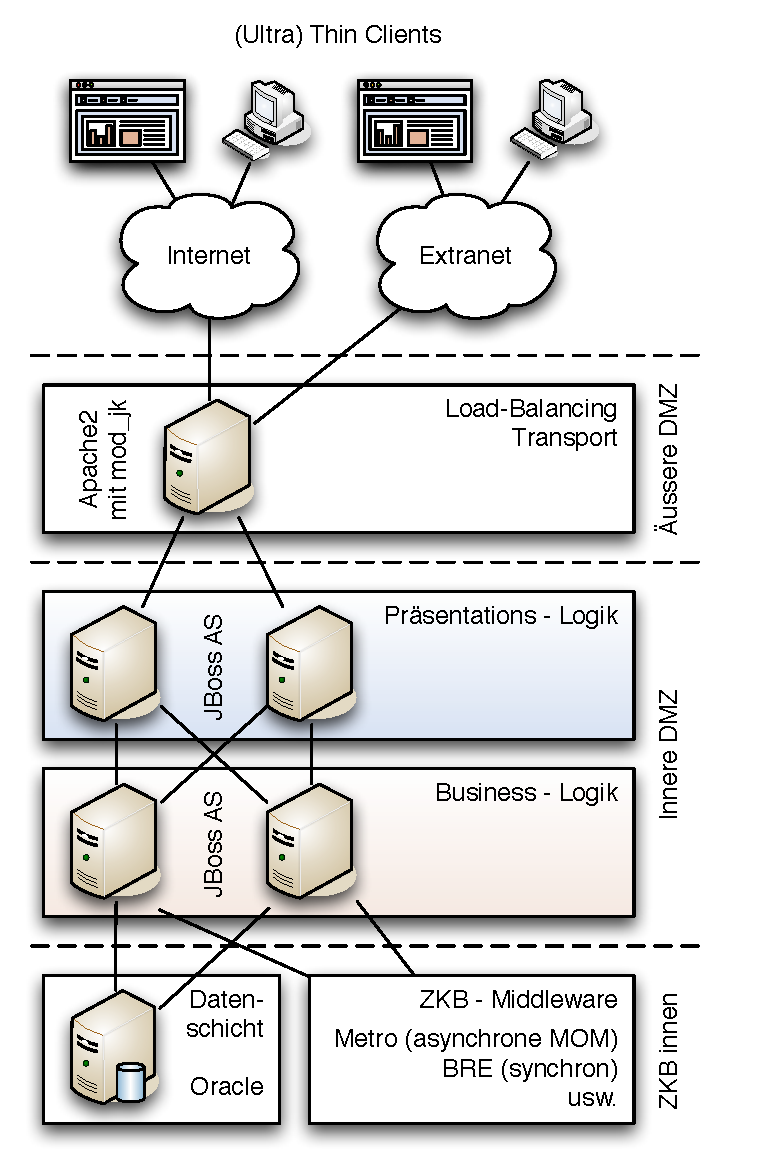
\includegraphics[width=0.87\textwidth]{./image/infrastrukturZkb.pdf}
      \caption{Architektur von Internet-Applikationen (nach
      \cite{ZkbHandbuchDerItArchitektur} S. 145)}
      \label{img:infrastrukturZkb}
    \end{center}
  \end{figure}
  
  \section{Java Runtime Environment}
  
  In allen Segmenten der Infrastruktur wird mindestens das \ac{JRE} von
  Oracle\footnote{ehemals Sun Microsystems} in der Version 1.5 zur Verfügung
  gestellt. An einigen stellen, zum Beispiel bei den Clients ist auch die
  Version 1.6 verfügbar. Diese Informationen beziehen sich auf den aktuellen
  Stand und können sich jederzeit ändern. Grundsätzlich wird nicht davon
  ausgegangen, dass ein Rückschritt in der Version vorgenommen wird, sondern
  das man gemäss der Evolution auf eine neuere Version wechselt.
  
  \section{Load-Balancing und Transport}
  
  Für das Load-Balancing und den Transport wird der Apache HTTP Server 2
  verwendet. Er gilt als anerkannter Standard und ist auf allen ZKB Plattformen
  verfügbar, siehe \cite{ZkbHandbuchDerItArchitektur} S. 146.
  
  Der Transport über \ac{HTTP} und \ac{HTTPS} gehört zu den Standardfunktionen
  des Apache HTTP Servers 2. Zudem können statische Daten direkt über den
  Apache HTTP Server 2 zur Verfügung gestellt werden, ohne das die
  Präsentations-Logik oder die Business-Logik damit belastet werden.
  
  Die Verbindung zur Präsentations-Logik und auch das Load-Balancing wird mit
  dem Modul\footnote{Der Apache HTTP Server 2 hat einen modularen Aufbau, womit
  er durch Module erweitert werden kann.} \(mod\_jk\)\footnote{Für
  Informationen zum Apache Tomcat Connector, siehe \cite{ModJk}} gemacht.
  
  \section{Präsentations-Logik}
  
  Für die Präsentations-Logik wird der Servlet/JSP Container JBoss
  Web\footnote{JBoss Web basiert auf Apache Tomcat 6.0 und implementiert die
  Standards Servlet 2.5 und JavaServer Pages 2.1, siehe \cite{JBossWeb}}
  verwendet, der ein Bestandteil des JBoss AS\footnote{JBoss AS steht für JBoss
  Application server, siehe \cite{JBossAS}} ist und auf der Open Source Software
  Apache Tomcat\footnote{Für mehr Informationen zu Apache Tomcat, siehe
  \cite{ApacheTomcat}} basiert. Der JBoss Web ist auch für die Verwaltung der
  User Sessions zuständig.
  
  Für die Präsentations-Logik wird eine komplette Instanz eines JBoss AS
  verwendet. Für die Skalierung der Web Applikation können weitere
  JBoss AS Instanzen dazugeschalten werden. In der standard Konfiguration sind
  es zwei.
  
  Für die Kommunikation zwischen der Präsentations-Logik und der Business-Logik
  werden Webservices auf der Basis von \ac{SOAP}, \ac{RMI} oder \ac{CORBA}
  verwendet. Es gibt auch eine \ac{ZKB} spezifische Lösung namens ZIP.net.
  
  Das für die Präsentations-Logik und die Business-Logik eigene JBoss AS
  Instazen verwendet werden, entspricht nicht ganz den Vorgaben, wie sie
  im Handbuch der IT-Architektur beschrieben sind, es wird aber in der Praxis
  oft so umgesetzt.
    
  \section{Business-Logik}
  
  Für die Business-Logik wird auch eine komplette Instanz eines JBoss AS
  verwendet. Für die Skalierung dieser Komponente können weitere JBoss AS
  Instanzen dazugeschalten werden. In der standard Konfiguration sind es zwei.
  
  Die Datenschicht wird über die Datenbankschnittstelle \ac{JDBC} angebunden.
  Der JBoss AS bietet für die meisten \ac{RDBMS} alles, was dafür benötigt
  wird. Es gibt auch die Konstellation, bei der ein \ac{ORM}, wie zum Beispiel
  Hibernate, verwendet wird.
  
  Die Kommunikation zwischen der Applikation und der ZKB spezifischen Middleware
  findet ebenfalls hier in der Business-Logik statt. Für die synchrone
  Kommunikation steht der \ac{BRE} zur Verfügung. Für die asynchrone
  Kommunikation gibt es Metro, was eine \ac{MOM} ist.
    
  \section{Datenschicht}
  
  Die Datenschicht wird meistens mit einem \ac{RDBMS} abgebildet. Normalerweise
  wird die Enterprise taugliche Lösung von Oracle eingesetzt. Je nach grösse
  der Applikation kann es sein, dass mehrere verschiedene \ac{RDBMS} zum Einsatz
  kommen.



  \cleardoublepage
   
  % ===========================================================================
  % Kapitel XXX beginns here
  % ===========================================================================
   
  \chapter{Methoden zur Analyse von Java Swing
  Applikationen}\label{chapter:MethodenZurAnalyseVonJavaSwingApplikationen}
  
    Dieses Kapitel zeigt Methoden zur Analyse von Java Swing Applikationen.
  Dabei wird auf statische und dynamische Programmanalyse und das Problem bei
  der Verwendung von Bibliotheken eingegangen. Es existieren wahrscheinlich
  noch weitere Ansätze, welche hier nicht behandelt werden.
  
  \section{Grundlagen}
  
  Zur Analyse von bestehender Software gibt es verschiedene Ansätze. Aus dem
  Bereich der Qualitätssicherung kommt die Technik der statischen oder
  dynamischen Programmanalyse, siehe \cite{SoftwareanalyseBegriffeUndTechniken}
  S. 5. Die dynamische Programmanalyse wird darin unterteilt in White-Box-
  und Black-Box-Tests, siehe Abbildung \ref{img:programmanalyse}. In meiner
  Arbeit werde diese Methoden zur Analyse von Elementen der grafischen
  Benutzeroberfläche einsetzten.
  
  \begin{figure}[ht]
    \begin{center}
      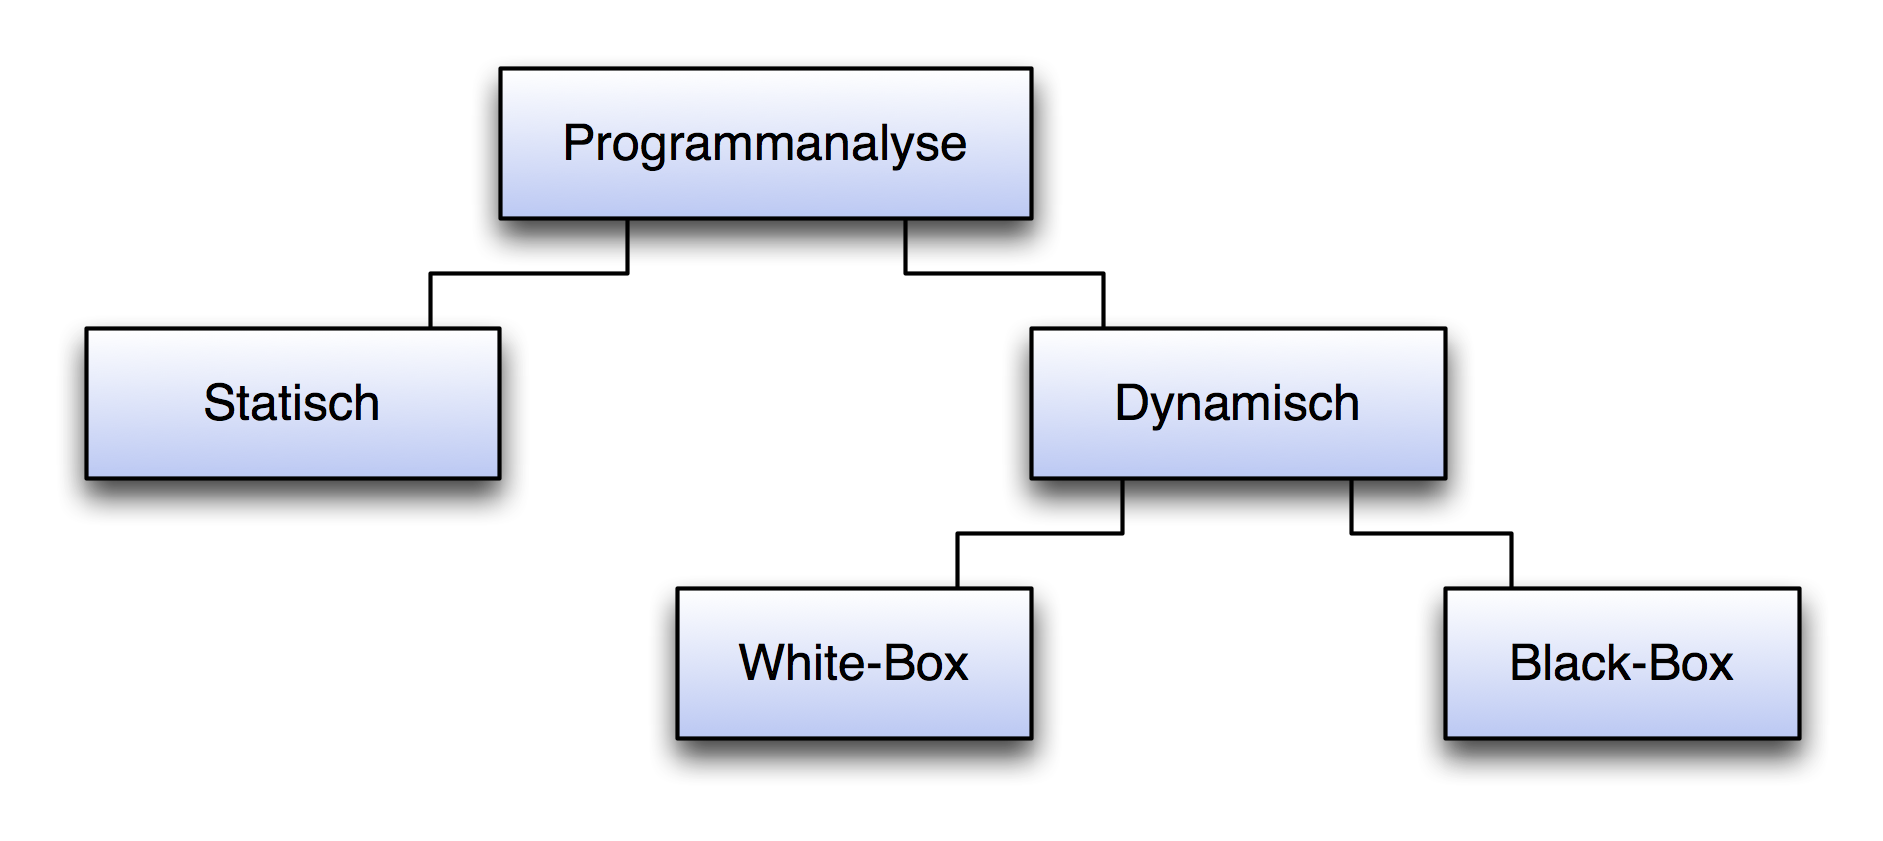
\includegraphics[width=0.6\textwidth]{./image/programmanalyse.png}
      \caption{Überblick über konventionelle Testmethoden (nach
      \cite{SoftwareanalyseBegriffeUndTechniken} S. 5)}
      \label{img:programmanalyse}
    \end{center}
  \end{figure}
  
  \subsection{Statische Programmanalyse}

  Die statische Programmanalyse basiert auf der Analyse des Sourcecodes. Das
  bedingt, dass der Sourcecode zugänglich ist. Als Softwareentwickler, kennt
  man das Verfahren eventuell aus der integrierten Entwicklungsumbegung
  (\acs{IDE})\acused{IDE}. Es gibt \acp{IDE}, wie zum Beispiel IntelliJ, siehe
  \cite{StaticCodeAnalysisIntelliJ}, die das Verfahren der statischen
  Programmanalyse nutzen. Wenn man Code schreibt, dann analysieren die
  \acp{IDE} den geschriebenen Code auf dessen syntaktische, semantische und
  lexikalische Informationen, siehe
  \cite{SoftwareQualitaetsmanagementInDerPraxis} S. 216f.
  
  Im Artikel \cite{GUIAnalysenUndBibliotheken} befasst sich der Author damit,
  was man bei \ac{GUI} lastiger Software durch eine statische Programmanaylse in
  Erfahrung bringen kann. Nach Aussage des Authors kann man bei deren
  Vorgeschlagenen Techniken folgendes erreichen:
  
  ``\begin{itshape}Im Rahmen dieser Analyse wird erkannt, welche Teile des
  Programms zur GUI gehören, welche Widgets das Programm enthält, welche
  Attribute, mit ihren Werten, diese Widgets besitzen, wie diese Widgets mit
  Events untereinander verbunden sind und wie sie in den einzelnen Fenstern der
  GUI strukturiert
  sind.\end{itshape}''\footnote{\cite{GUIAnalysenUndBibliotheken}
  Zusammenfassung - Seite 1}
    
  \subsection{Dynamische Programmanalyse}
  
  Bei der dynamischen Programmanalyse wird das zu analysierende Programm 
  ausgeführt. Die dynamische Programmanalyse wird in zwei Unterarten aufgeteilt,
  das Black-Box Verfahren und das White-Box Verfahren.
    
  \subsubsection{Black-Box Verfahren}
  
  Der Analyst hat keinerlei Informationen über das Innenleben des zu
  analysierenden Programms. Die Analyse basiert auf der intuitiven Bedienung der
  grafischen Oberfläche, durch den Analysten.
  
  \subsubsection{White-Box Verfahren}
  
  Der Analyst hat explizite Kenntnisse über das Innenleben des zu
  analysierenden Programms, zudem steht ihm der Sourcecode zur Verfügung. Mit
  der Hilfe des Sourcecodes können sinnvolle Schlüsse im Bezug auf die Analyse
  getroffen werden, da Spezialfälle, welche nicht offensichtlich sind,
  analysiert werden können. Als Beispiel dafür, möchte ich eine kurze
  Codesequenz zeigen, siehe Listing \ref{lst:dreifacherMausklick} Zeile 4.
  Dabei wird auf einen dreifachen Mausklick abgefragt. Da ein solches Verhalten nicht
  intuitiv ist, würde das ohne Sourcecode wahrscheinlich nicht gefunden werden.:
  \newline
  %\newpage
  
  \begin{lstlisting}[
    captionpos=b,
    caption=Spezialfall - dreifacher Mausklick,
    label=lst:dreifacherMausklick
  ]
  component.addMouseListener(new MouseAdapter() {
    public void mouseClicked(MouseEvent evt) {
      if (evt.getClickCount() == 3) {
        System.out.println("triple-click");
      }
    }
  });
  \end{lstlisting}
  
  \subsection{Probleme bei der Verwendung von Bibliotheken}
  
  Gemäss \cite{GUIAnalysenUndBibliotheken} S. 1f. besteht ebenfalls ein Problem
  bei der Verwendung von Bibliotheken. Die Grundproblematik besteht darin,
  dass eine Bibliothek eventuell ohne Zugriff auf deren Sourcecode verwendet
  wird. Damit wird das Verfahren der statischen Programmanalyse und der
  dynamischen White-Box Programmanalyse unmöglich.
  
  Falls eine statische Programmanalyse angestrebt wird, und der Sourcecode der
  verwendeten Bibliotheken vorhanden ist, kann sich das negativ auf die
  Präzision der Analyse auswirken. Denn es ist üblich, dass Bibliotheken
  meisst um ein Vielfaches grösser sind als das zu analysierende Programm. Der
  Aufwand wird durch die grössere Menge an Sourcecode zudem erhöht.
  
  \section{Wahl des Verfahrens}
  
  Die Wahl des Verfahrens der Analyse soll wie in der Abbildung
  \ref{img:guiAnalyse} durchgeführt werden. Leider wurde während der
  Durchführung der Diplomarbeit kein sinnvoll einsetzbares Werkzeug zur
  statischen Programmanalyse für Java Swing Applikationen gefunden. Somit wurde
  im Falle von vorhandenem Quellcode nur das dynamische White-Box Verfahren
  angewendet.
  
  \begin{figure}[ht]
    \begin{center}
      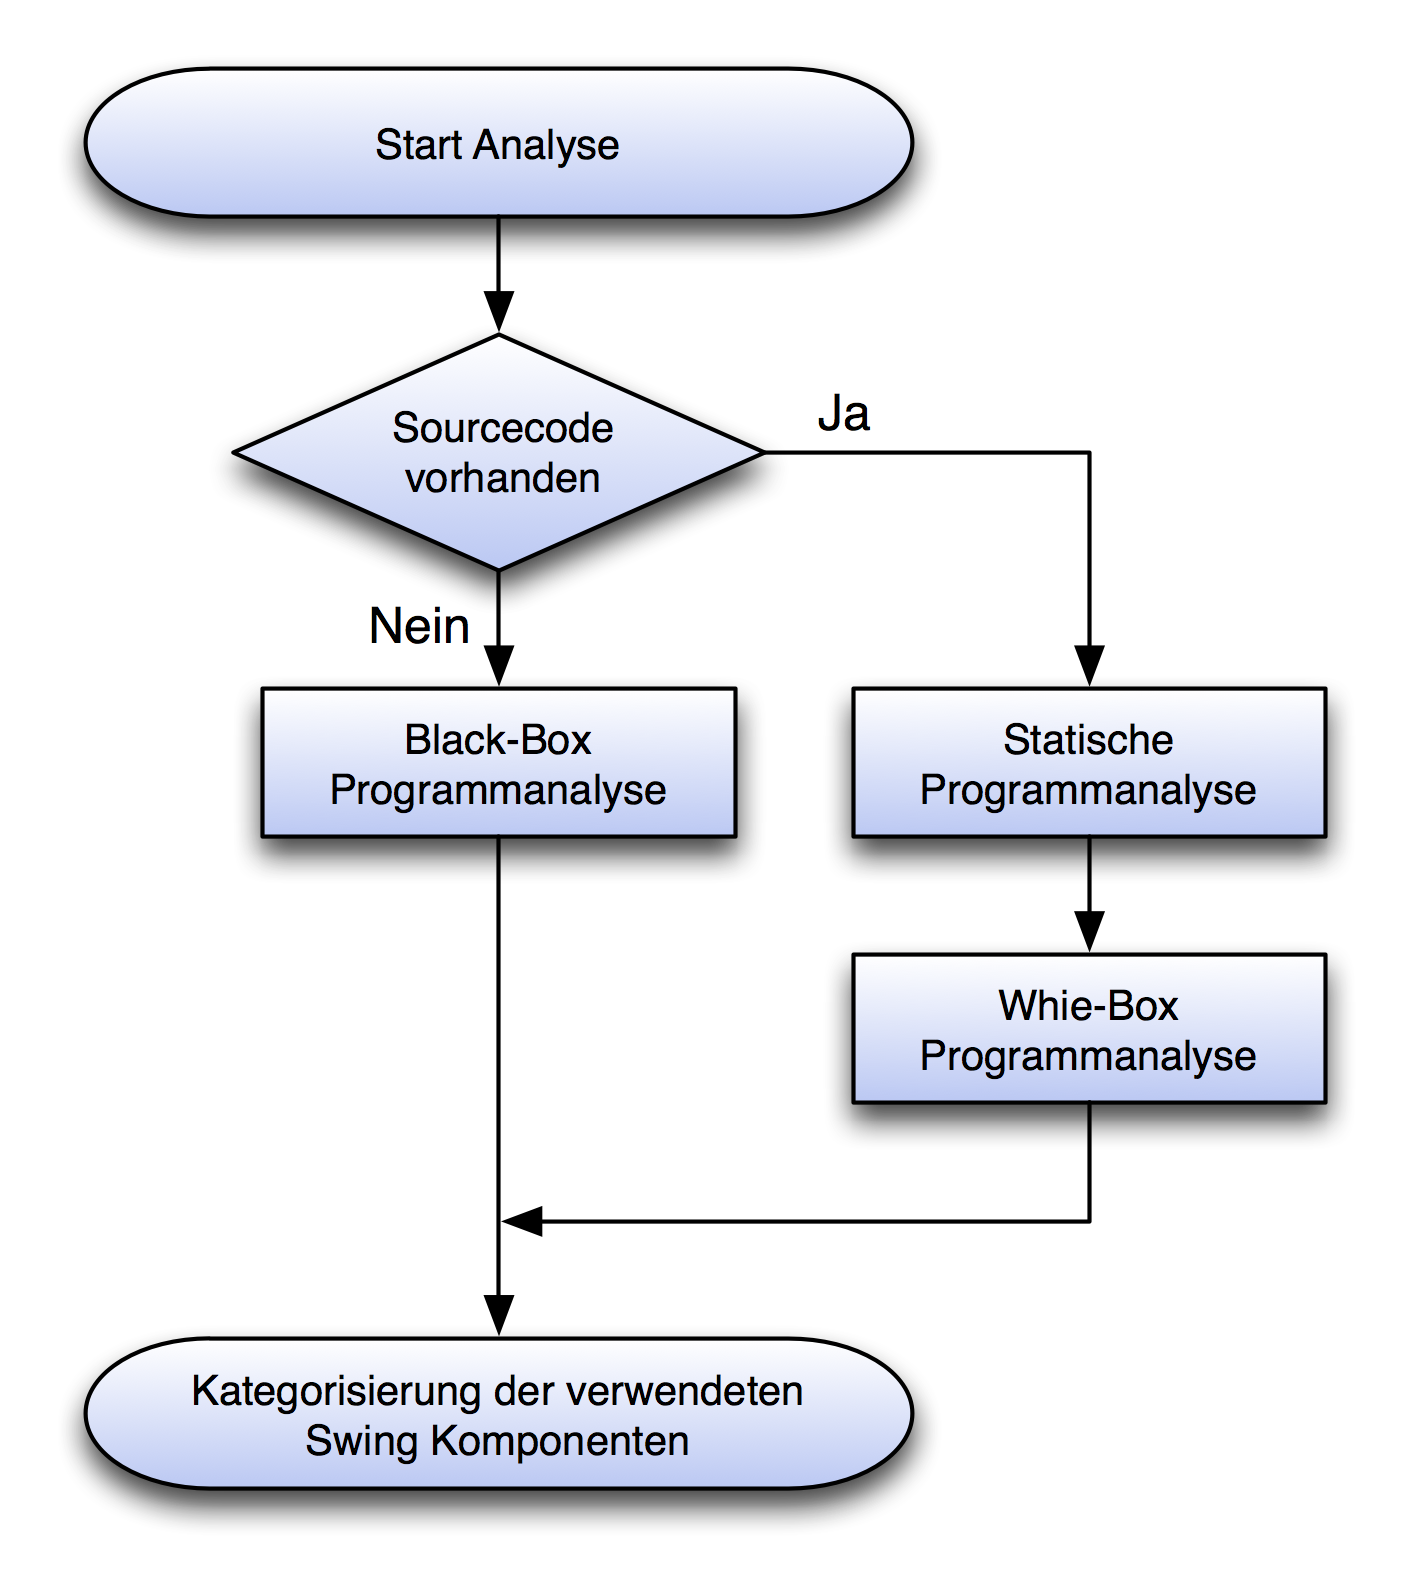
\includegraphics[width=0.5\textwidth]{./image/guiAnalyse.png}
      \caption{Wahl des Verfahrens der Programmanalyse}
      \label{img:guiAnalyse}
    \end{center}
  \end{figure}

  \cleardoublepage
  
  % ===========================================================================
  % Kapitel XXX beginns here
  % ===========================================================================
   
  \chapter{Methoden zur Entscheidungsfindung bei einer
  Evaluation}\label{chapter:MethodenZurEntscheidungsfindungBeiEinerEvaluation}
  
    Dieses Kapitel zeigt Methoden zur Entscheidungsfindung bei einer Evaluation
  auf. Dabei werden die Methoden der gewichteten Nutzwertanalyse und des
  \ac{AHP} gezeigt. Es existieren wahrscheinlich noch weitere Ansätze, welche
  hier nicht behandelt werden.
  
  \section{Grundlagen}
  
  Es gibt verschiedene Methoden wie man bei der Auswahl einer Softwarelösung
  vorgehen kann. Um eine möglichst objektive Betrachtung zu gewährleisten, wurde
  die Methode der gewichteten \ac{NWA} gewählt, siehe \cite{Nutzwertanalyse}.
  Diese Methode stammt aus dem Bereich der quantitativen Analysemethoden der
  Eintscheidungstheorie. Um eine möglichst präzise objektive Gewichtung der
  einzelnen Faktoren zu erhalten wurde dafür die Methode \ac{AHP} gewählt,
  siehe \cite{AnalyticHierarchyProcess}. Diese Methode stammt aus dem Bereich
  der präskriptiven Entscheidungstheorie. Der \ac{AHP} wurde von Thomas L.
  Saaty in den 70er Jahren des 20. Jahrhunderts entwickelt und im Buch ``The
  Analytic Hierarchy Process: Planning, Priority Setting, Resource
  Allocation'', siehe \cite{AnalyticHierarchyProcessBook}, veröffentlicht.
  
  \section{Gewichtete Nutzwertanalyse}
  
  Bei der gewichteten \ac{NWA} wird eine Menge von Alternativen \(\{A1, A2,
  A3, \ldots\}\), auf deren Nutzen, miteinander verglichen.
  
  Als Rahmenbedingung für die Durchführung der Nutzwertanalyse werden \(m\)
  KO-Kriterien \(\{KO_1, KO_2, KO_3, \ldots, KO_m\}\) bestimmt. Ein
  KO-Kriterium wird definiert durch die Erfüllung einer Bedingung. Wenn die Bedingung
  zutrifft, führt das zum KO\footnote{Der Begriff KO steht für Knock-Out und
  stammt aus der Boxwelt. Im falle einer Nutzwertanalyse bedeutet es, dass die
  Alternative aus der Nutzwertanalyse ausgeschlossen wird.} einer darauf
  geprüften Alternative.
  
  Für den Vergleich der Alternativen werden \(n\) vergleichbare
  Soll-Kriterien, auch Anforderungen genannt, definiert \(\{Soll_1, Soll_2,
  Soll_3, \ldots, Soll_n\}\). Jedes Soll-Kriterium wird durch einen
  Gewichtungsfaktor \(g_i\) versehen, was die Präferenz des Soll-Kriteriums
  wiederspiegelt. 

  Die Gewichte \(g_i\) werden so gewählt, dass ihre Summe 1.0 (100\%) ergibt,
  siehe Formel \ref{eq:gewicht}.
  
  Für jede zu evaluierende Alternative soll nun geprüft werden, ob eines
  der KO-Kriterien erfüllt ist, was zu einem Ausschluss der Alternative führen
  würde, siehe Abbildung \ref{img:rahmenbedingungenPruefen}.
  
  Falls das nicht für alle Alternativen der Fall ist, wird ein Vergleich der
  im Rennen bleibenden Alternativen über die definierten Soll-Kriterien
  geführt. Dabei werden für jede Alternative die einzelnen Soll-Kriterien mit
  einem Erfüllungsgrad \(e_i\) bewertet. Die Skala der Erfüllungsgrade ist in
  der Tabelle \ref{tab:erfuellungsgrade} ersichtlich.
  
  Der Nutzwert einer Alternative ergibt sich durch die Formel \ref{eq:nutzwert}.
  \newline
  
  \begin{table}[hbt]
    \sffamily 
    \begin{center}
      \begin{tabular}{lc}
        \toprule
        \textbf{Erfüllungsgrad} & \textbf{Skala}\\
        \midrule
        nicht erfüllt & 0\\
        schlecht & 1, 2\\
        mittel & 3 - 5\\
        gut & 6 - 8\\
        sehr gut & 9\\
        \bottomrule
      \end{tabular}
      \caption{Skala der Erfüllungsgrade}
      \label{tab:erfuellungsgrade}
    \end{center}
  \end{table}
  
  Diejenige Alternative mit dem grössten Nutzwert entspricht am meisten den
  Anforderungen. Wie gut eine Alternative nun den gestellten Anforderungen
  entspricht, kann anhand ihres berechneten Nutzwertes in der Tabelle
  \ref{tab:erfuellungsgrade} abgelesen werden.

  \begin{equation}
    \label{eq:gewicht}
    Gewicht := \sum \limits_{i=1}^n g_i = 1.0
  \end{equation}
  
  \begin{equation}
    \label{eq:nutzwert}
    Nutzwert := \sum \limits_{i=1}^n e_i \cdot g_i
  \end{equation}
  
  \subsection{Anschauliches Beispiel}
  
  Als anschauliches Beispiel sollen zwei Alternativen - Auto \(A1\) und Auto
  \(A2\) - miteinander auf die Soll-Kriterien - Leistung, Aussehen und
  Alltagstaublichkeit - verglichen werden. Es wurden keine KO-Kriterien
  definiert. In der Tabelle \ref{tab:beispielNwa} ist ersichtlich, dass das
  Auto \(A1\) dem Auto \(A2\) gegenüber bevorzugt werden soll, da der Nutzwert
  von \(A1\) (5.0) grösser ist als der Nutzwert von \(A2\) (4.7).
  \newline
  
  \begin{table}[h!]
    \sffamily 
    \begin{center}
      \begin{tabular}{lrrrrr}
        \toprule
        \textbf{Kriterien} & \textbf{Gewichtung \(g\)} & \textbf{\(e_{A1}\)} &
        \textbf{Wertigkeit \(A1\)} & \textbf{\(e_{A2}\)} & \textbf{Wertigkeit
        \(A2\)}\\
        \midrule
        Leistung            & 0.3 & 7 & 2.1 & 9 & 2.7 \\
        Aussehen            & 0.2 & 2 & 0.4 & 5 & 1.0 \\
        Alltagstauglichkeit & 0.5 & 5 & 2.5 & 2 & 1.0 \\
        \midrule
        \midrule
        Ergebnis            & 1.0 &   & 5.0 &   & 4.7 \\
        \bottomrule
      \end{tabular}
      \caption{Beispiel einer Nutzwertanalyse}
      \label{tab:beispielNwa}
    \end{center}
  \end{table}
  
  \begin{figure}[htb]
    \begin{center}
      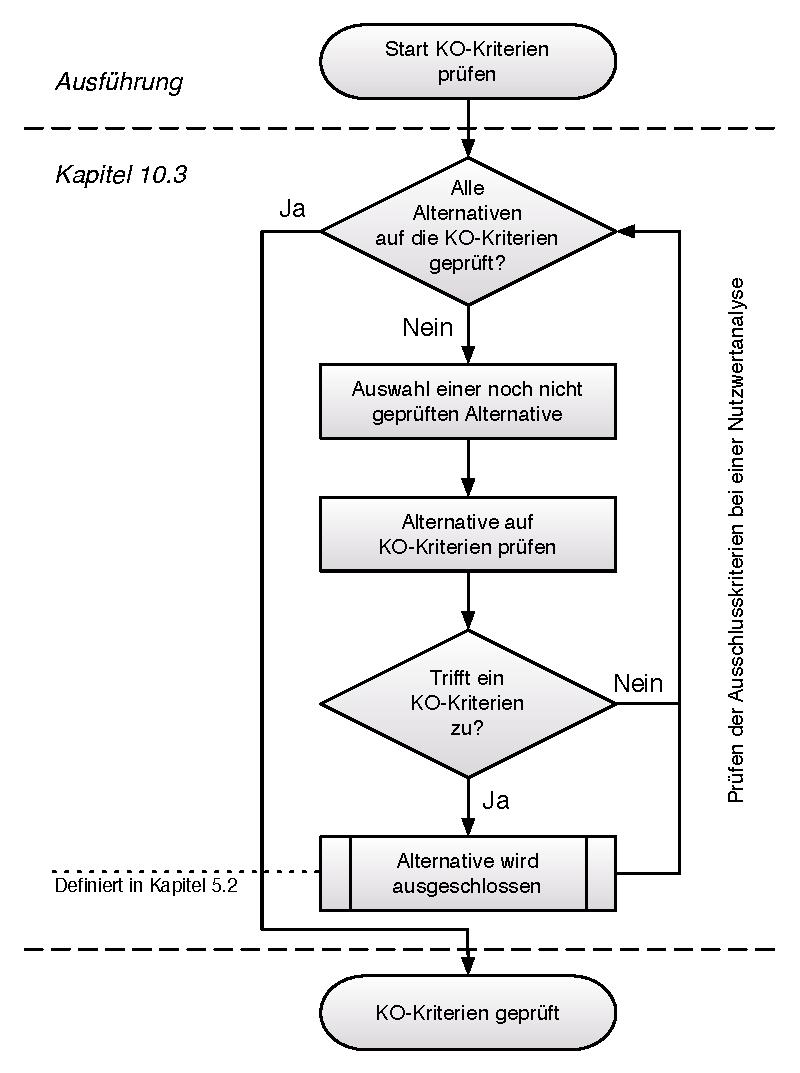
\includegraphics[width=0.7\textwidth]{./image/rahmenbedingungenPruefen.pdf}
      \caption{Die Alternativen sollen gegen KO-Kriterien geprüft werden.}
      \label{img:rahmenbedingungenPruefen}
    \end{center}
  \end{figure}
  
  \clearpage
 
  \section{Analytic Hierarchy Process}
  
  Der Analytic Hierarchy Process stamt aus der Feder eines Mathematikers. Aus
  diesem Grund ist das Verfahren auch einiges Anspruchsvoller als eine
  gewichtete Nutzwertanalyse. Ich gehe hier nicht auf die ganzen Details ein, da
  es den Rahmen der Diplomarbeit übersteigen würde. Totzdem soll eine grober
  Überblick über den \ac{AHP} gegeben werden.
  
  Der \ac{AHP} besteht aus drei Phasen, siehe \cite{AnalyticHierarchyProcess}: 
  
  \begin{enumerate}
    \item Sammeln der Daten
    \item Daten vergleichen und gewichten
    \item Daten verarbeiten
  \end{enumerate}
  
  \subsection{Sammeln der Daten}
  
  In der ersten Phase sollen alle Daten, die für eine Entscheidungsfindung
  erheblich sind, gesammelt werden.
  
  \begin{itemize}
    \item Zuerst soll eine konkrete Frage formuliert werden, für welche die
    beste Antwort gesucht wird.
    \item Danach sollen zu der gestellten Frage alle Kriterien  gesucht werden,
    welche die Lösung beeinflussen können.
    \item Als letztes sollen alle Alternativen gesucht werden, welche als
    mögliche Lösung infrage kommen.
  \end{itemize}
  
  \subsection{Daten vergleichen und gewichten}
  
  In der zweiten Phase folgt nun die Gegenüberstellung, Vergleich und Bewertung
  aller Kriterien beziehungsweise Alternativen in zwei Unterschritten.
  
  \begin{itemize}
    \item Jedes Kriterium wird jedem anderen gegenübergestellt und darauf
    verlgichen, was eine grössere Bedeutung in der gestellten Frage hat. Die
    Skala geht von 1 bis 9, siehe Tabelle \ref{tab:vergleichsgrade}.
    \item Für jedes Kriterium wird jede mögliche Alternativen mit jeder anderen
    gegenübergestellt und auf ihre Eignung hin untersuchen, welche Alternative
    am besten zur Erfüllung des jeweiligen Kriteriums passt. Die Skala geht von
    1 bis 9, siehe Tabelle \ref{tab:vergleichsgrade}.
  \end{itemize}
  
  \begin{table}[ht]
    \sffamily 
    \begin{center}
      \begin{tabular}{lc}
        \toprule
        \textbf{Bedeutung} & \textbf{Skala}\\
        \midrule
        gleiche Bedeutung & 1\\
        leicht grössere Bedeutung & 2 - 3\\
        viel grössere Bedeutung & 4 - 6\\
        erheblich grössere Bedeutung & 7 - 8\\
        absolut dominierend & 9\\
        \bottomrule
      \end{tabular}
      \caption{Skala der Vergleichsgrade}
      \label{tab:vergleichsgrade}
    \end{center}
  \end{table}
    
  \subsection{Daten verarbeiten}
  
  Mit einem mathematischen Modell, kann der \ac{AHP} nun eine präzise Gewichtung
  aller Kriterien errechnen. Mit der Gewichtung der Kriterien und dem Vergleich
  der Alternativen, kann der \ac{AHP} nun berechnen, welches die beste Lösung
  (Alternative) für die gestellt Frage ist. Aus dem mathematischen Modell
  heraus, kann nun ein Inkonsistenzfaktor errechnet werden, der eine Aussage
  macht, wie logisch die Bewertungen zueinander sind.
  
  Diese Berechnungen werden meistens mit der Unterstütztung einer Software
  gemacht. Als Beispiel gibt es JAHP 2.1\footnote{Für Hintergrundinformationen
  zum JAHP 2.1, siehe \cite{JAHP}}, dies ist ein Java Programm mit dem der
  gesammte Prozess des \ac{AHP} abgebildet und berechnet werden kann. Das
  Programm wird unter den Bedingungen der GNU General Public License
  vertrieben.
    
  \section{Kombination beider Methoden}
  
  Diese beiden Methoden können auch kombiniert eingesetzt werden, siehe
  \cite{AhpNwaKombination}, da der \ac{AHP} relativ komplex in der Umsetztung
  ist. Als Kombination kann die Nutzwertanalyse als Methode verwendet werden,
  und der \ac{AHP} wird für die präzise Berechnung der Gewichtung einzelner
  Entscheidungskriterien verwendet. Aus der Kombination entsteht somit eine
  neue Methode, welche durch die Verständlichkeit der \ac{NWA} und der
  objektiven Gewichtung des \ac{AHP} eine plausable Evaluation ermöglicht.

  \subsection{Verbesserung der 
  Gewichtung}\label{subsection:VerbesserungDerGewichtung}
  
  Damit die Gewichtung noch präziser bestimmt werden kann, gibt es verschiedene
  Ansätze. Zwei Ansätze möchte ich hier erläutern:
  
  \begin{itemize}
    \item Die Sensitivitätsanalyse, siehe \cite{Sensitivitaetsanalyse}.
    
    Dabei wird ein einzelner Werte in der Gewichtung gezielt verändert, und das
    Resultat wird danach geprüft. Bei der Methode des \ac{AHP} könnte zum
    Beispiel der Inkonsistenzfaktor geprüft werden, wenn dieser sich Positiv
    verändert, dann zeigt das eine Vergesserung der Gewichtung. Das Vorgehen
    wird iterativ, bis zur Unterschreitung einer definierten Schwelle des
    Inkonsistenzfaktors, fortgeführt.
    
    \item Statistische Methoden, wie der Mittelwert oder der Median, siehe
    \cite{Median} und \cite{Mittelwert}.
    
    Dabei wird der Prozess der Gewichtung von mehr als einer Person
    durchgeführt. Das Ergebniss wird aufgrund der statistischen Methoden
    normalisiert, was zu einem objektiveren Resultat führen wird.
  \end{itemize}
  
  Diese Ansätze zur Verbesserung der Gewichtung werden im Rahmen der
  Diplomarbeit nicht durchgeführt, sollen aber bei einer weiteren Anwendung
  nicht ausgeschlossen werden.
  
  \section{Integration in die IT-Infrastruktur prüfen}
  
  Damit ein Java Web Framework in der IT-Infrastruktur betrieben werden kann,
  muss es deren Ansprüchen genügen. Es soll in einer Analysephase die
  IT-Infrastruktur untersucht werden. Es soll analysiert werden, welche Version
  des \ac{JRE} zur Verfügung gestellt wird, zusätzlich sollen die eingesetzten
  Serverkomponenten veranschaulicht werden. Ein Augenmerk soll auch auf
  eingesetzte Protokolle für die Kommunikation, sowie auf die vorgegebene
  logische und physische Trennung von Schichten in der Serverinfrastruktur
  gelegt werden.
  
  Wenn die Auswahl der zu evaluierenden Java Web Frameworks getroffen wurde,
  soll aufgrund der analysierten IT-Infrastruktur geprüft werden, ob ein Betrieb
  möglich ist. Falls der Betrieb nicht möglich wäre, würde das Java Web
  Framework aus der Evaluation ausgeschlossen werden. Der genaue Ablauf ist als
  Flussdiagramm in der Abbildung \ref{img:integrationPruefen} ersichtlich.
  
  \clearpage
  
  \begin{figure}[h!]
    \begin{center}
      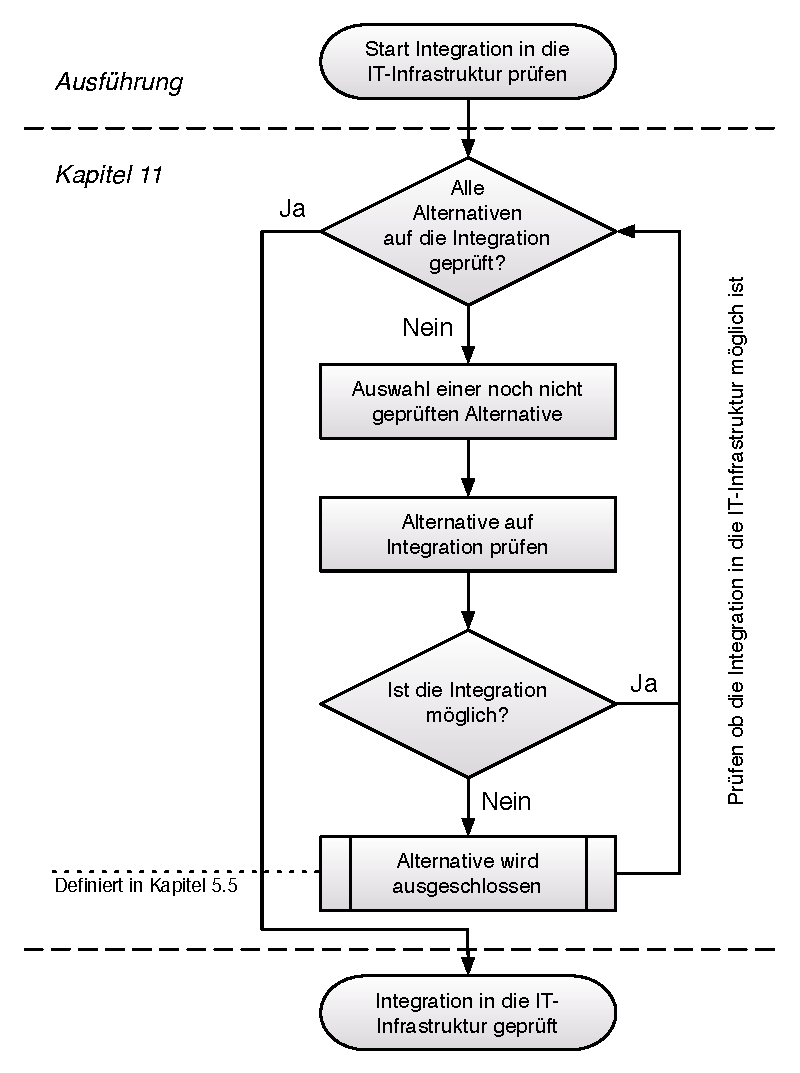
\includegraphics[width=0.7\textwidth]{./image/integrationPruefen.pdf}
      \caption{Es soll geprüft werden, ob die Integration in die
      IT-Infrastruktur möglich ist}
      \label{img:integrationPruefen}
    \end{center}
  \end{figure}
  
  \section{Abdeckung der GUI-Komponenten und Paradigmen}
  
  Da die Evaluation gemacht wird, um bestehende Java Swing Applikationen
  abzulösen, soll auch ein Fokus auf das \ac{GUI} gelegt werden. Im Kapitel
  \ref{chapter:MethodenZurAnalyseVonJavaSwingApplikationen}
  (\nameref{chapter:MethodenZurAnalyseVonJavaSwingApplikationen}, S.
  \pageref{chapter:MethodenZurAnalyseVonJavaSwingApplikationen}ff) wird
  beschrieben, wie besetehende Java Swing Applikationen analysiert werden
  können. Das daraus resultierende Ergebnis soll als Grundlage für die Prüfung
  der Abdeckung der GUI-Komponenten und Paradigmen dienen.
  
  Die Prüfung der Abdeckung zielt darauf ab, herauszufinden, ob eine
  Implementierung mit dem zu evaluierenden Java Web Framework, sinnvoll machbar
  ist. Dabei werden alle erkannten GUI-Komponenten und GUI-Paradigmen der
  analysierten Java Swing Applikationen genommen und mit der Dokumentation des
  zu evaluierenden Java Web Frameworks verglichen. Im diesem Vergleich soll
  festgestellt werden, ob eine Komponente oder ein Pardigma äquivalent
  umsetzbar ist. Der Vergleich findet für jede Komponente und jedes
  Paradigma statt und soll schlussendlich in der Form einer prozentualen
  Abdeckung dokumentiert werden.
  
  Die jeweiligen Prozentangaben berechnen sich wie in den beiden Formeln
  \ref{eq:AbdeckungGuiKomponenten} und \ref{eq:AbdeckungGuiParadigmen}
  dargestellt.

  \begin{equation}
    \label{eq:AbdeckungGuiKomponenten}
    Abdeckung\;GUI\;Komponenten = \frac
    	{gefundene\;GUI\;Komponenten}
    	{mögliche\;GUI\;Komponenten} * 100
  \end{equation}

  \begin{equation}
    \label{eq:AbdeckungGuiParadigmen}
    Abdeckung\;GUI\;Paradigmen = \frac
    	{gefundene\;GUI\;Paradigmen}
    	{mögliche\;GUI\;Paradigmen} * 100
  \end{equation}
  
  Als Voraussetzung, das sich das Java Web Framework für eine mögliche Ablösung
  eignet, soll eine Mindestabdeckung von 80\% aller Komponenten und
  Paradigmen erreicht werden. Diese Schwelle ist verhandelbar und wurde in
  diesem Fall aufgrund des Paretoprinzips\footnote{Das Paretoprinzip, auch
  80-zu-20-Regel, besagt, dass 80\% der Ergebnisse in 20\% der Gesamtzeit eines
  Projekts erreicht werden. Die verbleibenden 20\% der Ergebnisse verursachen
  die meiste Arbeit, siehe \cite{Paretoprinzip}.} gewählt. Der Gedanke dahinter
  ist, dass in einem möglichen Projekt zur Ablösung von einer Java Swing
  Applikation mit dem zu evaluierenden Java Web Framework, in 20\% der Zeit die
  meisten Views äquivalent implementiert werden können. Für die eventuell
  fehlenden GUI-Komponenten oder GUI-Paradigmen sollte dann genügend Zeit zur
  Verfügung stehen, um einen Workaround in der Implementierung auszuarbeiten.
  
  Ob eine Schwelle von 80\% genügend ist, sei dahingestellt, dies sollte in
  einer weiteren Anwendung dieser Methode neu geprüft werden. In der Anwendung
  im Rahmen dieser Diplomarbeit wird ein Java Web Framework, welches eine
  Abdeckung von weniger als 80\% hat, aus der Evaluation ausgeschlossen. Dies
  wird in der Abbildung \ref{img:implementierungPruefen} als Flussdiagramm
  veranschaulicht.
  
  Natürlich wird auf eine möglichst hohe Gesamtabdeckung abgezielt. Wenn zwei
  Java Web Frameworks den selben Nutzwert ausweisen, soll das Framework mit der
  höheren Gesamtabdeckung der GUI-Komponenten und Paradigmen präferiert werden.
  Die Gesamtabdeckung berechnet sich wird wie in der Formel
  \ref{eq:AbdeckungGuiTotal} dargestellt.
  
  \begin{equation}
    \label{eq:AbdeckungGuiTotal}
    Gesamtabdeckung = \frac
    	{gefundene\;Komponenten\;\&\;Paradigmen}
    	{mögliche\;Komponenten\;\&\;Paradigmen} * 100
  \end{equation} 

  \begin{figure}[h!]
    \begin{center}
      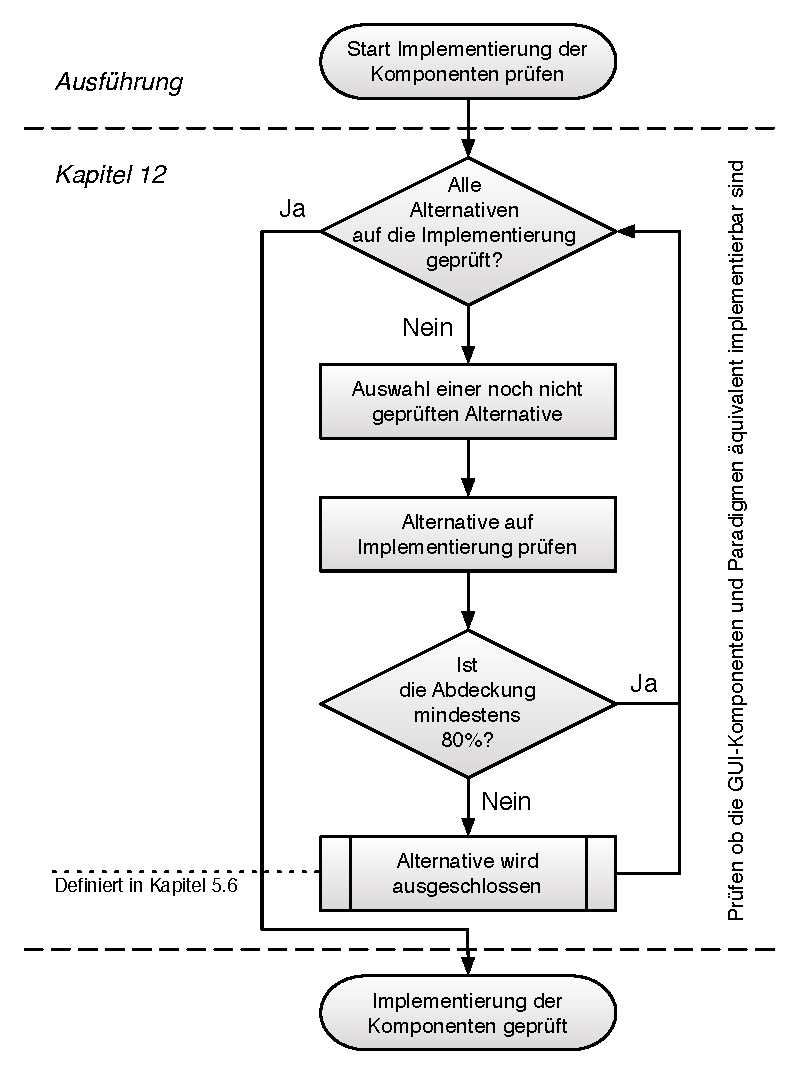
\includegraphics[width=0.7\textwidth]{./image/implementierungPruefen.pdf}
      \caption{Es soll geprüft werden, ob die GUI-Komponenten und Paradigmen
      implementiert werden können}
      \label{img:implementierungPruefen}
    \end{center}
  \end{figure}  
  
  \section{Proof of Concept}
  
  Für diejenige Alternative, für welche der höchste Nutzwert errechnet wurde,
  die in die IT-Infrastruktur der \ac{ZKB} integriert werden kann und die eine
  Mindestabdeckung von 80\% der gefundenen GUI-Komponenten und Paradigmen
  aufweist, soll in einem Proof of Concept anhand eines Prototypen gezeigt
  werden, dass sich die Evaluationsmethode bewährt hat.
  
  Die Definition der Anforderungen an den Prototypen werden mit der Technik der
  User Stories gemacht, siehe \cite{UserStories}.
  
  \subsection{Was sind User Stories}
  
  User Stories beschreiben Anforderungen an eine Software in einer für Jedermann
  verständlichen Sprache. Es sollen keine technischen Details genannt, sondern
  viel eher Eigenschaften erläutert werden, die jeder versteht. Oft werden User
  Stories als Aktionen in einem \ac{GUI} verfasst. Aus den User Stories kann
  man jeweils Akzeptanztests \cite{AcceptanceTests} ableiten.
  
  Eine User Story sollte nicht mehr als drei Sätze haben. Das kommt daher, dass
  eine User Story nie zu komplex sein darf. Wenn man mehr als drei Sätze für die
  Beschreibung einer User Story braucht, sollte diese in mehrere kleinere User
  Stories aufgeteilt werden, welche genug simpel sind, um wiederum in drei
  Sätzen beschrieben zu werden.
  
  Jede User Story wird mit einer eindeutigen Nummer versehen: US-\{User Story
  Nummer\}
  
  \subsection{Priorisierung der User Stories}
  
  Es soll eine Priorisierung der definierten User Stories gemacht werden. Die
  Prioritäten werden in \begin{itshape}hoch\end{itshape},
  \begin{itshape}mittel\end{itshape} und
  \begin{itshape}tief\end{itshape} eingeteilt. Es sollen nur die ``hoch''
  priorisierten User Stories umgesetzt werden.
  
  \subsection{Akzeptanztests zur Prüfung}
  
  Aus den ``hoch'' priorisierten User Stories können nun Akzeptanztests
  abgeleitet werden. Eine User Story ist dann fertig und erfolgreich,
  wenn sie technisch umgesetzt wurde und die dazu definierten Akzeptanztests
  abgenommen wurden. Jeder Akzeptanztest wird mit einer eindeutigen Nummer
  versehen: T-\{User Story Nummer\}.\{Test Nummer\}
  
  Der Proof of Concept ist dann erfolgreich, wenn alle Akzeptanztest erfolgreich
  abgenommen wurden.
  
  Falls die Akzeptanztests nicht erfolgreich abgenommen werden konnten, zeigt
  das, dass mit der Evaluation des Java Web Frameworks eine ungenügende
  Alternative empfohlen wurde.
    
  \section{Ablauf einer Evaluation}
  
  In der Abbildung \ref{img:ablaufEvaluation} ist der komplette Ablauf einer
  Evaluation mit der kombinierten Methode aus Nutzwertanalyse und
  \ac{AHP} ersichtlich.
  
  \begin{figure}[h!]
    \begin{center}
      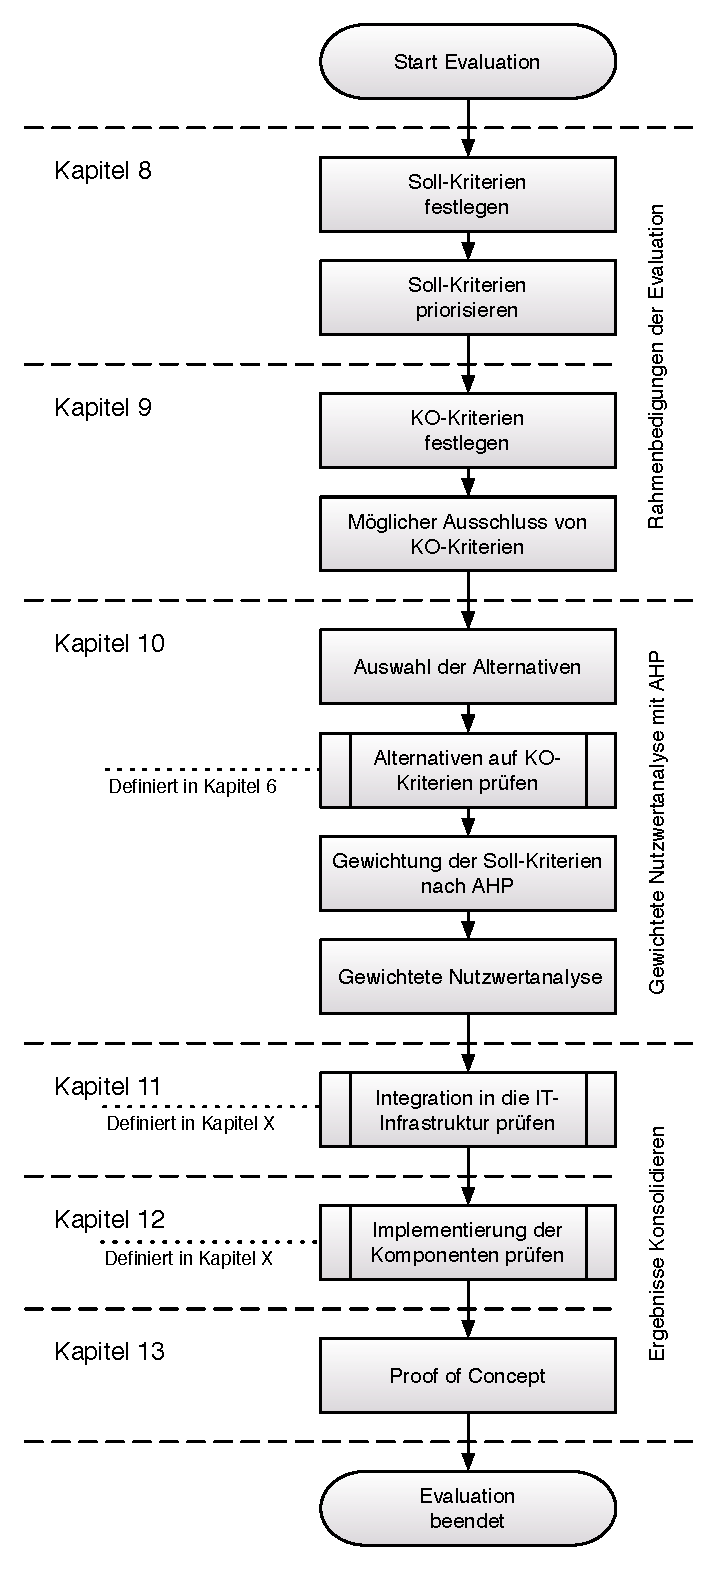
\includegraphics[width=0.7\textwidth]{./image/kompletterAblaufDerEvaluation.pdf}
      \caption{Ablauf einer Evaluation mit der kombinierten Methode aus
      Nutzwertanalyse und \ac{AHP}}
      \label{img:ablaufEvaluation}
    \end{center}
  \end{figure}


  \cleardoublepage
   
  % ===========================================================================
  % Kapitel XXX beginns here
  % ===========================================================================
   
  \chapter{Analyse der Java Swing
  Applikationen}\label{chapter:AnalyseDerJavaSwingApplikationen}
  
    Dieses Kapitel behandelt die Analyse von Java Swing Applikationen. Die
  Analyse betrifft die Swing Komponenten, und Komponenten die in einen
  Zusammenhang mit Swing Komponenten stehen. Es werden die gezeigten
  Methoden zur Analyse von Java Swing Applikationen aus dem Kapitel 
  \ref{chapter:MethodenZurAnalyseVonJavaSwingApplikationen}
  (\nameref{chapter:MethodenZurAnalyseVonJavaSwingApplikationen}, S.
  \pageref{chapter:MethodenZurAnalyseVonJavaSwingApplikationen}ff) angewendet.
  Als Ergebnis wird eine Kategorisierung der verwendeten Swing Komponenten
  aufgelistet. Der Ablauf wird in der Abbildung
  \ref{img:kompletteApplikationsAnalyse} dargestellt.
  \newline

  
  \section{Auswahl der Java Swing Applikationen}
  
  Es sollen drei Applikationen, welche von der Zürcher Kantonalbank entwickelt
  wurden, analysiert werden. Die Applikationen sollen mit Java Swing entwickelt
  worden sein. Die Applikationen werden in der Tabelle
  \ref{tab:zuAnalysierendeJavaSwingApplikationen} aufgelistet.
  \newline
  
  \begin{table}[ht]
    \sffamily 
    \begin{center}
      \begin{tabular}{llp{2cm}p{3.5cm}}
        \toprule
        \textbf{Applikation} & \textbf{Version} & \textbf{Sourcecode vorhanden}
        & \textbf{GUI enthält sensible Informationen}\\
        \midrule
        Strukti Live & 1.2 & Ja & Nein\\
        Strukti Online & 2.10.0 & Ja & Ja\\
        Hedo Tool & 1.0.710 & Ja & Ja\\
        \bottomrule
      \end{tabular}
      \caption{Zu analysierende Java Swing Applikationen}
      \label{tab:zuAnalysierendeJavaSwingApplikationen}
    \end{center}
  \end{table}
  
  \section{Begründung}
  
  \begin{description}
  \item[Strukti Live]
  Wurde gewählt, weil diese Applikation von der ZKB veröffentlicht wurde. Somit
  werden bei der Analayse keine sensiblen Informationen preisgegeben.
  
  \item[Strukti Online]
  Wurde gewählt, weil eine mögliche Migration zur Web Applikation schon einmal
  in der \ac{ZKB} zur Diskussion stand.
  
  \item[Hedo Tool]
  Wurde gewählt, da die Applikation über ein hochstehendes \ac{GUI} verfügt.
  \end{description}
  
  \section{Strukti Live}
  
  Strukti Live ist ein Lerntool der Zürcher Kantonalbank für strukturierte
  Produkte. Die Applikation kann auf dem Internetauftritt \footnote{Unter 
  \url{http://www.zkb.ch/struktilive} sind alle nötigen Informationen zu Strukti
  Live enthalten.} der \ac{ZKB} heruntergeladen werden. Es wurde die aktuelle
  Version 1.2 für die Analyse verwendet.
  
  In der Tabelle \ref{tab:bibliothekenStruktiLive} sind alle verwendeten
  Bibliotheken, welche eine Interaktion mit dem \ac{GUI} haben, ersichtlich.
  \newline
  
  \begin{table}[ht]
    \sffamily 
    \begin{center}
      \begin{tabular}{lp{4.5cm}ccp{2cm}}
        \toprule
        \textbf{Bibliothek} & \textbf{Funktion} & \textbf{Version} &
        \textbf{Lizenz} & \textbf{Quellcode vorhanden}\\
        \midrule
        core-renderer.jar & XHtml und CSS Renderer für Swing & R8 & LGPL & Ja\\
        %bogatyr\_0.60.jar & Abstraktion einiger Swing Komponenten & 0.60 & GPL
        %& Ja\\
        jfreechart-1.0.10.jar & Charting Library für Java & 1.0.10 & LGPL & Ja\\
        %jcommon-1.0.13.jar & JFreeChart extension & 1.0.13 & LGPL & Ja\\
        %ZKB\_CICD\_0.40.jar & Swing Komponenten im ZKB Design & 0.40 & - & Ja\\
        \bottomrule
      \end{tabular}
      \caption{Verwendete Bibliotheken von Strukti Live 1.2}
      \label{tab:bibliothekenStruktiLive}
    \end{center}
  \end{table}
  
  \subsection{Gefundene Komponenten}
  
  \subsubsection{Top-Level-Komponenten}
  
  \begin{itemize}
    \item \(javax.swing.JDialog\), siehe Abbildung \ref{img:SL-02}
    \item \(javax.swing.JFrame\), siehe Abbildung \ref{img:SL-01}
  \end{itemize}
  
  \subsubsection{Intermediate-Komponenten}
  
  \begin{itemize}
    \item \(javax.swing.JPanel\), siehe Abbildung \ref{img:SL-01}
    \item \(javax.swing.JRootPane\), siehe Abbildung \ref{img:SL-01}
    \item \(javax.swing.JScrollPane\), siehe Abbildung \ref{img:SL-01}
    \item \(javax.swing.JTabbedPane\), siehe Abbildung \ref{img:SL-03}
  \end{itemize}
  
  \subsubsection{Atomic-Komponenten}
  
  \begin{itemize}
    \item \(javax.swing.JButton\), siehe Abbildung \ref{img:SL-01}
    \item \(javax.swing.JCheckBox\), siehe Abbildung \ref{img:SL-01}
    \item \(javax.swing.JLabel\), siehe Abbildung \ref{img:SL-01}
    \item \(javax.swing.JRadioButton\), siehe Abbildung \ref{img:SL-02}
    \item \(javax.swing.JSlider\), siehe Abbildung \ref{img:SL-02}
    \item \(javax.swing.JTextField\), siehe Abbildung \ref{img:SL-02}
    \item \(javax.swing.JToolTip\), siehe Abbildung \ref{img:SL-03}
  \end{itemize}
  
  \subsubsection{Spezielle Komponenten}
  
  \begin{itemize}
    \item \(javax.swing.JLabel\) als externer Link, siehe Abbildung
    \ref{img:SL-03}
    \item \(org.jfree.chart.JFreeChart\), siehe Abbildung \ref{img:SL-02}
    \item \(org.xhtmlrenderer.simple.XHTMLPanel\), siehe Abbildung
    \ref{img:SL-03}
  \end{itemize}
  
  \begin{figure}[htb]
    \begin{center}
      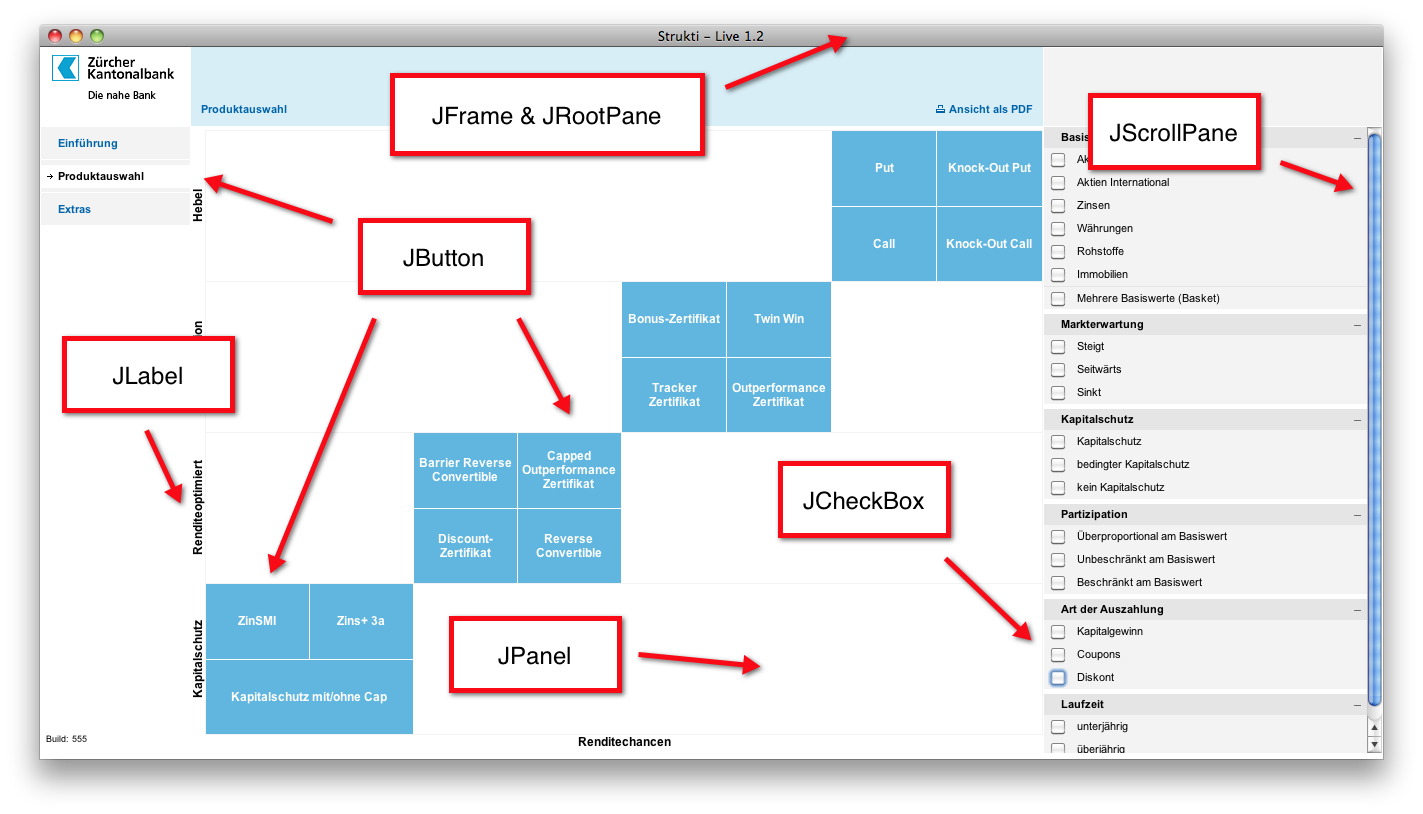
\includegraphics[width=\textwidth]{./image/SL/SL-01.png}
      \caption{Strukti Live 1.2 - Screenshot I}
      \label{img:SL-01}
    \end{center}
  \end{figure}
  
  \begin{figure}[htb]
    \begin{center}
      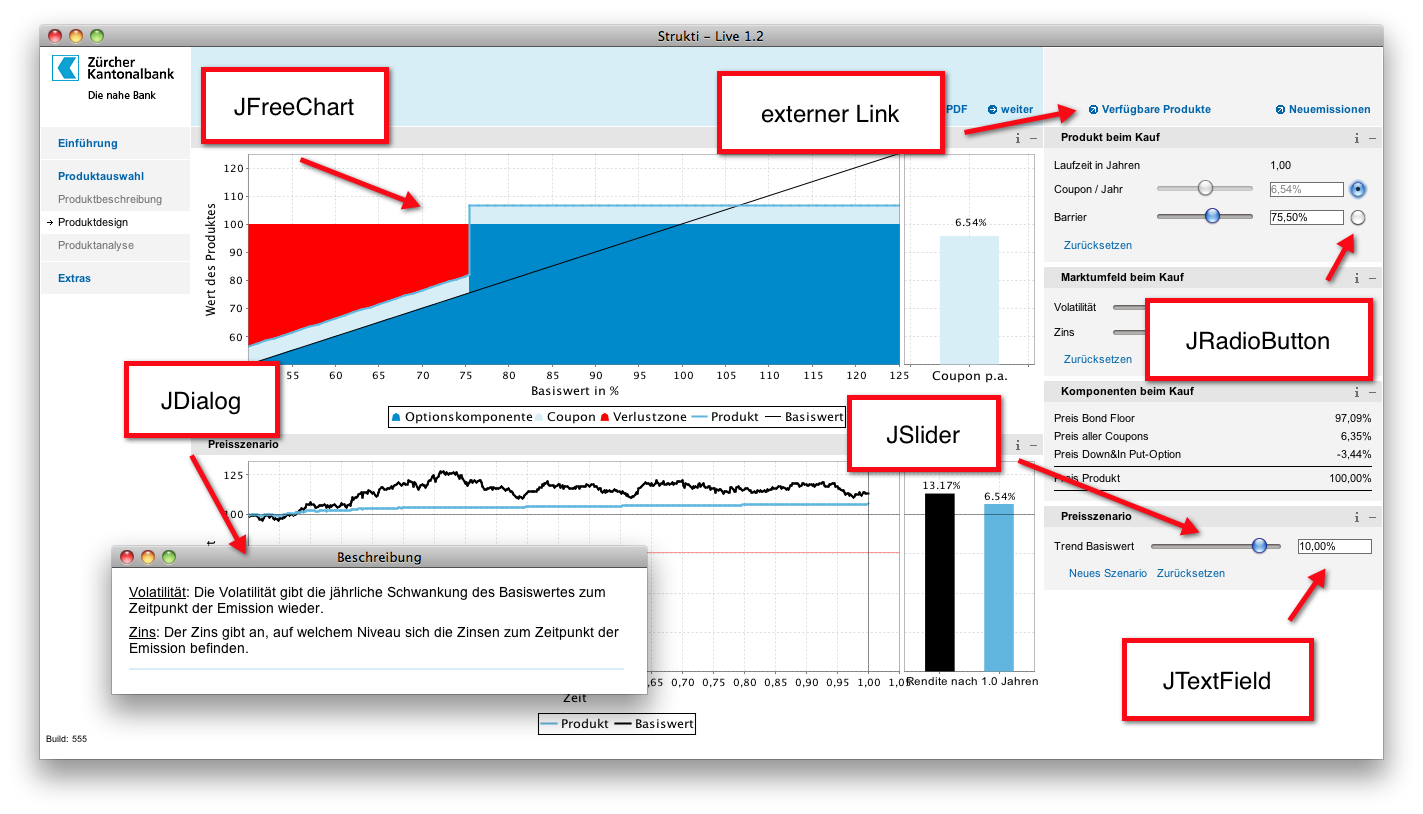
\includegraphics[width=\textwidth]{./image/SL/SL-02.png}
      \caption{Strukti Live 1.2 - Screenshot II}
      \label{img:SL-02}
    \end{center}
  \end{figure}
  
  \begin{figure}[htb]
    \begin{center}
      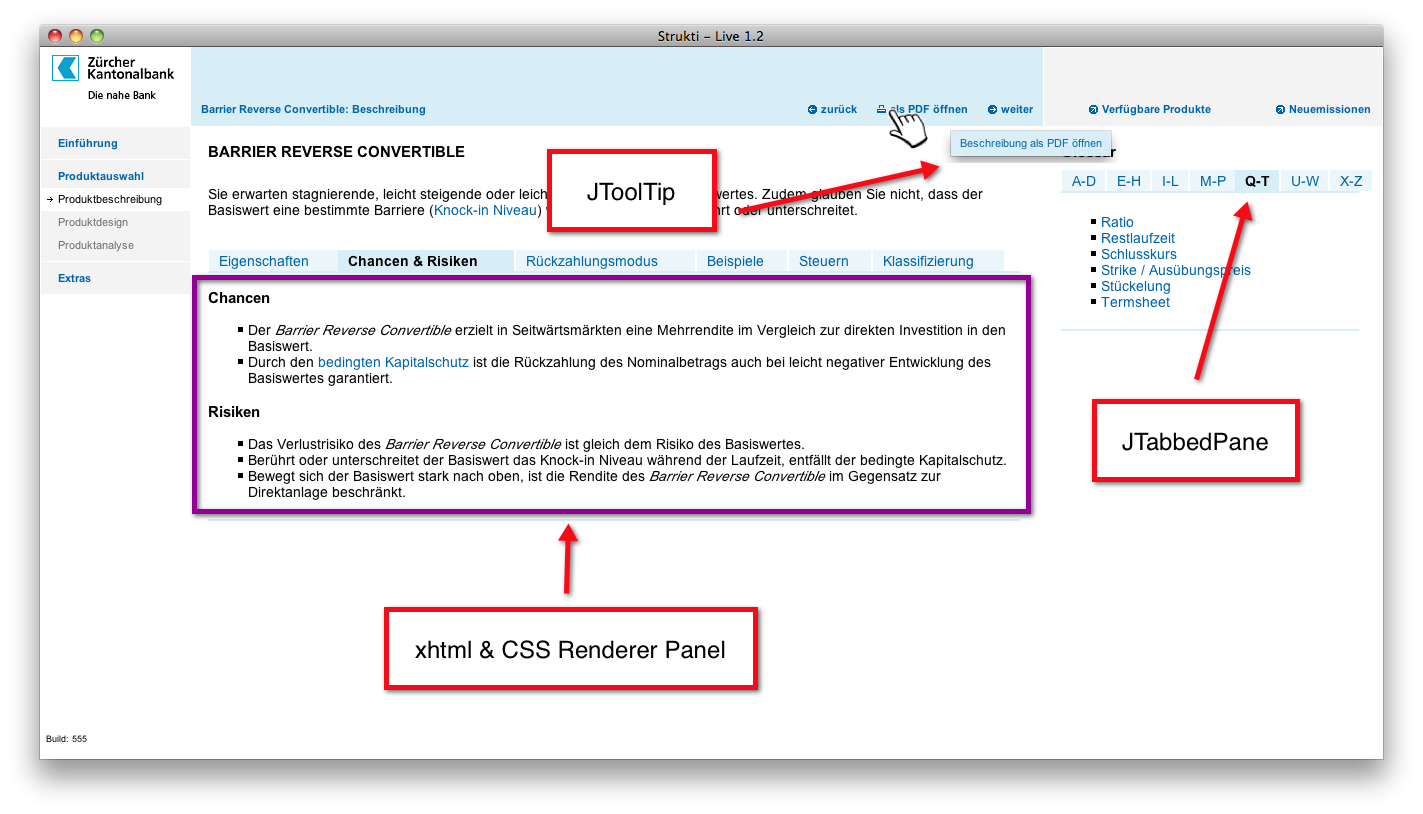
\includegraphics[width=\textwidth]{./image/SL/SL-03.png}
      \caption{Strukti Live 1.2 - Screenshot III}
      \label{img:SL-03}
    \end{center}
  \end{figure}
  
  \subsection{Gefundene Design-Patterns}
  
  \begin{description}
    \item[Observer]
    Die Menüführung wurde durch das Observer-Pattern\footnote{Siehe
    \cite{GUIDesignPatterns} S. 2ff} implementiert. Dabei wird in einem
    Modell durch das Drücken eines \(javax.swing.JButton\) der jeweilige Status
    der Applikation angepasst. Die entsprechen \(javax.swing.JPanel\), welche
    auf Änderungen des Modells hören, können sich dann jeweils neu
    zeichnen.

    Ebenfalls mit dem Observer-Pattern realisiert wurde die Aktualisierung
    von Komponenten welche zusammen hängen. Als Beispiel dient ein Verbund der
    Komponenten \(javax.swing.JTextField\), \(javax.swing.JSlider\) und für die
    grafische Darstellung \(org.jfree.chart.JFreeChart\). Dabei werden bei
    einer Änderung des Wert bei dem \(JSlider\) oder dem \(JTextfeld\) die Werte
    aller anderen Komponenten entsprechend aktualisiert.
  \end{description}
  
  \subsection{Gefundene ``neue'' Komponenten}
  
  \begin{description}
    \item[Button-Matrix]
    \(JButtons\) werden in einer Matrix angeordnet, um sie entsprechend ihrer
    Funktion zu ordnen. Hinter jedem \(JButton\) steckt ein Finanzprodukt, das
    bei einem Klick angezeigt werden kann. Die \(JButtons\) können entsprechend
    ihrer Renditechancen (x-Achse) und deren Kapitalschutzes (y-Achse)
    angeordnet werden.
    \item[Akkordeon]
    Ein Verbund von \(javax.swing.JPanel\) Komponenten, bei welchem ein
    \(JPanel\) als Titelleiste funktioniert. In der Titelleiste kann über ein
    Minus- oder Plussymbol ein weiterer \(JPanel\) ein- oder ausgeklappt werden.
    Zudem gibt es in der Titelleiste ein \(JButton\), wo ein Dialog mit
    Hintergrundinformationen geöffnet werden kann.
  \end{description}
  
  \section{Strukti Online}
  
  Strukti Online ist ein Emissionstool der \ac{ZKB} für strukturierte Produkte.
  Die Applikation wird aktuell nur für den internen Gebrauch entwickelt und
  basiert auf Java Swing. Es wurde die aktuelle Version 2.10.0 für die Analyse
  verwendet.
  
  Da es sich um eine interne Applikation handelt, werden keine Screenshots
  der Applikation gezeigt, da anhand dessen eventuell Rückschlüsse auf die
  Business-Logik gemacht werden könnte.
  
  In der Tabelle \ref{tab:bibliothekenStruktiOnline} sind alle verwendeten
  Bibliotheken, welche eine Interaktion mit dem \ac{GUI} haben, ersichtlich,
  und ob deren Sourcecode zugänglich ist.
  
  \begin{table}[ht]
    \sffamily 
    \begin{center}
      \begin{threeparttable}
        \begin{tabular}{lp{4.5cm}ccp{2cm}}
          \toprule
          \textbf{Bibliothek} & \textbf{Funktion} & \textbf{Version} &
          \textbf{Lizenz} & \textbf{Quellcode vorhanden}\\
          \midrule
          core-renderer.jar & XHtml und CSS Renderer für Swing & R8 & LGPL &
          Ja\\
          jfreechart-1.0.10.jar & Charting Library für Java & 1.0.10 & LGPL
          & Ja\\
          forms.jar & Layout System aus der JGoodies Palette & 1.2.1 &
          BSD\tnote{1} & Ja\\
          swingx-1.0.jar & Swing Komponenten Erweiterung & 1.0 & LGPL & Ja\\
          \bottomrule
        \end{tabular}
        \caption{Verwendete Bibliotheken von Strukti Online 2.10.0}
        \label{tab:bibliothekenStruktiOnline}
        \begin{tablenotes}[++]\footnotesize 
          \item[1] Es handelt sich dabei um die ``BSD open source license''
        \end{tablenotes} 
      \end{threeparttable}
    \end{center}
  \end{table}
  
  \subsection{Gefundene Komponenten}
  
  \subsubsection{Top-Level-Komponenten}
  
  \begin{itemize}
    \item \(javax.swing.JDialog\)
    \item \(javax.swing.JFrame\)
  \end{itemize}
  
  \subsubsection{Intermediate-Komponenten}
  
  \begin{itemize}
    \item \(javax.swing.JLayerdPane\)
    \item \(javax.swing.JPanel\)
    \item \(javax.swing.JRootPane\)
    \item \(javax.swing.JScrollPane\)
    \item \(javax.swing.JTabbedPane\)
  \end{itemize}
  
  \subsubsection{Atomic-Komponenten}
  \begin{itemize}
    \item \(javax.swing.JButton\)
    \item \(javax.swing.JCheckbox\)
    \item \(javax.swing.JComboBox\)
    \item \(javax.swing.JFileChooser\)
    \item \(javax.swing.JLabel\)
    \item \(javax.swing.JRadioButton\)
    \item \(javax.swing.JPasswordField\)
    \item \(javax.swing.JSeparator\)
    \item \(javax.swing.JSlider\)
    \item \(javax.swing.JSpinner\)
    \item \(javax.swing.JTable\)
    \item \(javax.swing.JTextArea\)
    \item \(javax.swing.JTextField\)
    \item \(javax.swing.JTextPane\)
    \item \(javax.swing.JToolTip\)
  \end{itemize}
  
  \subsubsection{Spezielle Komponenten}
    
  \begin{itemize}
    \item \(javax.swing.JLabel\) als externer Link
    \item \(org.jfree.chart.JFreeChart\)
    \item \(org.xhtmlrenderer.simple.XHTMLPanel\)
    \item \(org.jdesktop.swingx.JXBusyLabel\)
    \item \(org.jdesktop.swingx.JXDatePicker\)
  \end{itemize}
    
  \subsection{Gefundene Design-Patterns}
  
  \begin{description}
    \item[MVC]
    Das Zusammenspiel von Model, View und Kontroller wurde strikte nach dem
    MVC Design-Pattern\footnote{Siehe \cite{GUIDesignPatterns} S. 15ff.}
    implementiert.
    
    \item[Observer]
    Einfache Aktualisierungen zwischen Komponenten wurden strikte nach dem
    Observer Design-Pattern\footnote{Siehe \cite{GUIDesignPatterns} S. 2ff.}
    implementiert.
    
    \item[Tabellen-Filter]
    Durch die Verwendung von \(JRadioButton\), \(JComboBox\), \(JXDatePicker\)
    und \(JSpinner\) wurden, bei den meisten Ansicht von Tabellen, Filter gebaut,
    damit die Daten auf das Wesentliche reduziert werden können. Datei wurde
    für jede relevante Spalten der Tabelle, entsprechend deren Datentyp, eine
    dieser Komponenten gewählt.
  \end{description}
  
  \subsection{Gefundene ``neue'' Komponenten}
  
  \begin{description}
    \item[Button-Matrix]
    \(JButtons\) werden in einer Matrix angeordnet, um sie entsprechend ihrer
    Funktion zu ordnen. Hinter jedem \(JButton\) steckt ein spezifisches
    vorbewertetes Finanzprodukt, das bei einem Mouseklick angezeigt werden
    kann. Die \(JButtons\) können entsprechend ihrer Laufzeit (x-Achse) und der
    Underlyings\footnote{Auch Basiswerte genannt, siehe \cite{Basiswerte}} des
    hinterlegten Finanzprodukts (y-Achse) angeordnet werden. Die Matrix, kann
    wie eine Tabelle nach Laufzeiten sortiert werden.
    
    \item[Akkordeon]
    Ein Verbund von \(javax.swing.JPanel\) Komponenten, bei welchem ein
    \(JPanel\) als Titelleiste funktioniert. In der Titelleiste kann über ein
    Minus- oder Plussymbol ein weiterer \(JPanel\) ein- oder ausgeklappt werden.
    
    \item[Zeit-Panel]
    Durch die Kombination einer \(org.jdesktop.swingx.JXDatePicker\) und einer
    \(javax.swing.JSpinner\) Komponente kann ein Datum mit Uhrzeit ausgewählt
    werden.
  \end{description}
  
  \section{Hedo Tool}
  
  Hedo Tool ist eine Applikation zur Gewichtung verschiedener Rating-Modelle
  für Wohneigentum. Die Applikation wird aktuell nur zum internen Gebrauch
  entwickelt und basiert auf Java Swing. Es wird die aktuelle Version 1.0.710
  für die Analyse verwendet.
  
  Da es sich um eine interne Applikation handelt, werden keine Screenshots der
  Applikation gezeigt, da anhand dessen eventuell Rückschlüsse auf die
  Business-Logik gemacht werden könnte.
  
  In der Tabelle \ref{tab:bibliothekenHedoTool} sind alle verwendeten
  Bibliotheken, welche eine Interaktion mit dem \ac{GUI} haben, ersichtlich,
  und ob deren Sourcecode zugänglich ist.
  \newline
  
  \begin{table}[ht]
    \sffamily 
    \begin{center}
      \begin{threeparttable}
        \begin{tabular}{lp{4.5cm}ccp{2cm}}
          \toprule
          \textbf{Bibliothek} & \textbf{Funktion} & \textbf{Version} &
          \textbf{Lizenz} & \textbf{Quellcode vorhanden}\\
          \midrule
          binding-2.0.6.jar & Swing Data Binding Framework aus der JGoodies
          Palette & 2.0.6 & BSD\tnote{1} & Ja\\
          forms.jar & Layout System aus der JGoodies Palette & 1.2.1 &
          BSD\tnote{1} & Ja\\
          swingx-1.0.jar & Swing Komponenten Erweiterung & 1.0 & LGPL & Ja\\
          validation-2.0.1.jar & Validiert und präsentiert Validationsresultate
          & 2.0.1 & BSD\tnote{1} & Ja\\
          \bottomrule
        \end{tabular}
        \caption{Verwendete Bibliotheken von Hedo Tool 1.0.710}
        \label{tab:bibliothekenHedoTool}
        \begin{tablenotes}[++]\footnotesize 
          \item[1] Es handelt sich dabei um die ``BSD open source license''
        \end{tablenotes} 
      \end{threeparttable}
    \end{center}
  \end{table}
  
  \subsection{Gefundene Komponenten}
  
  \subsubsection{Top-Level-Komponenten}
  
  \begin{itemize}
    \item \(javax.swing.JDialog\)
    \item \(javax.swing.JFrame\)
  \end{itemize}
  
  \subsubsection{Intermediate-Komponenten}
  
  \begin{itemize}
    \item \(javax.swing.JLayerdPane\)
    \item \(javax.swing.JPanel\)
    \item \(javax.swing.JRootPane\)
    \item \(javax.swing.JScrollPane\)
  \end{itemize}
  
  \subsubsection{Atomic-Komponenten}
  
  \begin{itemize}
    \item \(javax.swing.JButton\)
    \item \(javax.swing.JCheckbox\)
    \item \(javax.swing.JComboBox\)
    \item \(javax.swing.JFileChooser\)
    \item \(javax.swing.JFormattedTextField\)
    \item \(javax.swing.JLabel\)
    \item \(javax.swing.JMenuBar\)
    \item \(javax.swing.JMenu\)
    \item \(javax.swing.JMenuItem\)
    \item \(javax.swing.JProgressBar\)
    \item \(javax.swing.JSeparator\)
    \item \(javax.swing.JSpinner\)
    \item \(javax.swing.JTable\)
    \item \(javax.swing.JTextField\)
    \item \(javax.swing.JTextPane\)
    \item \(javax.swing.JToolTip\)
  \end{itemize}
  
  \subsubsection{Spezielle Komponenten}
    
  \begin{itemize}
    \item \(javax.swing.JLabel\) als externer Link
    \item \(org.jdesktop.swingx.JXBusyLabel\)
  \end{itemize}
  
  \subsection{Gefundene Design-Patterns} 
  
  \begin{description}
    \item[MVC]
    Das Zusammenspiel von Model, View und Kontroller wurde strikte nach dem
    MVC Design-Pattern\footnote{Siehe \cite{GUIDesignPatterns} S. 15ff.}
    implementiert.
    
    \item[Observer]
    Einfache Aktualisierungen zwischen Komponenten wurden strikte nach dem
    Observer Design-Pattern\footnote{Siehe \cite{GUIDesignPatterns} S. 2ff.}
    implementiert.
    
    \item[Worker]
    Asynchrone Jobs, die viel Rechenzeit in Anspruch nehmen, wurden mit\\
    \(javax.swing.SwingWorker\) gelöst.
  \end{description}
  
  \subsection{Gefundene ``neue'' Komponenten}
  
  Es wurden keine ``neuen'' Komponenten identifiziert.
  
  \section{Liste der Komponenten}
  
  Die Auflistung aller gefunden Komponenten soll die vereinigte Menge aller
  gefundenen Komponenten widerspiegeln. Die Auflistung soll als Grundlage für
  die Analyse, ob eine Implementierung der erkannten Swingkomponenten möglich
  ist, dienen. Folgende 32 Komponenten wurden in den Applikationen gefunden:
  
  \subsection{Top-Level-Komponenten}
  
  \begin{itemize}
    \item \(javax.swing.JDialog\)
    \item \(javax.swing.JFrame\)
  \end{itemize}
  
  \subsection{Intermediate-Komponenten}
  
  \begin{itemize}
    \item \(javax.swing.JLayerdPane\)
    \item \(javax.swing.JPanel\)
    \item \(javax.swing.JRootPane\)
    \item \(javax.swing.JScrollPane\)
    \item \(javax.swing.JTabbedPane\)
  \end{itemize}
  
  \subsection{Atomic-Komponenten}
  
  \begin{itemize}
    \item \(javax.swing.JButton\)
    \item \(javax.swing.JCheckbox\)
    \item \(javax.swing.JComboBox\)
    \item \(javax.swing.JFileChooser\)
    \item \(javax.swing.JFormattedTextField\)
    \item \(javax.swing.JLabel\)
    \item \(javax.swing.JMenuBar\)
    \item \(javax.swing.JMenu\)
    \item \(javax.swing.JMenuItem\)
    \item \(javax.swing.JPasswordField\)
    \item \(javax.swing.JProgressBar\)
    \item \(javax.swing.JRadioButton\)
    \item \(javax.swing.JSeparator\)
    \item \(javax.swing.JSlider\)
    \item \(javax.swing.JSpinner\)
    \item \(javax.swing.JTable\)
    \item \(javax.swing.JTextArea\)
    \item \(javax.swing.JTextField\)
    \item \(javax.swing.JTextPane\)
    \item \(javax.swing.JToolTip\)
  \end{itemize}
  
  \subsection{Spezielle Komponenten}
  
  \begin{itemize}
    \item \(javax.swing.JLabel\) als externer Link
    \item \(org.jfree.chart.JFreeChart\)
    \item \(org.xhtmlrenderer.simple.XHTMLPanel\)
    \item \(org.jdesktop.swingx.JXBusyLabel\)
    \item \(org.jdesktop.swingx.JXDatePicker\)
  \end{itemize}
  
  \section{Liste der GUI Paradigmen}
  
  Die Auflistung aller gefundenen GUI Paradigmen soll die vereinigte Menge aller
  gefundenen GUI Paradigmen widerspiegeln. Die Auflistung soll als Grundlage für
  die Analyse, ob eine Implementierung der erkannten GUI Paradigmen möglich
  ist, dienen. Folgende sieben GUI Paradigmen wurden in den Applikationen
  gefunden:
      
  \subsection{Design-Patterns}
  
  \begin{itemize}
    \item MVC
    \item Observer
    \item Tabellen-Filter
    \item Worker
  \end{itemize}
  
  \subsection{``Neue'' Komponenten}
  
  \begin{itemize}
    \item Button-Matrix
    \item Akkordeon
    \item Zeit-Panel
  \end{itemize}

  \cleardoublepage
  
  % ===========================================================================
  % Kapitel XXX beginns here
  % ===========================================================================
  
  \chapter{Evaluation der Java Web
  Frameworks}\label{chapter:EvaluationDerJavaWebFrameworks}
  
    Dieses Kapitel behandelt die Evaluation der Java Web Frameworks. Es wird die
  kombinierte Methode aus dem Kapitel 
  \ref{chapter:MethodenZurEntscheidungsfindungBeiEinerEvaluation}
  (\nameref{chapter:MethodenZurEntscheidungsfindungBeiEinerEvaluation}, S.
  \pageref{chapter:MethodenZurEntscheidungsfindungBeiEinerEvaluation}ff)
  angewendet. Mit der definition von sinnvollen Rahmenbedingungen soll die
  Evaluation durchgeführt und das Resultate in Form einer Rangliste vorgelegt
  werden.
    
  \section{Rahmenbedingungen für die Evaluierung}
  
  Die Rahmenbedingungen für die Evaluierung werden über Soll-Kriterien und
  KO-Kriterien festgelegt.

  \subsection{Soll-Kriterien}
  
  Die Eignung, der zu evaluierenden Java Web Frameworks, wird durch eine Menge
  von Soll-Kriterien bestimmt. Die Soll-Kriterien bestimmen die Anforderungen,
  welche erfüllt werden sollen. Die Anforderungen stammen von einer
  Projektgruppe der Hochschule für Technik und Wirtschaft Berlin. Die
  Soll-Kriterien werden für den Einsatz in der \ac{ZKB} priorisiert.
  
  Soll-Kriterien sind Vorgaben, die möglichst weitgehend Erfüllt werden sollen.
  Wenn ein solches Kriterium nicht erfüllt werden kann, schliesst das die
  Alternative nicht aus. Jedem Soll-Kriterium wird für die Identifikation eine
  eindeutige ID vergeben. Die ID setzt sich folgendermassen zusammen: 
  \{Soll\}-\{Laufnummer\}.
  
  \subsubsection{Anforderungen an Web Frameworks nach AgileLearn}
  
  Eine Projektgruppe namens AgileLearn von der Hochschule für Technik und
  Wirtschaft Berlin befasst sich mit dem Thema Web Frameworks. Die
  Projektgruppe hat sich die Frage gestellt: ``\begin{itshape}Welche
  Anforderungen müssen bei der Wahl eines Webframeworks berücksichtigt
  werden?\end{itshape}''\footnote{Zitat von Raoul Jaeckel, siehe
  \cite{AnforderungenAnWebframeworks}}. Aus der Fragestellung heraus, haben sie
  18 Anforderungen an ein Web Framework ausgearbeitet, welche öffentlich in
  einem Google-Doc\footnote{Ein Service von Google um Dokumente öffentlich zu
  bearbeiten.} ersichtlich sind.
  
  Folgende Anforderungen stammen aus dem Dokument ``\begin{itshape}18
  Anforderungen an Webframeworks -
  OpenDoc\end{itshape}'', siehe \cite{AnforderungenAnWebframeworks}, und werden
  im Anhang \ref{chapter:18AnforderungenNachAgileLearn}
  (\nameref{chapter:18AnforderungenNachAgileLearn}, S.
  \pageref{chapter:18AnforderungenNachAgileLearn}ff) zusammengefasst und mit
  einer ID versehen.

  \subsection{KO-Kriterien}
  
  Anhand einer Menge von KO-Kriterien wird die Auswahl der Alternativen
  eingeschränkt. Die KO-Kriterien sind aus dem \begin{itshape}Handbuch der
  IT-Architektur\end{itshape}, siehe \cite{ZkbHandbuchDerItArchitektur}, der
  \ac{ZKB} entnommen. Die Namensgebung in dem Handbuch unterscheidet sich
  leicht, es wird nicht von KO-Kriterien, sondern von Grundsätzen gesprochen.
  
  KO-Kriterien sind Vorgaben, welche zwingend erfüllt sein müssen. Falls ein
  Kriterium nicht erfüllt werden kann, fällt die Entscheidung auf diese
  Alternative negativ aus. Jedem KO-Kriterium wird für die Identifikation eine
  eindeutige ID vergeben. Die ID setzt sich folgendermassen zusammen: 
  \{KO\}-\{Laufnummer\}.

  \subsubsection{Grundsätze aus der IT-Architektur der Zürcher Kantonalbank}
  
  Ein Grundsatz wird im Handbuch wer IT-Architektur wie folgt definiert:
  \newline
  
  ``\begin{itshape}Es sind Grundsätze definiert, nach denen sich die Baupläne
  der IT-Systeme zu richten haben. Die Grundsätze sind ein Regelwerk mit
  Weisungscharakter.\end{itshape}''
  \footnote{\cite{ZkbHandbuchDerItArchitektur} Kapitel 1.3 - \begin{itshape}Was
  ist die IT-Architektur der ZKB\end{itshape}, Seite 11}
  \newline

  \noindent
  Dabei gibt es eine Hintertür:
  \newline

  ``\begin{itshape}Grundsätze sind verbindliche Vorgaben (Konventionen), von
  denen nur in begründeten Ausnahmen abgewichen werden kann.\end{itshape}''
  \footnote{\cite{ZkbHandbuchDerItArchitektur} Kapitel 1.8 -
  \begin{itshape}Leseanleitung\end{itshape}, Seite 14}
  \newline
  
  \noindent
  Das Dokument wurde analysiert und alle Grundsätze, welche für diese
  Diplomarbeit relevanten sind, werden im Anhang
  \ref{chapter:GrundsaetzeDerZkbItArchitektur}
  (\nameref{chapter:GrundsaetzeDerZkbItArchitektur}, S.
  \pageref{chapter:GrundsaetzeDerZkbItArchitektur}ff) aufgelistet und mit einer
  ID versehen.

  \section{Priorisierung der Soll-Kriterien}
  
  Da 18 Soll-Kriterien definiert wurden und diese in jeder Alternative 
  untersucht werden müssten, würde das den Rahmen der Diplomarbeit sprengen.
  Desshalb sollen die Soll-Kriterien in eine Hirarchie entsprechend ihrer
  Wichtigkeit für die \ac{ZKB} aufgeteilt werden. Die Hirarchie wird in drei
  Gruppen aufgeteilt:
  
  \begin{itemize}
    \item Wichtig
    \item Nice to have
    \item Unwichtig
  \end{itemize}
  
  Es sollen nur die ``wichtigen'' Soll-Kriterien in die Evaluation mit
  einbezogen werden.
  
  \subsection{Wichtige Aspekte im Software-Lebenszyklus für die ZKB}
  
  \begin{description}
    \item[Sicherheit]
    Nur eine Bank, die als sicher gilt, hat das Vertrauen der Kunden und somit
    Erfolg in ihrem Geschäft.
    \item[Kosten]
    Die laufenden Kosten sollen so tief wie möglich gehalten werden. Gemäss
    Abbildung \ref{img:softwareLifecycleCost} liegen die Hauptkosten im
    Software-Lebenszyklus bei der Maintenance-Phase. Somit können die Kosten für
    requirements Engineering, Design, Programming und Integration vernachlässigt
    werden.
    \item[Ressourcen]
    Damit Software entwickelt und gewartet werden kann, wird die Verfügbarkeit
    von qualifizierten Ressourcen benötigt.
    \item[Image]
    Um sich von der Konkurenz abzuheben wird ein Image aufgebaut das sich
    zeitgemäss, flexibel und inovativ präsentieren soll, siehe
    \cite{WillkommenBeiDerZkb} S. 34ff.
  \end{description}
  
  \begin{figure}[ht]
    \begin{center}
      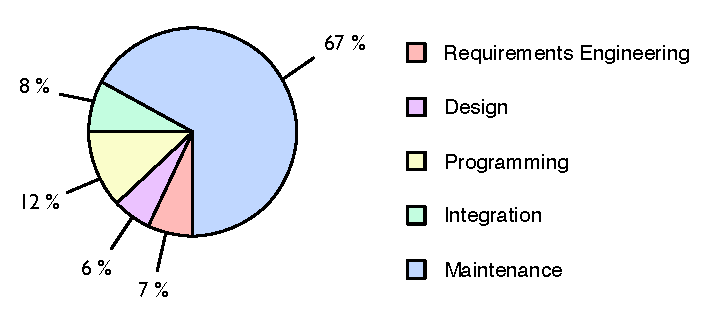
\includegraphics[width=0.7\textwidth]{./image/softwareLifeCycleCost.pdf}
      \caption{Ungefähre relative Kosten der Phasen des Software-Lebenszyklus
      (nach \cite{SoftwareEngineering} S. 11 und
      \cite{SoftwareLifeCycleModels})}
      \label{img:softwareLifecycleCost}
    \end{center}
  \end{figure}
  
  Es soll eine Konsolidierung statt finden, zwischen den 18 Soll-Kriterien und
  den wichtigen Aspekten im Software-Lebenszyklus für die \ac{ZKB}. Die
  Konsolidierung wird in der Tabelle \ref{tab:kosolidierungDerSollKriterien}
  gezeigt.
  
  \begin{table}[!h]
    \sffamily 
    \begin{center}
      \begin{threeparttable}
        \begin{tabular}{p{9cm}cccc}
          \toprule
          Anforderung & (Si) & (Ko) & (Re) & (Im)\\
          \midrule
          \ref{itm:Soll-01} & ++ &    &    &    \\
          \ref{itm:Soll-02} & +  &    &    &    \\
          \ref{itm:Soll-03} &    & ++ &    &    \\
          \ref{itm:Soll-04} &    & +  &    &    \\
          \ref{itm:Soll-05} &    &    &    &    \\
          \ref{itm:Soll-06} & +  & ++ &    & ++ \\
          \ref{itm:Soll-07} &    &    &    &    \\
          \ref{itm:Soll-08} &    &    &    &    \\
          \ref{itm:Soll-09} &    &    &    &    \\
          \ref{itm:Soll-10} &    &    &    &    \\
          \ref{itm:Soll-11} &    &    &    &    \\
          \ref{itm:Soll-12} &    & ++ &    &    \\
          \ref{itm:Soll-13} &    &    & ++ &    \\
          \ref{itm:Soll-14} &    & +  &    &    \\
          \ref{itm:Soll-15} &    &    &    &    \\
          \ref{itm:Soll-16} &    &    &    &    \\
          \ref{itm:Soll-17} &    &    & +  &    \\
          \ref{itm:Soll-18} &    &    &    & ++ \\
          \bottomrule
        \end{tabular}
        \caption{Wie wichtig sind die Soll-Kriterien für die ZKB.}
        \label{tab:kosolidierungDerSollKriterien}
        \medskip 
        %\footnotesize\textbf{Legende:}\smallskip 
        \begin{tablenotes}[++]\footnotesize 
          \item[(Si)] Sicherheit 
          \item[(Ko)] Kosten in der Maintenance Phase des Software-Lebenszyklus
          \item[(Re)] Ressourcen 
          \item[(Im)] Image
          \item[++] hat grossen Einfluss
          \item[+] hat Einfluss
        \end{tablenotes} 
      \end{threeparttable}
    \end{center}
  \end{table}
  
  Die Soll-Kriterien mit zwei oder mehr + werden als ``wichtig'', mit einem
  + als ``nice to have'' und ohne + als ``nicht wichtig'' priorisiert.
  
  \subsection{Wichtig}
  
  \begin{description}
  \item[Soll-01 - Zugriffskontrolle 
  (Authentifizierung/Authorisation/Rollenverwaltung)]
  Auf die Sicherheit von Applikationen in einer Bank wird grossen Wert
  gelegt. Mit einer genügenden Authentifizierung, Authorisation und
  Rollenverwalung, kann eine Applikation sicher implementiert werden.
  
  \item[Soll-03 - Modulare Architektur]
  Um wärend der Maintenance-Phase des Software-Lebenszyklus notwendige
  Anpassungen an einer Applikation machen zu können, ist eine modulare
  Architekur von grossem Vorteil. Zudem ist das auch wärend der
  Entwicklungs-Phase hilfreich.
  
  \item[Soll-06 - Testing]
  Um wärend der Maintenance-Phase des Software-Lebenszyklus notwendige
  Anpassungen an einer Applikation machen zu können, ist ein gutes Testing von
  grossem Vorteil. Das Testing hat auch einen grossen Einfluss auf das Image,
  denn wer möchte schon fehlerhafte Software verwenden. Durch eine gute
  Testbasis, kann auch die Sicherheit einer Applikation gesteigert werden.
  
  \item[Soll-12 - Dokumentation]
  Eine saubere und verständliche Dokumentation eines Web Application Frameworks
  ist das A und O um während allen Software-Lebenszyklen effizient arbeiten zu
  können. Ein Web Application Framework mit einer brillianten Dokumentation hat
  bestimmt höhere Chancen sich längerfristig am Markt durchzusetzten.
  
  \item[Soll-13 - Community]
  Damit die notwendigen Ressourcen, für die Umsetztung und Wartung eines
  Software-Projekts gefunden werden, wird eine entsprechend grosse Community
  benötigt. Wenn die Community genügend gross ist, kann man davon ausgehen,
  dass auch in der Zukunft noch genügend Ressourcen in diesem Bereich
  erreichbar sind.
  
  \item[Soll-18 - AJAX-Unterstützung]
  In der Zeit von Google Mail, Facebook und Twitter wird die Verwendung von
  \ac{Ajax} unterstützten Web Applikationen zur Gewohnheit. Um mit einer Web
  Applikation ein zeitgemässes, flexibles und innovatives Image vermitteln zu
  können, sollten diese mit Ajax-Unterstütztung gebaut werden.
  
  \end{description}
  
  \subsection{Nice to have}
  
  \begin{description}
  \item[Soll-02 - Form-Validierung]
  Eine saubere Form-Validierung gehört zu den notwendigen Werkzeugen, um eine
  sichere Web Applikation zu entwickeln. Dennoch kann durch gutes Testing und
  eine sichere Zugriffskontrolle der selbe Effekt erzielt werden.
  
  \item[Soll-04 - Schnittstellen und Webservices]
  Durch die breite Unterstützung von Schnittstellen und Webservice Technologien
  in der Java Welt, muss ein Web Framework dies nicht schon von Haus aus
  mitbringen. Fall es doch vorhanden ist, um so besser.
  
  \item[Soll-14 - IDE-Unterstuetzung]
  Eine IDE-Unterstützung ist zu präferieren, soll aber kein Hinderniss für den
  Einsatz eines guten Web Frameworks sein.
  
  \item[Soll-17 - Lernkurve fuer EntwicklerInnen]
  Durch die Unterstützung einer soliden Community und einer guten Dokumentation
  kann die Lernkurve beträchtlich beeinflusst werden.
  
  \end{description}
  
  \subsection{Unwichtig}
  
  \begin{description}
  \item[Soll-05 - MVC-Entwurfsmuster]
  Das \ac{MVC} Konzept ist sicher gut, sollte aber nicht eine Anforderung an ein
  Web Framework sein, da es ebenbürdige Alternativen gibt, eine nennenswerte währe
  \ac{MVP}.
  
  \item[Soll-07 - Internationalisierung und Lokalisierung]
  Die \ac{ZKB} hat ihr Geschäftsfeld im Kanton Zürich. Somit ist eine
  Internationalisierung und Lokalisierung nicht wirklich nötig. Da die \ac{ZKB}
  im Auftrag des Kantons handelt, gehe ich davon aus, dass sich das nicht so
  schnell ändern wird.
  
  \item[Soll-08 - Object Relational Mapping (ORM)]
  In der Java Welt git es viele \ac{ORM} Lösungen, welche sich in den Jahren
  durchgesetzt haben, ein paar nennenswerte sind Hibernate, TopLink und
  EclipseLink. Da es Sache des Applikationsservers ist, welches \ac{ORM}
  verwendet wird, stellt dies keine Anforderung an ein Java Web Framework.
  
  \item[Soll-09 - Scaffolding / Rapid Prototyping]
  Mit Scaffolding und Rapid Prototyping kann in der Programmier-Phase des
  Software-Lebenszyklus die Arbeit erleichtert werden. In der Maintenance-Phase
  ergibt sich daraus kein Benefit.
  
  \item[Soll-10 - Caching]
  Caching kann bei Webseiten mit viel statischen Content die Datenmenge, die
  übertragen wird, enorm reduzieren. Bei Business-Applikationen, die über eine
  Rollenverwaltung verfügen, sind die Daten die übertragen werden, meistens sehr
  individuell. Somit besteht keine Nachfrage nach Caching
  
  \item[Soll-11 - View-Engine]
  Da Java eine Objekt Orientierte Sprache ist, wird das schon von der Sprache
  her unterstützt.
  
  \item[Soll-15 - Kosten fuer Entwicklungswerkzeuge]
  Die Kosten der Entwicklungswerkzeuge haben keinen Einfluss auf die
  Maintenance-Phase des Software-Lebenszyklus. Zudem gibt es genügend \acp{IDE}
  für Java, die Open Source sind. Ein Paar nennenswerte sind Eclipse, NetBeans
  und IntelliJ.
  
  \item[Soll-16 - Eignung fuer agile Entwicklung]
  Die Ansätze von Scrum und extreme Programming werden in der \ac{ZKB} je länger
  je mehr angewendet. Dennoch hat das keinen Einfluss auf die Maintenance-Phase
  des Software-Lebenszyklus.
  
  \end{description}
  
  \section{KO-Kriterien die nicht beachtet werden sollen}
  
  Damit die Durchführung der Evaluation einen Sinn ergibt, sollen einige
  KO-Kriterien nicht beachtet werden. In Absprache mit dem Fachbetreuer der
  \ac{ZKB} betrifft das folgende KO-Kriterien, die im Rahmen der Diplomarbeit
  nicht berücksichtigt werden:
  
  \begin{itemize}
    \item \ref{itm:KO-09} - Für Java-Applikationen (Internet, Extranet und
    Intranet) wird das ZIP-Framework eingesetzt.
    \item \ref{itm:KO-16} - Die Internet-Applikationen funktionieren auch
    eingeschränkt, ohne dass die Skript-Funktion im Browser aktiviert ist.
    \item \ref{itm:KO-20} - Für Ultra Thin Clients bzw. Browser-basierende
    Applikationen muss das aktuelle, Struts-basierende HTML-Client-Framework
    der ZKB Internet Plattform verwendet werden.
  \end{itemize}
  
  \section{Auswahl der Java Web Frameworks}
  
  Es sollen vier Java Web Frameworks für die Evaluation ausgewählt werden. Ein
  Java Web Framework, das in Frage kommt, wird Alternative genannt. Jede
  Alternative wird mit einer ID in der Form \{A\}-\{Laufnummer\} versehen.
  
  \subsection{Begründung}
  
  Es soll für jede Alternative der Grund der Wahl erläutert werden. In Absprache
  mit dem Projektbetreuer sollen aus den verschiednen Typen von Java Web
  Frameworks jeweils eines gewählt werden. Es wurden folgende Typen definiert:
  
  \begin{itemize}
    \item \ac{RIA} - Frameworks
    \item MVC - Frameworks
    \item Java Script/HTML/CSS - Cross-Compiler Frameworks
    \item In der \ac{ZKB} bereits eingesetzte Frameworks
  \end{itemize}
  
  \subsubsection{A-1 - ULC, Canoo RIA Suite}
  
  ULC, Canoo RIA Suite zählt zu den \ac{RIA} Frameworks. Gemäss Kick-off
  Protokoll Beschluss soll dieses Framework als Alternative gewählt werden.
  Zudem wird die ULC, Canoo RIA Suite in den schweizer Banken Credit Suisse und
  UBS eingesetzt.
  
  \subsubsection{A-2 - Struts 1.3.10 mit ZIP-Framework}
  
  MVC - Framework, das in der ZKB bereits eingesetzt wird.
  
  \subsubsection{A-3 - Vaadin 6.5.7}
  
  Vaadin zählt zu den Java Script/HTML/CSS - Cross-Compiler Frameworks und baut
  auf \ac{GWT} auf.
  
  \subsubsection{A-4 - Apache Wicket 1.4.17}
  
  Ein Framework das in der ZKB bereits eingesetzt wird. An dieser Stelle ist zu
  erwähnen, dass der Einsatz aufgrund von Ausnahmegenehmigungen eingesetzt
  werden darf. Diese müssten im Falle einer erfolgreichen Evaluation ebenfalls
  beantragt werden.
  
  \section{Prüfen der zu beachtenden KO-Kriterien}
  
  Es soll eine Prüfung aller Frameworks statt finden, ob es gegen definierte
  KO-Kriterien verstösst. Falls das der Fall ist, wird das Framework von der
  Evaluation ausgeschlossen. In Absprache mit dem Fachbetreuer der \ac{ZKB} gibt
  es gewisse KO-Kriterien, die im Rahmen der Diplomarbeit ausser Kraft treten,
  diese sollen nicht beachtet werden.

  \subsection{A-1 - ULC, Canoo RIA Suite}
  
  Leider wurde wärend der Analyse festgestellt, dass die ULC, Canoo RIA Suite
  nur in einer Java Virtual Machine\footnote{Die Java Virtual Machine ist der
  Teil der \ac{JRE}, der für die Ausführung des Java-Bytecodes verantwortlich
  ist, siehe \cite{JavaVirtualMachine}.} lauffähig ist. Das wird über die
  Technik von Java-Web-Start\footnote{Java-Web-Start ist eine Technik von
  Oracle (damals entwickelt von Sun Microsystems), die es ermöglicht, Java-Anwendungen
  über das Internet mit nur einem Klick zu starten. Im Unterschied zu
  Java-Applets benötigen Java-Web-Start-Anwendungen keinen Browser, um ablaufen
  zu können, siehe \cite{JavaWebStart}.} oder mit der Hilfe von einem
  Java-Applet\footnote{Ein Java-Applet ist ein Computerprogramm, das in der
  Programmiersprache Java verfasst wurde und normalerweise in einem Webbrowser
  ausgeführt wird, siehe \cite{JavaApplet}.} vollbracht. Das ist ersichtlich im
  ULC Architektur Guide, siehe \cite{ULCArchitectureGuide} S. 18. Damit
  verstösst diese Alternative gegen die KO-Kriterien \ref{itm:KO-18} und
  \ref{itm:KO-19}. Aufgrund des Vorgehens aus der Abbildung
  \ref{img:ablaufEvaluation} wird diese Alternative aus der Evaluation
  ausgeschlossen.
  
  Der Client könnte auch als standalone Client implementiert oder in einen
  bestehenden Client integriert werden. Das nützt nichts, da diese Situation
  bereits mit den Java Swing Clients besteht, und abgelöst werden soll.
  
  Falls sich die Grundsätze der IT-Architektur der \ac{ZKB} in der Zunkunft
  dahingehend ändern, dass Java Web Start oder Java Applets verwendet werden
  dürften, stellt die ULC, Canoo RIA Suite ein gute Alternative zur Ablösung
  bestehender Swing Applikationen.
  
  \subsection{A-2 - Struts 1.3.10 mit ZIP-Framework}
  
  Es wurde keine KO-Kriterien gefunden, die für diese Alternative zutreffen.
  
  \subsection{A-3 - Vaadin 6.5.7}
  
  Es wurde keine KO-Kriterien gefunden, die für diese Alternative zutreffen.

  \subsection{A-4 - Apache Wicket 1.4.17}
  
  Es wurde keine KO-Kriterien gefunden, die für diese Alternative zutreffen.
    
  \section{Gewichtete Nutzwertanalyse mit dem Analytic Hirarchy Process}
  
  Es sollen die Soll-Kriterien, auf welche die Frameworks verglichen werden,
  bestimmt werden. Danach soll nach der Methode des \ac{AHP} die Gewichtung der
  Soll-Kriterien vorgenommen und, zur Berechnung der Nutzwertanalyse,
  verwendet werden. Für jede mögliche Alternative soll der Erfüllungsgrad der
  Soll-Kriterien bestimmt und, zur Berechnung der Nutzwertanalyse, vewendet
  werden. Das Resultat der Nutzwertanalyse soll dargestellt werden.
  
  \subsection{Bestimmen der Kriterien}
  
  Die Kriterien, welche in die Evaluation miteinbezogen werden, und somit für
  jede Alternative untersucht werden soll, sind die ``wichtigen''
  Soll-Kriterien:
  
  \begin{itemize}
    \item Soll-01 - Zugriffskontrolle 
    (Authentifizierung/Authorisation/Rollenverwaltung)
    \item Soll-03 - Modulare Architektur
    \item Soll-06 - Testing
    \item Soll-12 - Dokumentation
    \item Soll-13 - Community
    \item Soll-18 - AJAX-Unterstützung
  \end{itemize}
  
  \subsection{Bestimmen der Gewichte mit dem Analytic Hirarchy Process}
  
  Die Bestimmung der Gewichte wird über die Methode des \ac{AHP} gemacht. Für
  den Vergleich der Soll-Kriterien wird die Frage - \begin{itshape}``Wie
  wichtig ist das Soll-Kriterium für die \ac{ZKB}?''\end{itshape} - gestellt.
  
  Es werden alle ``wichtigen'' Soll-Kriterien miteinander verglichen. Die
  Vergleichsmatrix und die daraus resultierende Gewichtung ist in der Tabelle
  \ref{tab:gewichtungDerSollKriterien} und der Abbildung
  \ref{img:gewichtungSollKriterien} ersichtlich. Für die Werte in der
  Vergleichsmatix wird die Skala der Vergleichsgrad, siehe Tabelle
  \ref{tab:vergleichsgrade}, verwendet.
  
  Um die Gewichte anhand der erstellten Vergleichsmatix zu berechnen, wird das
  Java Programm JAHP 2.1 verwendet.
  
  Der Inkonsistenzfaktor beträgt 0.04754 und ist somit sehr klein. Die
  getroffenen Annahmen der Gewichtung sollten desshalb aussagekräftig sein.
  \newline
  
  \begin{table}[!h]
    \sffamily 
    \begin{center}
      \begin{tabular}{l|cccccc|r}
        \toprule
        Vergleich & Soll-01 & Soll-03 & Soll-06 & Soll-12 & Soll-13 & Soll-18
        & Gewichtung\\
        \midrule
        Soll-01 & 1 & 5 & 3 & 5 & 5 & 3 & 34.81 \%\\
        Soll-03 & $\frac{1}{5}$ & 1 & $\frac{1}{3}$ & 1 & 1 & $\frac{1}{5}$ &
        5.91 \%\\
        Soll-06 & $\frac{1}{3}$ & 3 & 1 & 3 & 3 & 1 & 17.93 \%\\
        Soll-12 & $\frac{1}{5}$ & 1 & $\frac{1}{3}$ & 1 & $\frac{1}{3}$ &
        $\frac{1}{5}$ & 4.85 \% \\
        Soll-13 & $\frac{1}{5}$ & 1 & $\frac{1}{3}$ & 3 & 1 & $\frac{1}{5}$ &
        9.07 \%\\ Soll-18 & $\frac{1}{3}$ & 5 & 1 & 5 & 5 & 1 & 27.43 \%\\
        \bottomrule
      \end{tabular}
      \caption{Vergleichsmatrix der Soll-Kriterien nach der Methode des AHP.}
      \label{tab:gewichtungDerSollKriterien}
    \end{center}
  \end{table}
  
  \begin{figure}[ht]
    \begin{center}
      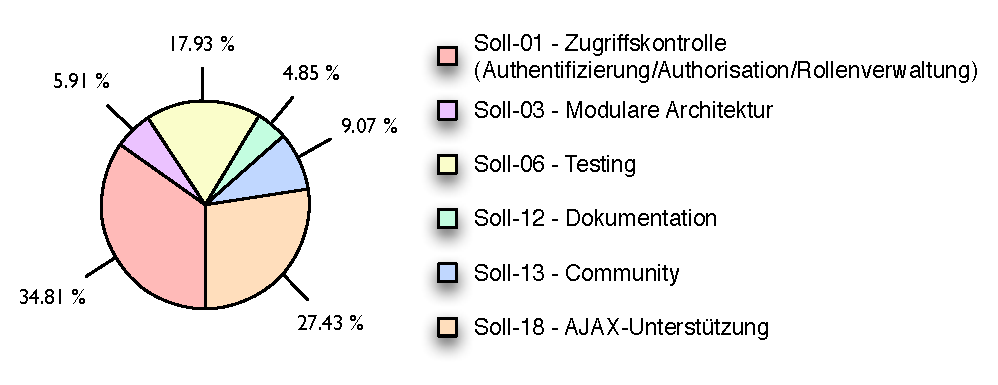
\includegraphics[width=0.95\textwidth]{./image/gewichtungSollKriterien.pdf}
      \caption{Gewichtung der Soll-Kriterien nach der Methode des AHP}
      \label{img:gewichtungSollKriterien}
    \end{center}
  \end{figure}
  
  \subsection{Bestimmen des Erfüllungsgrades}
  
  Für die Werte zur Bestimmung der Erfüllungsgrade wird die Skala der
  Erfüllungsgrade, siehe Tabelle \ref{tab:erfuellungsgrade}, verwendet. Die
  Begründung der gegebenen Punkt wird für jeden Punkt erläutert.
  
  \subsection{A-1 - ULC, Canoo RIA Suite}
  
  Wurde aufgrund der KO-Kriterien \ref{itm:KO-18} und \ref{itm:KO-19} aus der
  Evaluation ausgeschlossen.
  
  \subsection{A-2 - Struts 1.3.10 mit ZIP-Framework}
  
  Das Ergebnis ist in der Tabelle \ref{tab:nwaA2} ersichtlich. Der Nutzwert
  liegt bei xx.xx.
  
  \begin{table}[ht]
    \sffamily 
    \begin{center}
      \begin{tabular}{l|rrr}
        \toprule
        Kriterien & Gewichtung \(g\) & Erfüllungsgrad \(e\) & Wertigkeit
        \(_A-_2\) \\
        \midrule
        Soll-01   & 34.81 \% & x & y \\
        Soll-03   &  5.91 \% & x & y \\
        Soll-06   & 17.93 \% & x & y \\
        Soll-12   &  4.85 \% & x & y \\
        Soll-13   &  9.07 \% & x & y \\
        Soll-18   & 27.43 \% & x & y \\
        \midrule
        \midrule
        Ergebnis  & 100.00 \% &   & z \\
        \bottomrule
      \end{tabular}
      \caption{Nutzwertanalyse der Alternative A-2 - Struts 1.3.10 mit
      ZIP-Framework}
      \label{tab:nwaA2}
    \end{center}
  \end{table}
  
  \subsection{A-3 - Vaadin 6.5.7}
  
  Das Ergebnis ist in der Tabelle \ref{tab:nwaA3} ersichtlich. Der Nutzwert
  liegt bei 7.5654.
    
  \begin{table}[ht]
    \sffamily 
    \begin{center}
      \begin{tabular}{l|rrr}
        \toprule
        Kriterien & Gewichtung \(g\) & Erfüllungsgrad \(e\) & Wertigkeit
        \(_A-_3\) \\
        \midrule
        Soll-01   & 34.81 \% & 7 & 2.4367 \\
        Soll-03   &  5.91 \% & 5 & 0.2955 \\
        Soll-06   & 17.93 \% & 9 & 1.6137 \\
        Soll-12   &  4.85 \% & 8 & 0.3880 \\
        Soll-13   &  9.07 \% & 4 & 0.3628 \\
        Soll-18   & 27.43 \% & 9 & 2.4687 \\
        \midrule
        \midrule
        Ergebnis  & 100.00 \% &   & 7.5654 \\
        \bottomrule
      \end{tabular}
      \caption{Nutzwertanalyse der Alternative A-3 - Vaadin 6.5.7}
      \label{tab:nwaA3}
    \end{center}
  \end{table}
  
  \subsubsection{Soll-01 - Zugriffskontrolle - 7 Punkte}
  
  Vaadin biete keine Unterstützung für Authentifizierung und Autorisierung an.
  Es gibt ein alternatives Projekt, das sich
  vaadin-appfoundation\footnote{Projektinformationen sind hier zu finden:
  \url{http://code.google.com/p/vaadin-appfoundation/}} nennt. Dieses Projekt
  beinhaltet ein Authorisierungs Modul, mit dem ein Rollenkonzept implementiert
  werden kann.
  
  \noindent
  Vaadin behauptet von sich, eines der sichersten Web Frameworks zu sein.
  \newline
  
  \begin{itshape}``The server-side architecture of Vaadin is immune to the usual
  risks affecting many other RIA frameworks. Your business logic and UI state
  are kept securely on the server, and never sent to the browser where it could
  be analyzed by a potential attacker. Vaadin doesn't even trust the components
  or the RPC model of GWT, which is used to render the UI.

  In addition, we have implemented several other security mechanisms in Vaadin
  to prevent eg. man-in-the-middle and cross-site scripting
  attacks.''\end{itshape}
  \footnote{Siehe \cite{VaadinSecurityAlerts}}
  \newline
  
  \noindent
  Zwei Punkte abzug, da keine Rollenverwaltung vorhanden ist.
  
  \subsubsection{Soll-03 - Modulare Architektur - 5 Punkte}
  
  Vaadin bietet ein eigenes Add-on Repository an, unter welchem Erweiterungen
  zum Framework bezogen werden können. Das deutet auf eine modulare Architektur
  hin. Wie modular die Architektur wirklich ist, konnte ich nach meinem Research
  nicht genau abschätzen.
  
  Desshalb gibt es nur fünf Punkte.
  
  \subsubsection{Soll-06 - Testing - 9 Punkte}
  
  Für das Framework steht eine komplette Test Suite namens TestBench zur
  Verfügung. Mit TestBench können UI Regressionstest aufgezeichnet und
  automatisiert durchgeführt werden. TestBench ist eine kostenpflichtige
  Extension zu Vaadin. Das ganze basiert auf Selenium, einem Open Source
  Projekt zur Abwicklung von Tests im Web-Umfeld, und JUnit, einem Open Source
  Projekt zur Abbildung von Unit Tests.
  
  Da ein Test Framework existiert, das auf aktuellen Techniken basiert, gibt es
  die maximale Punktzahl.
  
  \subsubsection{Soll-12 - Dokumentation - 8 Punkte}
  
  Die Entwickler haben sogleich ein komplettes Buch zum Framework mit vielen
  hilfreichen Beispielen geschrieben. Das Buch ist in HTML oder als PDF frei
  verfügbar und kostenlos. Es enthält alle wichtigen Informationen, welche zur
  Entwicklung nötig sind. Auf Amazone gibt es nur ein weiteres Buch, das sich
  diesem Framework gewidmet hat, das ist aber nicht weiter schlimm, da das
  Framework relativ neu ist.
  
  Die Dokumentation wird auf der Website mit einer Menge von Tutorials
  abgerundet. Es existieren auch die üblichen Dinge, wie das JavaDoc zum
  \ac{API}, die Hinweise auf die Lizenz, \ac{FAQ} und vieles mehr. Das alles
  wirk sehr sauber, schön und vollständig.
  
  Leider existiert die Dokumentation nur auf Englisch, desshalb gibt es einen
  Punkt Abzug.
  
  \subsubsection{Soll-13 - Community - 4 Punkte}
  
  Das Framework Vaadin ist unter seinem Namen noch nicht sehr lange bekannt,
  früher wurde es unter dem Namen IT Mill entwickelt. Das kann zu einem leicht
  falschen Resultat führen, wenn man die Community nach Vaadin untersucht.
  
  Laut ohloh\footnote{ohloh ist eine Community Plattform für
  Softwareentwickler, siehe \url{http://www.ohloh.net/}} gibt es 183 User, die
  Vaadin verwenden und 62 Contributer.
  
  Bei DZone\footnote{Eine weitere Community Plattform für Softwareentwickler,
  siehe \url{http://www.dzone.com/}} findet man 75 Posts, welche sich direkt mit
  Vaadin befassen
  
  Die Community für Vaadin ist gerade dabei sich zu bilden und noch nicht sehr
  stark, somit sind es nur 4 Punkte.

  \subsubsection{Soll-18 - AJAX-Unterstützung - 9 Punkte}
  
  \ac{Ajax} wird massiv unterstützt. Alle \ac{UI} Aktionen basieren auf diesem
  Prinzip. Zudem kann eine Javascript Library wie JQuery oder Prototype
  integriert werden. Desshalb gibt es die maximale Punktzahl.
  
  \subsection{A-4 - Apache Wicket 1.4.17}
  
  Das Ergebnis ist in der Tabelle \ref{tab:nwaA4} ersichtlich. Der Nutzwert
  liegt bei xx.xx.
  
  \begin{table}[ht]
    \sffamily 
    \begin{center}
      \begin{tabular}{l|rrr}
        \toprule
        Kriterien & Gewichtung \(g\) & Erfüllungsgrad \(e\) & Wertigkeit
        \(_A-_4\) \\
        \midrule
        Soll-01   & 34.81 \% & x & y \\
        Soll-03   &  5.91 \% & x & y \\
        Soll-06   & 17.93 \% & x & y \\
        Soll-12   &  4.85 \% & x & y \\
        Soll-13   &  9.07 \% & x & y \\
        Soll-18   & 27.43 \% & x & y \\
        \midrule
        \midrule
        Ergebnis  & 100.00 \% &   & z \\
        \bottomrule
      \end{tabular}
      \caption{Nutzwertanalyse der Alternative A-4 - Apache Wicket 1.4.17}
      \label{tab:nwaA4}
    \end{center}
  \end{table}

  \section{Resultat} 
  
  \cleardoublepage
  
  % ===========================================================================
  % Kapitel XXX beginns here
  % ===========================================================================
   
  \chapter{Integration in die ZKB Infrastruktur
  möglich?}\label{chapter:IntegrationInDieZkbInfrastrukutr}
  
  In diesem Kapitel soll behandelt werden, ob eine Integration der jeweiligen Java
Web Frameworks in die Infrastruktur der \ac{ZKB} möglich ist. Dabei soll geprüft
werden, ob die notwenigen \acp{API}, auf welchen die Frameworks aufbauen, durch
die zur Verfügung gestellten Applikationsserver, abgedeckt sind. Als Grundlage
werden die Informationen aus dem Kapitel
\ref{chapter:InfrastrukturDerZuercherKantonalbank}
(\nameref{chapter:InfrastrukturDerZuercherKantonalbank}, S.
\pageref{chapter:InfrastrukturDerZuercherKantonalbank}ff) verwendet.

Es wird auf die Prüfung vom Framework ``A1 - ULC, Canoo RIA Suite'' verzichtet,
da es aufgrund der Evaluation als mögliche Alternative entfällt.

\section{A2 - Struts 1.3.10 mit ZIP-Framework}

Das Framework ``A2 - Struts 1.3.10 mit ZIP-Framework'' kann in die bestehende
Infrastruktur der \ac{ZKB} integriert werden. Für den Betrieb einer Struts
Applikation ist ein Servlet Container notwendig, dieser wird in der
Infrastruktur mit dem JBoss Web, welcher auf Apache Tomcat 6.0 basiert, zur
Verfügung gestellt. Die genauen Anforderungen an die Konfiguration können aus
der Dokumentation entnommen werden, siehe \cite{StrutsDokumentation}.

Das Framework ist zudem in der \ac{ZKB} schon im Einsatz. Eine Applikation,
welche damit entwickelt wurde, ist das Online-Banking, auch genannt ``OnBa''.

\section{A3 - Vaadin 6.5.7}

Das Framework ``A3 - Vaadin 6.5.7'' kann in die bestehende
Infrastruktur der \ac{ZKB} integriert werden. Der Betrieb setzt ebenfalls ein
Servlet Container voraus. In der Dokumentation ist zu entnehmen, dass es sich
dabei mindestens um einen Apache Tomcat 6.0 handelt, siehe \cite{BookOfVaadin}
S. 11. Als Laufzeitumgebung wird mindestens Java 1.5 vorausgesetzt, was
ebenfalls verfügbar ist.

Das Framework wurde in der \ac{ZKB} noch nie eingesetzt. Der Einsatz müsste mit
den aktuellen Bestimmungen aus der IT Architektur über einen Ausnahmegenehmigung
geregelt werden.

\section{A4 - Apache Wicket 1.4.17}

Das Framework ``A4 - Apache Wicket 1.4.17'' kann in die bestehende IT
Infrastruktur der \ac{ZKB} integriert werden. Für den Betrieb einer Struts
Applikation ist auch nur ein Servlet Container notwendig, siehe
\cite{WicketDokumentation}.

Das Framework ist ebenfalls bereits in der \ac{ZKB} im Einsatz. Der Einsatz
wurde durch eine Ausnahmegenehmigung geregelt. Eine Applikation, welche damit
entwickelt wurde, ist das Bond-Rating-Tool, auch genannt ``BoReTo''.

\section{Resultat}

Alle drei evaluierten Java Web Frameworks entsprechen den Begebenheiten aus der
\ac{ZKB} IT Infrastruktur und sind somit für den Einsatz geeigent. Namentlich
sind das folgende:

\begin{itemize}
  \item Struts 1.3.10 mit ZIP-Framework
  \item Vaadin 6.5.7
  \item Apache Wicket 1.4.17
\end{itemize}

  \cleardoublepage

  % ===========================================================================
  % Kapitel XXX beginns here
  % ===========================================================================
   
  \chapter{Implementierung der gefundenen Swingkomponenten
  möglich?}\label{chapter:ImplementierungDerGefundenenSwingkomponenten}
  
  In diesem Kapitel soll behandelt werden, ob eine Implementierung, der im Kapitel 
\ref{chapter:AnalyseDerJavaSwingApplikationen}
(\nameref{chapter:AnalyseDerJavaSwingApplikationen}, S.
\pageref{chapter:AnalyseDerJavaSwingApplikationen}ff) gefundenen Java Swing
Komponenten, äquivalent möglich ist. Dabei sollen die Dokumentationen und
Tutorials, welche für die Frameworks vorhanden sind, als Grundlage dienen. Die
Prüfung soll durch einen visuellen Vergleich statt finden, ob die 32 gefundenen
Komponenten und die sieben gefundenen GUI Paradigmen abgedeckt sind. Das
Resultat soll in Form einer Tabelle mit dem jeweiligen Abdeckungsgrad
dargestellt werden.

Es wird auf die Prüfung der Komponenten vom Framework ``A1 - ULC, Canoo RIA
Suite'' verzichtet, da es aufgrund der Evaluation als mögliche Alternative
entfällt.

\section{A2 - Struts 1.3.10 mit ZIP-Framework}

\section{A3 - Vaadin 6.5.7}

In der Dokumentation zu Vaadin gibt es eine komplette Übersicht aller
unterstützten Komponenten, siehe \cite{VaadinKomponenten}. Diese können online
mit einem Browser betrachtet und auf deren Usability ausprobiert werden.
Folgende Komponenten werden unterstützt:

\begin{itemize}
  \item Es werden alle Top-Level Komponenten unterstützt
  \item Es werden alle Intermediate-Komponenten unterstützt
  \item Es werden alle Atomic-Komponenten bis auf das
  \(JFormattedTextField\) unterstützt.
  \item Es werden alle speziellen Komponenten bis auf
  \(JFreeChart\) unterstützt. Dafür gibt es ein offizielles
  Add-on mit dem Namen ``JFreeChart wrapper for Vaadin'', welches die
  Unterstützung von \(JFreeChart\) in den Formaten \ac{PNG} und \ac{SVG}
  sichert.
  \item Die ``Neuen'' Komponenten können alle implementiert werden. Das
  Akkordeon und der Zeit-Panel werden schon von Haus aus unterstützt.
\end{itemize}

\noindent
Folgende Design-Patterns werden unterstützt:

\begin{itemize}
  \item Das MVC-Pattern wird unterstützt
  \item Das Observer-Pattern wird unterstützt
  \item Tabellen-Filter werden unterstützt
  \item Duch die Unterstützung von Ajax ist das Worker-Pattern abgedeckt.
\end{itemize}

\noindent
Es werden alle Komponenten bis auf das \(JFormattedTextField\) und
\(JFreeChart\)\footnote{Es ist zu bedenken, dass für das \(JFreeChart\) ein
Add-on existiert, diese Komponente wurde nicht in die Abdeckung
miteingerechnet.} unterstützt, das ist eine Abdeckung von 93.75\%. Es werden
alle GUI Paradigmen unterstützt, das ist eine Abdeckung von 100.00\%.

\section{A4 - Apache Wicket 1.4.17}

\section{Resultat}

In der Tabelle \ref{tab:unterstuetztungDerKomponenten} wird die Abdeckung der
unterstützten Komponenten und GUI Paradigmen dargestellt.
\newline

\begin{table}[!h]
  \sffamily 
  \begin{center}
    \begin{tabular}{lrr}
      \toprule
      \textbf{Java Web Framework} & \textbf{GUI Komponenten} & \textbf{GUI
      Paradigmen}\\
      \midrule
      A1 - ULC, Canoo RIA Suite & Prüfung entfällt & Prüfung entfällt\\
      A2 - Struts 1.3.10 mit ZIP-Framework & xx.xx\% & xx.xx\%\\
      A3 - Vaadin 6.5.7 & 93.75\% & 100.00\%\\
      A4 - Apache Wicket 1.4.17 & xx.xx\% & xx.xx\%\\
      \bottomrule
    \end{tabular}
    \caption{Abdeckungsgrad der gefundenen GUI Komponenten und Paradigmen}
    \label{tab:unterstuetztungDerKomponenten}
  \end{center}
\end{table}

  \cleardoublepage
  
  % ===========================================================================
  % Kapitel XXX beginns here
  % ===========================================================================  
  
  \chapter{Proof of Concept - Umsetzung durch einen
  Prototypen}\label{chapter:ProofOfConcept}
  
  In diesem Kapitel sollen die Anforderungen und Akzeptanztests für einen
Prototypen definiert werden. Als Grundlage sollen die Komponenten und
Verhaltensmuster der Applikation Strukti Live 1.2 dienen, da die Applikation
öffentlich verfügbar ist.

Wie im Kapitel \ref{chapter:MethodenZurEntscheidungsfindungBeiEinerEvaluation}
(\nameref{chapter:MethodenZurEntscheidungsfindungBeiEinerEvaluation}, S.
\pageref{chapter:MethodenZurEntscheidungsfindungBeiEinerEvaluation}ff)
beschrieben, gilt der Proof of Concept als erfolgreich, wenn alle
Akzeptanztests erfolgreich abgenommen wurden. Die Abnahme der Akzeptanztests
erfolgt durch eine visuelle Prüfung.

\section{Anforderungen mit User Stories}

\begin{description}
\item[US-1\label{itm:US-1}]
Es soll das Fenster in sechs Teile (Panels) aufgeteilt werden. Die Aufteilung
soll in drei Spalten und zwei Zeilen aufgeteilt werden, wobei die erste Zeile
eine Höhe von 150px\footnote{px ist die Abkürzung für Pixel, zu Deutsch
Bildpunkt. Ein Pixel bezeichnet die kleinste Einheit einer digitalen
Rastergrafik.} und die zweite Zeile eine höhe von 606px haben soll.

\item[US-2\label{itm:US-2}]
Es soll die erste und die dritte Spalte eine Breite von 220px und die zweite
und mittlere Spalte eine Breite von 552px haben.

\item[US-3\label{itm:US-3}]
Es soll der Panel in der ersten Zeile und der ersten Spalte immer ein Logo der
Applikation dargestellt werden. Wenn mit der linken Maustaste auf das Bild
``geklickt'' wird, soll die Startansicht geladen werden.

\item[US-4\label{itm:US-4}]
Es soll der Panel in der ersten Zeile und der zweiten Spalte der Hintergrund
hellblau eingefärbt werden. In der linken unteren Ecke des Panels soll der Titel
der aktuellen Ansicht angezeigt werden.

\item[US-5\label{itm:US-5}]
Es soll der Panel in der zweiten Zeile und der ersten Spalte als
Navigationspanel dienen. Die verschiedenen Ansichten sollen über den
Navigationspanel angesteuert werden können.

\item[US-6\label{itm:US-6}]
Der Navigationspanel soll eine zweistufige Navigation anbieten. Ansichten,
welche Gruppiert werden können, sollen in der zweiten Stufe untergebracht
werden. Navigationen, welche sich in der zweiten Stufe befinden, sollen
unterhalb der übergeordneten Navigationen eingeruckt dargestellt werden.

\item[US-7\label{itm:US-7}]
Die aktuell angesteuerte Ansicht soll im Navigationspanel andersfarbig
dargestellt werden.

\item[US-8\label{itm:US-8}]
Im Navigationspanel sollen die verschiednen Navigationspunkte auf der ersten
Stufe über ein Separator visuell voneinander getrennt werden.

\item[US-9\label{itm:US-9}]
Wenn ein Navigationspunkt der ersten Stufe im Navigationspanel ``angeklickt''
wird, sollen die darunter liegenden zweitstufigen Navigationspunkt sichtbar
werden.

\item[US-10\label{itm:US-10}]
Es sollen zwei Navigationen auf der ersten Stufen angezeigt werden. Die
Navigationen sind ``Einführung'' und ``Produktauswahl''.

\item[US-11\label{itm:US-11}]
Es sollen zwei Navigationen auf der zweiten Stufen unterhalb der Navigation
``Produktauswahl'' angezeigt werden. Die Navigationen sind
``Produktbeschreibung'' und ``Produktdesign''.

\item[US-12\label{itm:US-12}]
Wenn der Navigationspunkt ``Einführung'' ausgewählt wird, soll in der zweiten
Reihe und der zweiten Spalte ein Einführungstext zum Proof of Concept
dargestellt werden.

\item[US-13\label{itm:US-13}]
Wenn der Navigationspunkt ``Produktauswahl'' ausgewählt wird, soll in der
zweiten Reihe und der zweiten Spalte eine Buttonmatrix mit den Produkten
``Put Option'', ``Soft Runner'' und ``Protein'' dargestellt werden. Die
Navigationen ``Produktbeschreibung'' und ``Produktdesign'' sollen angezeigt
werden und deaktiviert sein.

\item[US-14\label{itm:US-14}]
Wenn der Navigationspunkt ``Produktauswahl'' ausgewählt wird, sollen in der
zweiten Zeile und der dritten Spalte Filteroptionen für die Produkte in der Form
von CheckBoxen dargestellt werden.

\item[US-15\label{itm:US-15}]
Wenn eine Filteroption gewählt wird, sollen die Produkte entsprechend des
Filters aktiv oder inaktiv gesetzt werden.

\item[US-16\label{itm:US-16}]
Wenn ein Produkt ausgewählt wird, dann soll in der zweiten Reihe und der zweiten
Spalte die Produktbeschreibung angezeigt werden. Die Produktbeschreibung
besteht aus einem Fliesstext und einem TabbedPanel welcher sechs Tabs hat:
``Eigenschaften'', ``Chancen \& Risiken'', ``Rückzahlungsmodus'',
``Beispiele'', ``Steuern'' und ``Klassifizierung''. Die Navigationspunkte
``Produktbeschreibung'' und ``Produktdesign'' sollen nun aktiv gesetzt werden.

\item[US-17\label{itm:US-17}]
Wenn ein Tab ausgewählt wird, sollen die entsprechenden Informationen zum
Produkt dargestellt werden.

\item[US-18\label{itm:US-18}]
Wenn der Navigationspunkt ``Produktdesign'' ausgewählt wird, soll das
Auszahlungsprofil eines möglichen Produkts dargestellt werden. Die notwendigen
Eckdaten sollen in der zweiten Zeile und der dritten Spalte in der Form von
Textfeldern oder Slidern dargestellt werden.

\item[US-19\label{itm:US-19}]
Wenn die Werte in den Textfeldern oder Slidern geändert werden, dann soll sich
das Auszahlungsprofil entsprechend anpassen.
\end{description}

\section{Priorisierung der User Stories}

Es werden alle UserStories als \begin{itshape}hoch\end{itshape} priorisiert.

\section{Akzeptanztests}

Für alle Akzeptanztests gilt als Voraussetzung, dass der Prototyp auf einem
Applikationsserver läuft. Die Akzeptanztest werden mit den Webbrowsern Chrome
und Safari durchgeführt, um sicherzustellen dass der Prototyp unabhängig vom
Webbrowser implementiert wurde.

\begin{description}
\item[T-1.1\label{itm:T-1.1}]
Die vorgegebenen Masseinheiten der Zeilen sollen mit einem Screenshot geprüft werden.

\item[T-2.1\label{itm:T-2.1}]
Die vorgegebenen Masseinheiten der Spalten sollen mit einem Screenshot geprüft werden.

\item[T-3.1\label{itm:T-3.1}]
Es soll geprüft werden, ob das Logo in der ersten Zeile und der ersten Spalte
vorhanden ist.

\item[T-3.2\label{itm:T-3.2}]
Mit einem Klick auf das Logo soll die Startansicht geladen werden.

\item[T-4.1\label{itm:T-4.1}]
Es soll geprüft werden, ob der Panel in der ersten Zeile und der zweiten Spalte
einen hellblau eingefärbten Hintergrund hat.

\item[T-4.2\label{itm:T-4.2}]
Durch das navigieren über verschiedene Menüpunkte, soll der Titel in der ersten
Zeile und der zweiten Spalte, entsprechend der aktuellen Ansicht, angepasst
werden.

\item[T-5.1\label{itm:T-5.1}]
Es soll geprüft werden, ob die Navigation in der zweiten Zeile und der
ersten Spalte ersichtlich ist.

\item[T-5.2\label{itm:T-5.2}]
Durch das navigieren über verschiedene Menüpunkte, soll sich entsprechend die
Ansicht ändern.

\item[T-6.1\label{itm:T-6.1}]
Es soll geprüft werden, ob gruppierte Navigationen unterhalb, der von ihnen
übergeordnenten Navigation, eingeruckt dargestellt werden.

\item[T-7.1\label{itm:T-7.1}]
Es soll geprüft werden, ob die Farbe sich bei einer angesteuerten Navigation
ändert.

\item[T-8.1\label{itm:T-8.1}]
Es soll geprüft werden, ob die Navigationspunkt auf der ersten Stufe über ein
Separator voneinander getrennt sind.

\item[T-8.2\label{itm:T-8.2}]
Wenn ein Navigationspunkt der ersten Stufe angewählt wird, unter der sich
Navigationspunkte auf der zweiten Stufe befinden, soll überprüft werden, dass
kein Separator zwischen der ersten und der zweiten Stufe existiert.

\item[T-9.1\label{itm:T-9.1}]
Wenn ein Navigationspunkt der ersten Stufe angewählt wird, unter der sich
Navigationspunkte auf der zweiten Stufe befinden, soll überprüft werden, ob
diese angezeigt werden.

\item[T-10.1\label{itm:T-10.1}]
Die beiden Navigationspunkte ``Einführung'' und ``Produktauswahl'' sollen auf
der ersten Stufe angezeigt werden.

\item[T-11.1\label{itm:T-11.1}]
Wenn der Navigationspunkt ``Produktauswahl'' angewählt wurde, sollen die beiden
Navigationspunkt ``Produktbeschreibung'' und ``Produktdesign'' auf der zweiten
Stufe angezeigt werden.

\item[T-12.1\label{itm:T-12.1}]
Wenn der Navigationspunkt ``Einführung'' angewählt wurde, soll in der zweiten
Zeile und der zweiten Spalte ein Einführungstext zum Proof of Concept
dargestellt werden.

\item[T-13.1\label{itm:T-13.1}]
Wenn der Navigationspunkt ``Einführung'' angewählt wurde, soll in der zweiten
Reihe und der zweiten Spalte eine Buttonmatrix mit den möglichen Produkten
angezeigt werden.

\item[T-13.2\label{itm:T-13.2}]
Die Navigationspunkte ``Produktbeschreibung'' und ``Produktdesign'' sollen
deaktiviert sein.

\item[T-14.1\label{itm:T-14.1}]
Es soll geprüft werden, ob die Filteroptionen in der zweiten Reihe und der
dritten Spalte dargestellt werden, wenn der Navigationspunkt ``Produktauswahl''
angewählt wurde.

\item[T-14.2\label{itm:T-14.2}]
Die Filteroptionen sollen in der Form von CheckBoxen angezeigt werden.

\item[T-15.1\label{itm:T-15.1}]
Es soll eine Filteroption ausgewählt werden, dabei sollen sich die Produkte,
welche durch den Filter ausgeschlossen werden, deaktiviert werden.

\item[T-15.2\label{itm:T-15.2}]
Es soll eine Filteroption, welche ausgewählt war, wieder abgewählt werden. Dabei
sollen sich die Produkte, welche durch den Filter ausgeschlossen waren, wieder
aktiviert werden.

\end{description}

\section{Resultat}

\subsection{Testabdeckung}

\subsection{Screenshots}

  \cleardoublepage  
  
  % ===========================================================================
  % Kapitel XXX beginns here
  % ===========================================================================
   
  \chapter{Empfehlung für ein Java Web
  Framework}\label{chapter:EmpfehlungFuerEinJavaWebFramework}
  
  Mit dem Abschluss der Evaluation wird nun eine Empfehlung für ein Java Web
Framework ausgesprochen. Diese Empfehlung stützt sich auf die Resultate der
Evaluation.

Die Empfehlung soll nicht verbindlich sein. Gegebenenfalls soll die Evaluation
von der Zürcher Kantonalbank selber nochmals durchgeführt werden, da die
Rahmenbedingungen der Evaluation im Rahmen der Diplomarbeit relativ eng gesteckt
waren. So wurden nur vier Java Web Frameworks betrachtet und auch nur für eines
davon ein Proof of Concept erstellt.
\newline

\leftskip=1.6cm
\rightskip=1.6cm
Vaadin 6.6.0 wird als Java Web Framework zur Ablösung bestehender Java Swing
Applikationen empfohlen.
\newline

\par
\begingroup
\leftskip=0cm
\rightskip=0cm
Die Gründe dafür sind in der durchgeführten Evaluation ersichtlich. Das
Framework entsprach keiner der definierten KO-Kriterien. Vaadin kam mit dem
höchsten Nutzwert aus der gewichteten Nutzwertanalyse. Durch die niedrigen
Anforderungen an die Infrastruktur, eignet sich das Framework für den Betrieb in
der IT-Infrastruktur der Zürcher Kantonalbank. Mit einer Gesamtabdeckung von
94.87\%, der gefundenen Java Swingkomponenten, belegt es ebenfalls den ersten
Platz und ist mit Apache Wicket auf einer Augenhöhe. Zu guter Letzt wurde mit
dem Proof of Concept gezeigt, das Applikationen im ähnlichen Stil wie mit Java
Swing Applikationen entwickelt werden können.

  \cleardoublepage
  
  % ===========================================================================
  % Kapitel XXX beginns here
  % ===========================================================================
   
  \chapter{Fazit und Ausblick}\label{chapter:FazitUndAusblick}
  
  \input{./kapitel/fazitUndAusblick.tex}

  \cleardoublepage
  
  % ===========================================================================
  % Kapitel Reflektion beginns here
  % ===========================================================================
  
  \chapter{Reflexion}\label{chapter:Reflexion}
  
  Die Arbeit war in meinen Auge ein voller Erfolg, da ich alle Ziele erreicht und
viel gelernt habe. Ich bin froh das Studium hinter mir zu lassen und bereit für
neue Herausforderungen.

\section{Fazit}

Rückblickend auf die Diplomarbeit gibt es einige Punkte welche ich bezüglich der
gewählten Methoden, und der daraus resultierenden Ergebnisse, ansprechen möchte.
Zudem gibt es Fragen zum Vorgehen, welche ich vorweg beantworten möchte.
\newline

\begin{quote}\begin{itshape}Wieso die gewichtete Nutzwertanalyse und der
Analytic Hierarchy Process?\end{itshape}\end{quote}

Die gewichtete Nutzwertanalyse ist eine prädestinierte Methode zur
Entscheidungsfindung bei einer Evaluation. Sie ist einfach verständlich und
umsetzbar. Natürlich gibt es weitere Methoden, wie zum Beispiel die
SWOT-Analyse\footnote{Die SWOT-Analyse wird im Bereich der Betriebswirtschaft
häufig übersetzt mit „Analyse der Stärken, Schwächen, Chancen und
Risiken“, siehe \cite{SWOT}. SWOT ist ein Werkzeug des strategischen
Managements.}, welche dafür auch verwendet werden könnte.

Der Analytic Hierarchy Process habe ich gewählt, weil er mathematisch begründet
ist, was zum Einsatzgebiet eines Ingenieurs passt. Zudem kann diese Methode für
die Entscheidungsfindung jeglicher Fragen in allen Lebenslagen dienen, auf
was ich in Zukunft sicher wieder zurückgreifen werde.
\newline

\begin{quote}\begin{itshape}Wieso nur drei Swing
Applikationen?\end{itshape}\end{quote}

Die Antwort ist relativ simpel. Da es sich bei den untersuchten Swing
Applikationen um verschiedene Business Lösungen gehandelt hat, sollten die
meisten gängigen GUI Komponenten und Konzepte enthalten sein. Mit der Zunahme
der zu untersuchenden Applikationen nimmt die Anzahl neu gefundener Komponenten
und Paradigmen wahrscheinlich rapide ab.
\newline

\begin{quote}\begin{itshape}Wieso nur vier Java Web
Frameworks?\end{itshape}\end{quote}

Um eine Evaluation stichhaltiger zu machen, wäre es sinnvoll möglichst viele
Java Web Frameworks mit einzubeziehen. Durch den zeitlichen Rahmen der
Diplomarbeit war es leider nicht möglich mehr Alternativen zu untersuchen.
\newline

\begin{quote}\begin{itshape}Wieso die 18 Anforderungen gemäss AgileLearn als
Soll-Kriterien?\end{itshape}\end{quote}

Anforderungen an Web Frameworks variieren immer aus der Sicht des Betrachters.
Aus diesem Grund habe ich ein Anforderungskatalog gesucht, welcher unabhängig
von der aktuellen Situation und vom Auftraggeber existiert. Mit AgileLearn habe
ich genau das gefunden was ich gesucht habe. Die Projektgruppe kommt aus der HTW
Berlin heraus, was den notwenigen akademischen Hintergrund bietet, und
kommuniziert im Stil von der heutigen Internet-Generation, via Blog. Somit waren
das, im Bezug auf das Thema Java Web Frameworks und der wissenschaftlichen
Arbeit als Diplomarbeit, gleich zwei Fliegen auf eine Klappe.
\newline

\begin{quote}\begin{itshape}Wieso Sicherheit, Kosten der Maintenance, Ressourcen
und Image als Konsolidierung der Soll-Kriterien?\end{itshape}\end{quote}

Die Konsolidierung und Priorisierung der gegebenen Soll-Kriterien im Sinne der
Zürcher Kantonalbank ist einer der Schwachpunkte der Diplomarbeit. Die
Begründungen, wieso diese Aspekte gewählt wurden, sind nicht unbedingt
stichfest. Ebenfalls die Vergabe der Punkte pro Soll-Kriterium und die daraus
resultierende Priorisierung.

Um eine, der Realität nähere und präzisere, Konsolidierung und Priorisierung der
Soll-Kriterien zu erhalten, hätte eine Umfrage, bei den betreffenden Stellen und
Ansprechspersonen innerhalb der Zürcher Kantonalbank, dazu durchgeführt werden
müssen. Durch die, von mir, in der Aufgabenstellung verfasste Abgrenzung von
jeglichen Umfragen, habe ich auf das verzichtet. Als Folge davon habe ich in
Treu und Glauben versucht das selber zu erarbeiten, was mit einem fragwürdigen
Resultat endet.

Dennoch darf die Evaluation an diesem Punkt nicht komplett aufgehängt werden.
Die Aspekte Sicherheit, Kosten der Maintenance, Ressourcen und das Image gehören
sicherlich auch zu den Kernkompetenzen einer Bank. Die Frage bleibt offen,
welche Kriterien es noch gibt, und wie sie von der Zürcher Kantonalbank
bevorzugt würden.
\newline

\clearpage
  
\begin{quote}\begin{itshape}Die Evaluation hätte auch anders kommen können -
Vergabe der Punkte in der Nutzwertanalyse, für die einzelnen Kriterien über
einen Kriterien-Bewertungskatalog.\end{itshape}\end{quote}

Ein weiterer Schwachpunkt in der Diplomarbeit ist die Vergabe der Punkte während
der Durchführung der gewichteten Nutzwertanalyse. Es wurden sechs Soll-Kriterien
ausgearbeitet, welche für jede Alternative bewertet werden soll. Die Punkte
wurden nach meinem Ermessen möglichst fair vergeben, jedoch ist die Vergabe für
aussenstehende nicht komplett nachvollziehbar.

Eine sinnvolle Methode für eine faire, objektive und nachvollziehbare Bewertung
der Soll-Kriterien wäre ein vordefinierter Kriterien-Bewertungskatalog mit
messbaren Bewertungskriterien. Für jedes der Soll-Kriterien gäbe es einen
eigenen Katalog. Jedes Bewertungskriterium würde eine Anzahl Punkte ergeben,
wenn es in der Alternative erfüllt wäre. Es würden in allen Alternativen die
selben Kriterien geprüft und bewertet werden, was sicherlich zu einem
präziseren und strukturierteren Resultat führen würde.

Das ausarbeiten eines solchen Kataloges hätte sicherlich viel Zeit in Anspruch
genommen. Der Faktor Zeit ist während der Diplomarbeit leider begrenzt. Trotzdem
hätte ich das auf mich genommen. Leider ist mir die Idee dazu erst nach
Abschluss der Evaluation gekommen.
\newline
  
\begin{quote}\begin{itshape}Proof of Concept mit nur einem Java Web
Framework.\end{itshape}\end{quote}

Nach meinen Erfahrungen werden in der Realität jeweils mindestens zwei Proof of
Concepts durchgeführt. Zumindest beim Einkauf von Softwareprodukten, gibt man
sich mit dem theoretisch besten nie zufrieden, sondern man holt sich noch
wenigstens eine Offerte einer zusätzlich möglichen Alternative ein. Hier ist das
leider wieder die Zeit, welche das nicht zugelassen hat. Ich bedaure aber sehr,
dass ich den Proof of Concept nicht auch mit Apache Wicket machen konnte, da das
Resultat der Evaluation relativ knapp war.
\newline

\begin{quote}\begin{itshape}Wieso sind keine Lasttests gemacht worden,
respektive die Skalierung ist nicht betrachtet worden.\end{itshape}\end{quote}

In der Realität wäre das ein wichtiger Bestandteil bei der Abnahme eines Proof
of Concepts. In der Dokumentation eines Web Frameworks wird einem immer viel
versprochen. Vertrauen ist gut, Kontrolle ist besser! 

Um sinnvolle Lasttest zu machen muss einem das Mengengerüst einer zukünftigen
Applikation bekannt sein. Da es im Rahmen der Diplomarbeit nicht um die
Evaluation für die Ablösung einer bestimmt Applikation gegangen ist, fehlten
diese Informationen. Ich hätte natürlich anstatt Lasttest einfach Performance
Messungen durchführen können, dies konnte ich leider mangels Infrastruktur nicht
bewerkstelligen.

Wenn die Infrastruktur vorhanden gewesen wäre, hätte man mithilfe von
zum Beispiel Selenium\footnote{Bei Selenium handelt es sich um ein
Testframework für Webanwendungen. Es wurde von einem Programmierteam der
Firma ThoughtWorks entwickelt und als Freie Software unter der
Apache-2.0-Lizenz veröffentlicht.} den Proof of Concept mit einer grossen Anzahl
von Browserinstanzen unter Druck setzten können. Dabei wären sicher interessante
und nützliche Resultate zum Vorschein gekommen. Richtig nützlich wären diese
Ergebnisse dann erst, wenn zwei Proof of Concepts zur Verfügung gestanden
hätten, um einen Vergleich anzustellen.

\section{Ausblick}

Im Laufe der Diplomarbeit wurde ich zum Thema Java Web Frameworks, mit
Schwerpunkt auf Präsentations-Logik, innerhalb der Zürcher Kantonalbank
kontaktiert. Dabei handelt es sich um ein Projekt, welches aktuell in den
Startlöchern steht und im Handel und Kapitalmarkt angesiedelt ist. Es ging
darum, ob es mögliche Alternativen zu den bereits eingesetzten Java Web
Frameworks gibt, welche ich empfehlen könnte. Ich habe dabei auf die vier
untersuchten Lösungen hingewiesen und im Nachhinein erfahren, dass Vaadin als
ernsthafte Alternative für das Projekt evaluiert wird. Ob die Wahl auf Vaadin
fallen wird, steht zu diesem Zeitpunkt noch in den Sternen.

Auf alle Fälle ist das letzte Wort in dieser Sache noch nicht gesprochen. Wie
lange sich Java als Plattform für Businesslösungen am Markt halten kann, weiss
niemand. In der Informatik Welt ist bekanntlich alles ein bisschen
schnelllebiger. Das selbe gilt für die zur Verfügung stehenden Web Frameworks.
Ich wette, in fünf Jahren würde ich ganz andere zu evaluierenden Alternativen
wählen, weil diese moderner sein werden und mehr dem aktuellen Trend
entsprechen würden.

Was bleibt ist das Verfahren, wie eine Evaluation durchgeführt werden kann. In
fünf Jahren würde ich es wohl wieder auf die selbe Art machen.

\section{Danksagung}

An dieser Stelle möchte ich mich bei all jenen bedanken, die mich während
meiner Studienzeit unterstützt haben. Der grösste Dank gilt meiner Freundin und
unserem gemeinsamen Sohn Linus, die mich jederzeit bedingungslos unterstützt
haben. Auch möchte ich mich bei meinen Eltern bedankten, welche mich
ebenfalls, im Bezug auf das Studium, gefördert haben.
  
Ich möchte mich in dieser Form bei Beat Seeliger bedanken, der mich als
Betreuer bei meiner Diplomarbeit unterstützte und mir mit seiner hilfsbereiten
und unkomplizierten Art und Weise zur Seite gestanden ist.
  
Ebenfalls bedanken möchte ich mich bei Berhard Mäder von der Zürcher
Kantonalbank, der mir die Arbeit ermöglicht hat und dessen Türen für mich
während der Durchführung immer offen standen.
  
Weiterhin bedanke ich mich bei meinem Arbeitgeber und Freund Silvan Spross,
der mir genügend Zeit für die Vollendung der Diplomarbeit gewährte und mit der
notwendigen Infrastruktur der allink GmbH versorgt hat, damit ich einen
ruhigen Platz für die Durchführung der Arbeit hatte.
  
Silvan Spross und Stefan Laubenberger möchte ich auch, da sie die Arbeit
gegengelesen haben.

Bei Bernhard Böhm möchte ich für den Aufwand bedanken, den er betrieben hat, um
die Arbeit auf mögliche Fehler zu überprüfen.
  
Zum Schluss bedanke ich mich auch bei Stefan Pudig und Marco Spörri die
mich mit wichtigen Informationen, zu \ac{ZKB} spezifischen Themen, unterstützt
haben.
 
  
  \cleardoublepage
  
  % ===========================================================================
  % Anhang beginns here
  % ===========================================================================
  
  \appendix
  
  %  \chapter{Ein Testanhang}
  %  
  %  Im Anhang kann auf Implementierungsaspekte wie Datenbankschemata
  %  oder Programmcode eingegangen werden.
  
  % ===========================================================================
  % Kapitel Personalienblatt beginns here
  % ===========================================================================
  
  \chapter{Personalienblatt}\label{chapter:Personalienblatt}

  \begin{tabbing}
  \hspace*{6cm}\= \kill
  Name, Vorname: \> {\bf Roman Würsch} \\
  Adresse: \> {\bf Murhaldenweg 16} \\
  PLZ, Wohnort: \> {\bf 8057 Zürich} \\
  \\
  Geburtsdatum: \> {\bf 10.11.1980} \\
  Heimatort: \> {\bf Emmetten NW} \\
\end{tabbing}

\noindent
Ich bestätige, dass die vorliegende Diplomarbeit, ``Evaluation eines Java Web
Frameworks zur Ablösung bestehender Java Swing Applikationen'', in allen Teilen
selbständig erarbeitet und durchgeführt wurde.

\vspace*{3cm}

\begin{tabbing}
  \hspace*{8cm}\= \kill
  Ort und Datum \> {Unterschrift} \\
\end{tabbing}
  
  \cleardoublepage
      
  % ===========================================================================
  % Kapitel Rahmenbedingungen beginns here
  % ===========================================================================
  
  \chapter{Rahmenbedingungen}\label{chapter:Rahmenbedingungen}
  
    Für das Informatik Diplomstudium an der \ac{HSZ-T} wird von den Studenten
  verlangt eine Diplomarbeit eigenständig zu verfassen. Mit der Diplomarbeit
  wird das Studium zum Informatik Ingenieur FH abgeschlossen.
  
  \section{Sprache}
  
  Der Bericht wird in deutscher Sprache verfasst. Englische Ausdrücke werden im
  Kontext verwendet, wenn man davon ausgehen kann, dass es gängige Ausdrücke aus
  dem Gebiet der Informatik sind. Um Schwerfälligkeiten im Text zu vermeiden,
  wurde nur die männliche Form verwendet. Selbstverständlich sind bei allen
  Formulierungen beide Geschlechter angesprochen.
    
  \section{Richtlinien}
  Folgende Dokumente mit Richtlinien der \ac{HSZ-T} wurden für die Diplomarbeit
  berücksichtigt:

  \begin{itemize}
      \item Bestimmungen für die Diplomarbeit \cite{hsz_reglement}
      \item Ablauf Diplomarbeit \cite{hsz_ablauf}
      \item Bewertungskriterien für die Bachelor Arbeit
      \cite{hsz_bewertungskriterien}
      \item Richtlinie Poster zur Bachelorarbeit \cite{hsz_poster}
  \end{itemize} 
    
  \section{Bewertungskriterien}
  
  Es werden die Bewertungskriterien für die Bachelor Arbeit
  verwendet\footnote{Gemäss Beschluss am Kick-off Meeting, siehe Kapitel
  \ref{chapter:KickOffProtokoll} \nameref{chapter:KickOffProtokoll} auf S.
  \pageref{chapter:KickOffProtokoll}}, siehe \cite{hsz_bewertungskriterien}.

  
  \cleardoublepage
  
  % ===========================================================================
  % Kapitel Aufgabenstellung beginns here
  % ===========================================================================
  
  \chapter{Aufgabenstellung}\label{chapter:Aufgabenstellung}
  
    Die Aufgabenstellung besteht aus den vier Teilen: Ausgangslage, Ziel der
  Arbeit, Aufgabenstellung und Erwartete Resultate. Zusätzlich wurde eine
  Abgrenzung hinzugefügt, damit der Rahmen der Diplomarbeit gesetzt ist.
  
  \section{Ausgangslage}
  
  Die Zürcher Kantonalbank hat viele Applikationen welche als Client Applikationen
in Swing implementiert sind. Dabei ist das Deployment der Clients und die
Ausbreitung entsprechender Patches, innerhalb der Zürcher Kantonalbank, mit
einem Mehraufwand verbunden. Client Applikationen, die einem Kunden zur
Verfügung gestellt werden, sind an eine spezifische Java Version gebunden. Bei
der Integration in die IT-Landschaft beim Kunden, kann das zur Verzögerung
durch einen erhöhten Testaufwand führen. In der Annahme, dass ein Webbrowser in
der Zürcher Kantonalbank und bei deren Kunden eingesetzt wird, macht der
Einsatz einer Weblösung Sinn.

  
  \section{Ziel der Arbeit}

  Es sollen bestehende Java Swing Applikationen der Zürcher Kantonalbank
analysiert werden. In diesen Applikationen sollen die gemeinsamen Muster,
genutzter Swingkomponenten, erkannt und kategorisiert werden. Java Web
Frameworks, welche sich am Markt etabliert haben, sollen auf einen möglichen
Einsatz geprüft werden. Es soll geprüft werden, ob mit den jeweiligen
Frameworks die genutzten Swingkomponenten äquivalent umgesetzt werden können.
Zudem soll geprüft werden, ob eine Integration in die bestehende IT
Infrastruktur der Zürcher Kantonalbank möglich ist.

  
  \section{Aufgabenstellung}
  
    Die Aufgabenstellung besteht aus den vier Teilen: Ausgangslage, Ziel der
  Arbeit, Aufgabenstellung und Erwartete Resultate. Zusätzlich wurde eine
  Abgrenzung hinzugefügt, damit der Rahmen der Diplomarbeit gesetzt ist.
  
  \section{Ausgangslage}
  
  Die Zürcher Kantonalbank hat viele Applikationen welche als Client Applikationen
in Swing implementiert sind. Dabei ist das Deployment der Clients und die
Ausbreitung entsprechender Patches, innerhalb der Zürcher Kantonalbank, mit
einem Mehraufwand verbunden. Client Applikationen, die einem Kunden zur
Verfügung gestellt werden, sind an eine spezifische Java Version gebunden. Bei
der Integration in die IT-Landschaft beim Kunden, kann das zur Verzögerung
durch einen erhöhten Testaufwand führen. In der Annahme, dass ein Webbrowser in
der Zürcher Kantonalbank und bei deren Kunden eingesetzt wird, macht der
Einsatz einer Weblösung Sinn.

  
  \section{Ziel der Arbeit}

  Es sollen bestehende Java Swing Applikationen der Zürcher Kantonalbank
analysiert werden. In diesen Applikationen sollen die gemeinsamen Muster,
genutzter Swingkomponenten, erkannt und kategorisiert werden. Java Web
Frameworks, welche sich am Markt etabliert haben, sollen auf einen möglichen
Einsatz geprüft werden. Es soll geprüft werden, ob mit den jeweiligen
Frameworks die genutzten Swingkomponenten äquivalent umgesetzt werden können.
Zudem soll geprüft werden, ob eine Integration in die bestehende IT
Infrastruktur der Zürcher Kantonalbank möglich ist.

  
  \section{Aufgabenstellung}
  
    Die Aufgabenstellung besteht aus den vier Teilen: Ausgangslage, Ziel der
  Arbeit, Aufgabenstellung und Erwartete Resultate. Zusätzlich wurde eine
  Abgrenzung hinzugefügt, damit der Rahmen der Diplomarbeit gesetzt ist.
  
  \section{Ausgangslage}
  
  \input{../aufgabenstellung/kapitel/ausgangslage.tex}
  
  \section{Ziel der Arbeit}

  \input{../aufgabenstellung/kapitel/zielDerArbeit.tex}
  
  \section{Aufgabenstellung}
  
  \input{../aufgabenstellung/kapitel/aufgabenstellung.tex}
  
  \section{Erwartete Resultate}
  
  \input{../aufgabenstellung/kapitel/erwarteteResultate.tex}
  
  \section{Abgrenzung}
  
  \input{../aufgabenstellung/kapitel/abgrenzung.tex}
  
  \section{Erwartete Resultate}
  
  Der Studierende soll dem Auftraggeber ein Dokument erstellen, das folgendes
beinhaltet:

\begin{itemize}    
  \item Ergebnis der Analyse von bestehenden Java Swing Applikationen der
  Zürcher Kantonalbank.
  \item Kategorisierung von verwendeten Swingkomponenten.
  \item Eine Auflistung von etablierten Java Web Frameworks.
  \item Ergebnis der Analyse, ob eine Integration der Java Web Frameworks, in
  der bestehenden IT Infrastruktur der Zürcher Kantonalbank, möglich ist.
  \item Ergebnis der Analyse von Java Web Frameworks, ob eine Implementierung,
  der erkannten Swingkomponenten, möglich ist.
  \item Proof of concept. Es soll anhand eines Prototypen gezeigt werden, dass
  die Implementierung möglich ist.
  \item Eine Empfehlung für ein Java Web Framework.
\end{itemize}
  
  \section{Abgrenzung}
  
  Folgende Punkte werden formell abgegrenzt:

\begin{itemize}
  \item Die Analysen beschränken sich auf Recherchen im Internet, Büchern und
  interne Vorgaben der Zürcher Kantonalbank.
  \item Umfragen, Erhebungen sowie Feldstudien werden nicht durchgeführt.
\end{itemize}

\noindent  
Folgende Punkte werden inhaltlich abgegrenzt:
	
\begin{itemize}
  \item Die Auswahl, welche Java Swing Applikationen analysiert werden, soll
  wärend der Arbeit durchgeführt werden.
  \item Die Auswahl, welche Java Web Frameworks geprüft werden, soll wärend  der
  Arbeit durchgeführt werden.
\end{itemize}
  
  \section{Erwartete Resultate}
  
  Der Studierende soll dem Auftraggeber ein Dokument erstellen, das folgendes
beinhaltet:

\begin{itemize}    
  \item Ergebnis der Analyse von bestehenden Java Swing Applikationen der
  Zürcher Kantonalbank.
  \item Kategorisierung von verwendeten Swingkomponenten.
  \item Eine Auflistung von etablierten Java Web Frameworks.
  \item Ergebnis der Analyse, ob eine Integration der Java Web Frameworks, in
  der bestehenden IT Infrastruktur der Zürcher Kantonalbank, möglich ist.
  \item Ergebnis der Analyse von Java Web Frameworks, ob eine Implementierung,
  der erkannten Swingkomponenten, möglich ist.
  \item Proof of concept. Es soll anhand eines Prototypen gezeigt werden, dass
  die Implementierung möglich ist.
  \item Eine Empfehlung für ein Java Web Framework.
\end{itemize}
  
  \section{Abgrenzung}
  
  Folgende Punkte werden formell abgegrenzt:

\begin{itemize}
  \item Die Analysen beschränken sich auf Recherchen im Internet, Büchern und
  interne Vorgaben der Zürcher Kantonalbank.
  \item Umfragen, Erhebungen sowie Feldstudien werden nicht durchgeführt.
\end{itemize}

\noindent  
Folgende Punkte werden inhaltlich abgegrenzt:
	
\begin{itemize}
  \item Die Auswahl, welche Java Swing Applikationen analysiert werden, soll
  wärend der Arbeit durchgeführt werden.
  \item Die Auswahl, welche Java Web Frameworks geprüft werden, soll wärend  der
  Arbeit durchgeführt werden.
\end{itemize}

  \cleardoublepage
   
  % ===========================================================================
  % Kapitel Projektadministration beginns here
  % ===========================================================================  
    
  \chapter{Projektadministration}\label{chapter:Projektadministration}
 
    Im Kapitel Projektadministration wird eine Detailanalyse der Aufgabenstellung
  durchgeführt. Daraus abgeleitet wird die Planung definiert. Zusätzlich gibt es
  Informationen über die einzelnen Arbeitsschritte und den Erreichungsgrad der
  gestellten Aufgaben.
  
  \section{Detailanalyse der Aufgabenstelltung}

  In der Detailanalyse der Aufgabenstellung werden die definierten Aufgaben der
  Aufgabenstellung untersucht und deren Resultate ausgearbeitet. Aufgrund dieser
  Erkenntnisse wird eine Grobplanung festgelegt.
  
  \subsection{Aufgabe - Au1\label{itm:Aufgabe-01}}

  \begin{itshape}Analyse bestehender Java Swing Applikationen der Zürcher
  Kantonalbank.\end{itshape}
  
  \begin{description}
    \item[Im Detail\label{itm:Detail-01}]
    Es sollen die gängigen Mechanismen von Java Swing Applikationen der Zürcher
    Kantonalbank untersucht werden. Das soll aus der Sicht des Anwenders
    passieren. In drei bestehenden Java Swing Applikationen soll die Existenz
    bekannter GUI Paradigmen untersucht werden.
    \item[Resultat - R1\label{itm:Resultat-01}]
    Es soll eine Liste der erkannten Paradigmen vorliegen.
  \end{description}
  
  \subsection{Aufgabe - Au2\label{itm:Aufgabe-02}}

  \begin{itshape}Erkennen und Kategorisieren der verwendeten
  Swingkomponenten.\end{itshape}

  \begin{description}
    \item[Im Detail\label{itm:Detail-02}]
    Die drei ausgewählten Java Swing Applikationen werden genauer betrachtet.
    Es wird das Augenmerk auf die Verwendung von Swingkomponenten gelegt. Diese
    sollen über die drei Applikationen hinweg konsolidiert und kategorisiert
    werden.
    \item[Resultat - R2\label{itm:Resultat-02}]
    Es soll eine Liste der verwendeten Swingkomponenten vorliegen.
  \end{description}
  
  \subsection{Aufgabe - Au3\label{itm:Aufgabe-03}}

  \begin{itshape}Evaluation von Java Web Frameworks, welche sich am Markt
  etabliert haben.\end{itshape}
  
  \begin{description}
    \item[Im Detail\label{itm:Detail-03}]
    Es soll ein Evaluationsverfahren gewählt werden, bei dem eine möglichst
    objektive Entscheidung gefällt werden kann. Welche Java Web Frameworks in
    die Evaluation miteinbezogen werden, soll über Recherchen im Internet und in
    Büchern geschehen. Es sollen vier Java Web Frameworks gewählt werden, welche
    anhand der Recherchen für valable Optionen in Frage kommen. Über die
    Definition von Soll- und KO-Kriterien sollen die Rahmenbedigungen für das
    Evaluationsverfahren geschaffen werden. Anhand der ausgearbeiteten
    Evalautionsmethode soll gezeigt werden, wie geeignet die Java Web Frameworks
    wirklich sind.
    \item[Resultat - R3\label{itm:Resultat-03}]
    Es soll eine Rangliste der vier Frameworks, in der Anordnung entsprechend
    ihrer Eignung, vorliegen.
  \end{description}
  
  \subsection{Aufgabe - Au4\label{itm:Aufgabe-04}}

  \begin{itshape}Prüfen, ob eine Integration der evaluierten Java Web
    Frameworks, welche für eine Umsetzung geeignet sind, in der bestehenden IT
    Infrastruktur der Zürcher Kantonalbank möglich ist.\end{itshape}
  
  \begin{description}
    \item[Im Detail\label{itm:Detail-04}]
    Gemäss den Vorgaben der IT Infrastruktur der Zürcher Kantonalbank, soll ein
    mögliche Einsatz der evaluierten Java Web Frameworks geprüft werden. Die
    meisten Java Web Frameworks haben in ihrer Dokumentation die Anforderungen
    definiert, welche für einen möglichen Betrieb nötig sind. Aufgrund dieser
    Anforderungen, und der bestehenden IT Infrastruktur soll ein Vergleich
    gemacht werden.
    \item[Resultat - R4\label{itm:Resultat-04}]
    Es sollen die Java Web Frameworks aufgelistet werden, welche für einen
    Einsatz in der IT Infrastruktur der Zürcher Kantonalbank in Frage kommen.
  \end{description}

  \subsection{Aufgabe - Au5\label{itm:Aufgabe-05}}

  \begin{itshape}Prüfen, ob eine Implementierung der erkannten
    Swingkomponenten in den evaluierten Java Web Frameworks möglich
    ist.\end{itshape}
    
  \begin{description}
    \item[Im Detail\label{itm:Detail-05}]
    Die gewonnenen Erkenntnisse, aus der Analyse der Java Swing Applikationen,
    sollen nun mit der Liste, der in Frage kommenden Java Web Frameworks,
    zusammengeführt werden.
    \item[Resultat - R5\label{itm:Resultat-05}]
    Es sollen die Java Web Frameworks aufgelistet werden, welche die
    notwendigen Swingkomponenten und GUI Paradigmen unterstützen.
  \end{description}

  \subsection{Aufgabe - Au6\label{itm:Aufgabe-06}}

  \begin{itshape}Proof of concept. Erstellen eines Prototypen mit den
    evaluierten Java Web Frameworks und den erkannten
    Swingkomponenten.\end{itshape}
  
  \begin{description}
    \item[Im Detail\label{itm:Detail-06}]
    Das Java Web Framework, welches sich entsprechend der Evaluation am meisten
    für den Einsatz eignet und den Anforderungen der IT Infrastruktur und der
    notwendigen Swingkomponenten und GUI Paradigment genügt, soll sich anhand
    eines definierten Prototypen bewähren.
    \item[Resultat - R6\label{itm:Resultat-06}]
    Ein lauffähiger Prototyp.
    \item[Resultat - R7\label{itm:Resultat-07}]
    Es soll eine Empfehlung eines Java Web Frameworks, für den möglichen Einsatz
    in der Zürcher Kantonalbank, ausgesprochen werden.
  \end{description}
  
  \section{Planung}
  
  Die Grobplanung soll den chronologischen Ablauf der Diplomarbeit aufzeigen.
  Zudem sollen die einzelnen Arbeitspakete aufgeteilt und nach deren Aufwand
  geschätzt werden. Für eine Konsolidierung in der Reflektion, soll der effektiv
  geleistete Aufwand aufgezeigt werden.
  
  \subsection{Grobplanung}
  
  In der Abbildung \ref{img:grobplanung} auf Seite
  \pageref{img:grobplanung} sieht man den chronologischen Ablauf der
  Diplomarbeit wie er beim Kick-off Meeting vorgestellt wurde.
  
  \subsection{Aufwandschätzung}
  
  Die Aufwandschätzung soll mit realistischen Zeiten auf halbe Stunden
  genau gemacht werden. Zudem soll die effektiv gebraucht Zeit im Laufe der
  Diplomarbeit ergäntzt werden. Der gesamte Aufwand wird in fünf Gruppen
  unterteilt und ist in der Tabelle \ref{tab:planing} ersichtlich.
  \newline
  
  \begin{table}[ht]
    \sffamily 
    \begin{center}
      \begin{tabular}{p{9cm}rr}
        \toprule
        \textbf{Arbeitspaket} & \textbf{Geplant} & \textbf{Effektiv} \\
        \midrule
        Präsentationen &
        20.0 h &
        \ldots\\
        Gestellte Aufgaben gemäss Aufgabenstellung &
        144.0 h &
        \ldots\\
        Abzugebende Dokumente &
        94.0 h &
        \ldots\\
        Fachbetreuung durch den Dozenten &
        10.0 h &
        \ldots\\
        Administrative Aufgaben &
        13.5 h &
        \ldots\\
        \bottomrule
        Total &
        281.5 h &
        \ldots\\
        \bottomrule
      \end{tabular}
      \caption{Aufwandschätzung der Diplomarbeit}
      \label{tab:planing}
    \end{center}
  \end{table}
    
  \begin{figure}[p]
    \begin{center}
      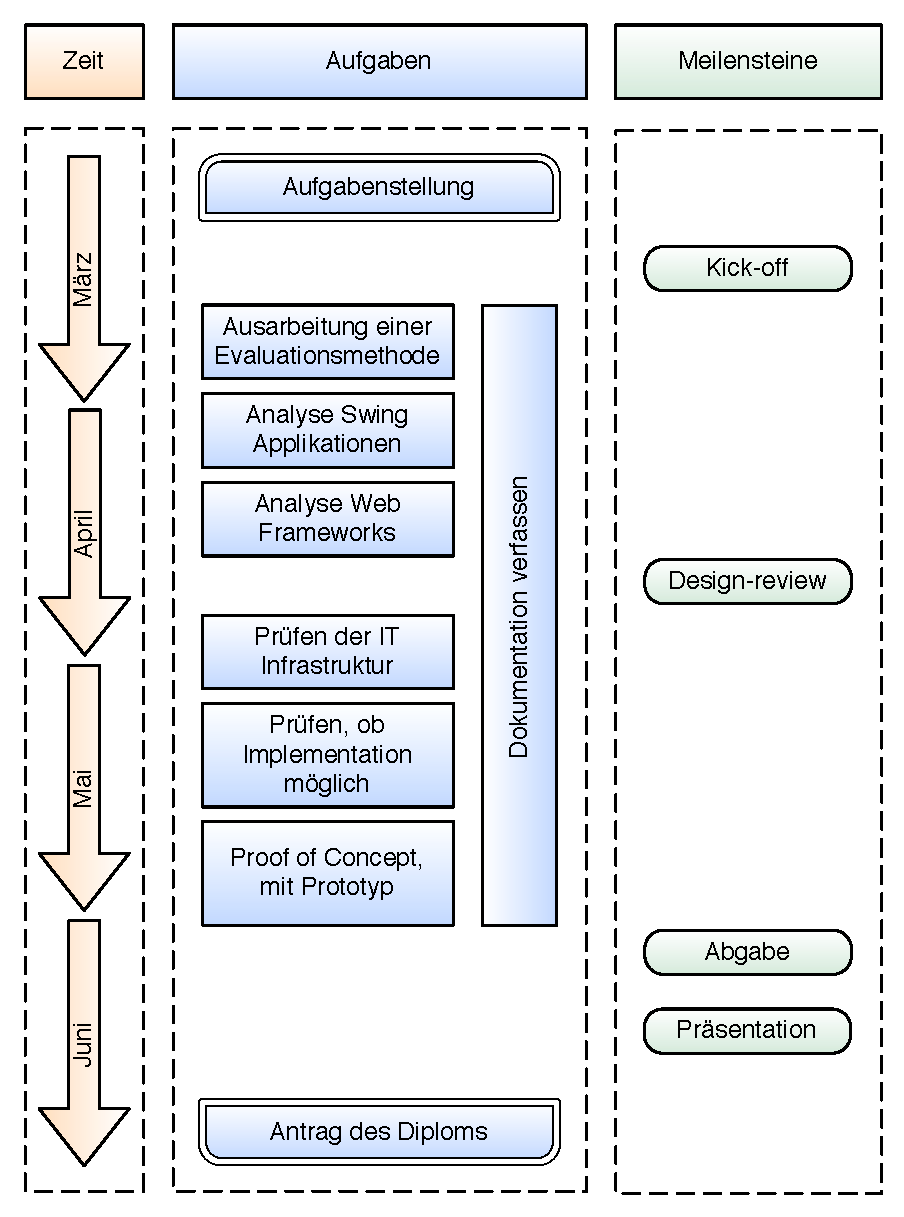
\includegraphics[width=0.85\textwidth]{./image/grobplanung.pdf}
      \caption{Chronologischer Ablauf der Diplomarbeit}
      \label{img:grobplanung}
    \end{center}
  \end{figure}
  
  \subsubsection{Präsentationen}
  
  Gemäss \cite{KillerPresentation} Slide 37f. braucht man für eine Stunde
  Präsentationszeit mindestens eine Vorbereitungszeit von 30 Stunden. Somit kann
  man das linear herunter brechen auf eine Stunde Vorbereitungszeit pro zwei
  Minuten Präsentationszeit. Die Planung ist in der Tabelle
  \ref{tab:presentationPlaning} ersichtlich.
  \newline
  
  \begin{table}[ht]
    \sffamily 
    \begin{center}
      \begin{tabular}{p{9cm}rr}
        \toprule
        \textbf{Arbeitspaket} & \textbf{Geplant} & \textbf{Effektiv} \\
        \midrule
        Kick-off Präsentation ca. 5 Minuten &
        2.5 h &
        4.0 h\\
        Design-review Präsentation ca. 10 Minuten &
        5.0 h &
        \ldots\\
        Schlusspräsentation ca. 20 Minuten &
        10.0 h &
        \ldots\\
        Prototyp Demo ca. 5 Minuten &
        2.5 h &
        \ldots\\
        \bottomrule
        Total &
        20.0 h &
        \ldots\\
        \bottomrule
      \end{tabular}
      \caption{Geplante Zeit für Präsentationen}
      \label{tab:presentationPlaning}
    \end{center}
  \end{table}
  
  \subsubsection{Gestellte Aufgaben gemäss Aufgabenstellung}
  
  Die einzelnen Aufgaben sollen in deren Teilaufgaben unterteilt werden. Die
  Planung ist in der Tabelle \ref{tab:aufgabenPlaning} auf Seite
  \pageref{tab:aufgabenPlaning} ersichtlich.
  
  \subsubsection{Abzugebende Dokumente}
  
  Gemäss den Bestimmungen für die Diplomarbeit, siehe \cite{hsz_reglement} S. 3,
  müssen einige Dokumente erstellt und abgegeben werden. Die Planung ist in der
  Tabelle \ref{tab:documentationPlaning} ersichtlich.
  \newline
  
  \begin{table}[htb]
    \sffamily 
    \begin{center}
      \begin{tabular}{p{9cm}rr}
        \toprule
        \textbf{Arbeitspaket} & \textbf{Geplant} & \textbf{Effektiv} \\
        \midrule
        Bericht in \LaTeX{} aufsetzen &
        10.0 h &
        \ldots\\
        Bericht in \LaTeX{} verfassen &
        60.0 h &
        \ldots\\
        Poster für die Diplomausstellung im A0 Format &
        16.0 h &
        \ldots\\
        Zusammenfassung à zwei A4-Seiten &
        8.0 h &
        \ldots\\
        \bottomrule
        Total &
        94.0 h &
        \ldots\\
        \bottomrule
      \end{tabular}
      \caption{Geplante Zeit für Dokumentation}
      \label{tab:documentationPlaning}
    \end{center}
  \end{table}
  
  \begin{table}[p]
    \sffamily 
    \begin{center}
      \begin{tabular}{lp{7cm}rr}
        \toprule
        \textbf{Aufgabe} & \textbf{Arbeitspaket} & \textbf{Geplant} &
        \textbf{Effektiv}\\

        \midrule
        Au1 &
        Research zu Analyseverfahren von Java Swing Applikationen &
        8.0 h &
        \ldots\\
        &
        Definition des Analyseverfahrens &
        4.0 h &
        \ldots\\
        &
        Analyse von drei Java Swing Applikationen, à 4 Stunden &
        12.0 h &
        \ldots\\

        \midrule
        Au2 &
        Research zu Java Swing Komponenten &
        4.0 h &
        \ldots\\
        &
        Analyse von drei Java Swing Applikationen, à 2 Stunden &
        6.0 h &
        \ldots\\

        \midrule
        Au3 &
        Research zu Evaluationsverfahren im Bereich von Java Web Frameworks &
        12.0 h &
        \ldots\\
        &
        Definition des Evaluationsverfahrens &
        8.0 h &
        \ldots\\
        &
        Evaluation von vier Java Web Frameworks, à 5 Stunden &
        20.0 h &
        \ldots\\

        \midrule
        Au4 &
        Analyse der IT Architektur der ZKB &
        8.0 h &
        \ldots\\
        &
        Prüfen ob die Integration möglich ist bei vier Java Web Frameworks, à
        2.5 Stunden &
        10.0 h &
        \ldots\\
        
        \midrule
        Au5 &
        Analyse der Komponenten von vier Java Web Frameworks und prüfen ob die
        Implementation möglich ist, à 3 Stunden &
        12.0 h &
        \ldots\\
        
        \midrule
        Au6 &
        Anforderungen an den Prototyp definieren &
        8.0 h &
        \ldots\\
        &
        Testfälle für den Prototyp definieren &
        8.0 h &
        \ldots\\
        &
        Umsetzung des Prototypen &
        20.0 h &
        \ldots\\
        &
        Empfehlung eines Java Web Frameworks &
        4.0 h &
        \ldots\\
        \bottomrule
        &
        Total &
        144.0 h &
        \ldots\\
        \bottomrule
      \end{tabular}
      \caption{Geplante Zeit für gestellte Aufgaben}
      \label{tab:aufgabenPlaning}
    \end{center}
  \end{table}
  
  
  \subsubsection{Fachbetreuung durch den Dozenten}
  
  Gemäss den Bestimmungen für die Diplomarbeit, siehe \cite{hsz_reglement} S. 2,
  stehen dem Diplomand zehn Stunden Betreuungszeit durch den Dozenten zur
  Verfügung. Die Planung ist in der Tabelle \ref{tab:observationPlaning}
  ersichtlich.
  \newline
  
  \begin{table}[htb]
    \sffamily 
    \begin{center}
      \begin{tabular}{p{9cm}rr}
        \toprule
        \textbf{Arbeitspaket} & \textbf{Geplant} & \textbf{Effektiv} \\
        \midrule
        Kick-off Meeting &
        1.0 h &
        1.0 h\\
        Design-review Meeting &
        1.0 h &
        \ldots\\
        Schlusspräsentation &
        1.0 h &
        \ldots\\
        Ausserterminliche Betreeuungszeit &
        7.0 h &
        \ldots\\
        \bottomrule
        Total &
        10.0 h &
        \ldots\\
        \bottomrule
      \end{tabular}
      \caption{Geplante Zeit für Betreuung}
      \label{tab:observationPlaning}
    \end{center}
  \end{table}
  
  \subsubsection{Administrative Aufgaben}
  
  Unter administrative Aufgaben fallen Tätigkeiten wie die Planung von Terminen,
  das Druckenlassen der Dokumentation, die Kommunikation mit der Schulleitung
  und dem Dozenten, usw. Auf Grund meiner Erfahrung mit Projekten, macht das in
  etwa fünf Prozent des gesamten Aufwandes aus.
  \newline
  
  \begin{table}[htb]
    \sffamily 
    \begin{center}
      \begin{tabular}{p{9cm}rr}
        \toprule
        \textbf{Arbeitspaket} & \textbf{Geplant} & \textbf{Effektiv} \\
        \midrule
        Planung von Terminen &
        2.0 h &
        \ldots\\
        Druckenlassen der Dokumentation &
        4.0 h &
        \ldots\\
        Kommunikation mit der Schulleitung und dem Dozenten &
        2.5 h &
        \ldots\\
        Übrige administrative Aufgaben &
        5.0 h &
        \ldots\\
        \bottomrule
        Total &
        13.5 h &
        \ldots\\
        \bottomrule
      \end{tabular}
      \caption{Geplante Zeit für administrative Aufgaben}
      \label{tab:administrationPlaning}
    \end{center}
  \end{table}
  
  \section{Arbeitsschritte}
  
  Alle vorgenommenen Arbeitsschritte werden in einem Wiki für die
  Nachvollziehbarkeit protokolliert. Das Wiki ist im Internet öffentlich
  zugänglich unter der \ac{URL}:
  \newline
  
  \url{https://github.com/sushicutta/Diplomarbeit/wiki/Arbeitsprotokoll}
  \newline
  
  \noindent
  Zusätzliche Informationen zum Ablauf der Diplomarbeit werden ebenfalls im Wiki
  erfasst und sind unter der \ac{URL} ersichtlich:
  \newline
  
  \url{https://github.com/sushicutta/Diplomarbeit/wiki/}
  
  \section{Meilensteine}
  
  Die Meilensteine entsprechen dem vorgegebenen Ablauf einer Diplomarbeit aus
  dem \ac{EBS}\footnote{\url{https://ebs.hsz-t.ch/}}. Die Projekt Termine wurden
  alle gemäss Reglement eingehalten, siehe Tabelle \ref{tab:milestones}.
  \newline
  
  \begin{table}[htb]
    \sffamily 
    \begin{center}
      \begin{tabular}{lp{7cm}ll}
        \toprule
        \textbf{Datum} & \textbf{Meilenstein} & \textbf{Ort} \\
        \midrule
        14. März 2011 &
        Die Aufgabenstellung zur Diplomarbeit wurde eingereicht &
        \ac{EBS}\\
        15. März 2011 &
        Freigabe der Diplomarbeit &
        \ac{EBS}\\
        21. März 2011 &
        Inhaltliches Kick-off Meeting &
        Panter llc\\
        13. April 2011 &
        Offizielles Kick-off Meeting &
        \ac{HSZ-T}\\
        04. Mai 2011 &
        Design-Review Meeting &
        \ac{HSZ-T}\\
        15. Juni 2011 &
        Abgabe der Dokumentation &
        \ac{HSZ-T}\\
        29. Juni. 2011 &
        Schlusspräsentation &
        \ac{HSZ-T}\\
        \bottomrule
      \end{tabular}
      \caption{Projekt Meilensteine}
      \label{tab:milestones}
    \end{center}
  \end{table}
 
  \section{Erreichte Ziele}
  
  Es wurden alle Ziele gemäss den erwarteten Resultaten der Aufgabenstellung
  erreicht. Die einzelnen Punkte sind hier aufgeführt, siehe Tabelle
  \ref{tab:erreichteZiele} auf Seite \pageref{tab:erreichteZiele}.
  \newline
  
  \begin{table}[p]
    \sffamily 
    \begin{center}
      \begin{tabular}{lp{9cm}ll}
        \toprule
        \textbf{Resultat} & \textbf{Ziel} & \textbf{Stand} \\
        \midrule
        \ref{itm:Resultat-01} &
          Es soll eine Liste der erkannten GUI Paradigmen vorliegen. &
          erreicht\\
        \ref{itm:Resultat-02} &
          Es soll eine Liste der verwendeten Swingkomponenten vorliegen. &
          erreicht\\
        \ref{itm:Resultat-03} &
          Es soll eine Rangliste der vier Java Web Frameworks, in der Anordnung
          entsprechend ihrer Eignung, vorliegen. &
          offen\\
        \ref{itm:Resultat-04} &
          Es sollen die Java Web Frameworks aufgelistet werden, welche für
          einen Einsatz in der IT Infrastruktur der Zürcher Kantonalbank in
          Frage kommen. &
          erreicht\\
        \ref{itm:Resultat-05} &
          Es sollen die Java Web Frameworks aufgelistet werden, welche die
          notwendigen Swingkomponenten und GUI Paradigmen unterstützen. &
          offen\\
        \ref{itm:Resultat-06} &
          Ein lauffähiger Prototyp. &
          offen\\
        \ref{itm:Resultat-07} &
          Es soll eine Empfehlung eines Java Web Frameworks, für den möglichen
          Einsatz in der Zürcher Kantonalbank, ausgesprochen werden. &
          offen\\
        \bottomrule
      \end{tabular}
      \caption{Übersicht der erreichten Ziele}
      \label{tab:erreichteZiele}
    \end{center}
  \end{table}

  \cleardoublepage
   
  % ===========================================================================
  % Kapitel 18 Anforderungen nach AgileLearn beginns here
  % ===========================================================================  
    
  \chapter{18 Anforderungen an Web Frameworks nach
  AgileLearn}\label{chapter:18AnforderungenNachAgileLearn}
 
    Folgende Anforderungen stammen aus dem Dokument ``\begin{itshape}18
  Anforderungen an Webframeworks -
  OpenDoc\end{itshape}'', siehe \cite{AnforderungenAnWebframeworks}, und werden
  hier zusammengefasst.
  
  \section{Auflistung der Anforderungen}
  
  Die Anforderungen sind hier aufgelistet und mit einer ID in der Form
  Soll\}-\{Laufnummer\} versehen, da die Anforderungen als Soll-Kriterien für
  die Evaluation der Java Web Frameworks dienen.
  
  \begin{description}

    \item[Soll-01 - Zugriffskontrolle
    (Authentifizierung/Authorisation/Rollenverwaltung)\label{itm:Soll-01}]

    Ein Webframework sollte EntwicklerInnen verschiedene Mechanismen
    bereitstellen, um die Anwendung vor fremden und unerlaubten Zugriff schützen
    zu können.

    Authentifizierung/Autorisierung: Üblicherweise werden im Vorfeld Rollen für
    verschiedenen Gruppen festgelegt. Das Ziel einer sicheren Webanwendung ist
    es, bestimmte Bereiche einer Seite abzusichern und die Rechte aller
    Benutzer je nach Rolle einzuschränken. Anhand der Rolle wird deren
    Benutzer für die festgelegten Bereiche autorisiert.

    Vertraulichkeit / Verschlüsselung: Sensible Daten, wie Passwörter und
    Personendaten, müssen vor dem Zugriff und der Kenntnisnahme von Dritten
    geschützt werden. Hierfür werden die Daten während der Übertragung
    verschlüsselt. Für eine sichere Datenübertragung werden meist
    Verschlüsselungsprotokolle wie SSL (Secure Sockets Layer), sowie dessen
    Nachfolger TLS (Transport Layer Security) eingesetzt. Diese gelten als
    relativ sicher und sind bei Transaktionen bei einer Bank unverzichtbar.

    \item[Soll-02 - Form-Validierung\label{itm:Soll-02}]
    Das Verarbeiten von Formularen bzw. die Handhabung von Benutzereingaben und
    -aktionen gehört zu den täglichen Aufgaben der Webentwicklung. Die Logik
    für server- und clientseitiges Validieren ist im Idealfall nur einmal
    implementiert.

    Server-Side Validation: Das Webframework soll die Mögichkeit bieten,
    eingegebene Daten einfach zu überprüfen. Dabei soll für jede Eigenschaft
    eines Datenmodells (Model) ein Wertebereich definierbar sein, zusätzlich
    soll geprüft werden, ob die Eingabe erforderlich ist. Die Programmierlogik
    soll minimal sein. Nach dem Senden der Daten wird alles überprüft und ggf.
    entsprechende Fehlermeldungen zurückgegeben.

    Client-Side Validation: Das Webframework soll wenn möglich schon auf dem
    Client validieren. Wenn möglich, sollen die Daten gleich bei oder kurz nach
    der Eingabe überprüft werden, wobei die Logik auf dem Server implementiert
    ist. Beispiel: Ist der Anmeldename schon vergeben. Dadurch werden
    Serverressourcen gespart und der Benutzer hat ein direktes Feedback.

    \item[Soll-03 - Modulare Architektur\label{itm:Soll-03}]

    Eine Webanwendung stellt ein Zusammenspiel verschiedenster
    Internettechnologien dar, die wiederum hinsichtlich ihrer Entwicklung einem
    stetigen Wandel unterliegen. Die Herausforderung für die Entwickler ist es,
    die Entwicklung der Technologien im Auge zu behalten um gegebenenfalls
    Neuheiten oder Änderungen im System anzupassen. Eine Webanwendung sollte
    daher in all ihren Bestandteilen möglichst wartbar bleiben.

    \item[Soll-04 - Schnittstellen und Webservices\label{itm:Soll-04}]

    Interoperabilität beschreibt den Austausch von Informationen verschiedener
    Softwaresysteme. Es gibt verschiedene Technologien, mit denen ein
    Informationsaustausch umgesetzt werden kann - REST, SOAP und RPC sind am
    weitesten verbreitet. Das Webframework sollte Mechanismen und Funktionen
    zur Umsetzung von Schnittstellen bereitstellen.
    
    \item[Soll-05 - MVC-Entwurfsmuster\label{itm:Soll-05}]
    Besonders im Web hat sich das Model-View-Controller Entwurfsmuster als
    quasi Standard-Architekturmuster für Webanwendungen etabliert und hält
    daher Einzug bei den meisten Webframeworks. Es dient zur Strukturierung der
    Software in drei Einheiten. Das Model (Datenmodell) enthält die
    Geschäftslogik - die Informationen die dargestellt werden. Der Controller
    (Steuerung) ist die Schnittstelle zwischen der View und dem Datenmodell. Er
    nimmt Benutzeraktionen entgegen (z.B. Formulardaten) und leitet sie an ein
    bestimmtes Datenmodell weiter. Der Controller führt dann Operationen wie
    speichern, ändern und löschen auf dem Datenmodell (besser gesagt dem
    Objekt) aus. Die View ist die Präsentationsschicht und stellt die Daten
    dar, die es vom Controller entgegennimmt. Jedoch sollte eine View nicht
    ohne einen Controller neue Objekte erzeugen oder speichern (Trennung von
    Logik und Darstellung). Mit dem MVC-Entwurfsmuster können u.a.
    ProgrammiererInnen und DesignerInnen während der Entwicklung unabhängig
    voneinander arbeiten.

    \item[Soll-06 - Testing\label{itm:Soll-06}]

    Testing ist mit test-driven development (TDD), vor allem in der agilen
    Softwareentwicklung, ein fester Bestandteil während der Projektentwicklung.
    Vor der Implementierung überprüft der Programmierer, mittels Unit-Tests, 
    konsequent das Verhalten jeglicher Komponenten. Gerade kritische Prozesse
    und Transaktionen (zum Beispiel eine Banküberweisung) sollten ausgiebig
    getestet werden. Das Webframework soll die Möglichkeit von Unit-Tests
    bieten.

    \item[Soll-07 - Internationalisierung und Lokalisierung\label{itm:Soll-07}]

    Viele Webanwendungen richten sich mittlerweile an ein internationales
    Publikum. Dank der Offenheit und der weiten Verbreitung des Internets lassen
    sich dadurch sehr einfach neue Zielgruppen (BenutzerInnen) erschließen.
    Jedoch gilt es, einige Vorraussetzungen und Besonderheiten bei der
    Internationalisierung von Webanwendungen zu beachten. Zunächst müssen
    sämtliche Texte übersetzt und möglicherweise in neue Datenbanken ausgelagert
    werden. Hierbei ist zu berücksichtigen, dass es länderspezifische
    Zeichensätze, Zahlen, Datum und Währungswerte gibt. Hinzu kommt, dass unter
    Umständen auch spezielle Grafiken neu erstellt werden müssen.
    
    \item[Soll-08 - Object Relational Mapping (ORM)\label{itm:Soll-08}]
    Die meisten Webframeworks unterstützen das objektorientierte
    Programmierparadigma. Im Zusammenhang mit relationalen Datenbanken kommt es
    allerdings zu grundlegenden Problemen, weil der Zustand und das Verhalten
    eines Objekts nicht in einer relationalen Datenbank gespeichert werden
    kann. Dies ist auf die beiden widersprüchlichen Konzepte von
    objektorientierter Programmierung (OOP) und relationalen
    Datenbankmanagementsystemen (RDMS) zurückzuführen. Im Gegensatz zu
    objektorientierten Datenbanken, werden beim ORM die Tabellen aus der
    Datenbank als Klassen abgebildet (gemappt). Durch die Klassenabbildung wird
    für den/die ProgrammiererIn wieder die gewohnte OOP-Umgebung geschaffen.
    Wenn ein Objekt erstellt oder geändert wird, ist der Mapper verantwortlich,
    um diese Informationen in der Datenbank zu speichern und auch ggfs. wieder
    zu löschen. ORM bildet somit eine Schnittstelle zwischen OOP und
    relationalen Datenbanken.

    Unterstützung von Transaktionen: Bei der Speicherung von Informationen in
    mehreren Datenbanktabellen muss sicher gestellt sein, dass entweder alle
    oder keine Informationen gespeichert werden.

    \item[Soll-09 - Scaffolding / Rapid Prototyping\label{itm:Soll-09}]

    Mit Scaffolding ist das automatische Generien von den sogenannten CRUD-Pages
    (Create, Read, Update, Delete) gemeint.

    Scaffolding und das dadurch verstandene Rapid Prototyping ist ein
    wesentlicher Aspekt der agilen Softwareentwicklung (zum Beispiel in
    Verwendung mit der Scrum-Methodik). Gerade zu Beginn eines Projekts eignet
    sich das Rapid Prototyping, da Änderungen in den Models umgehend in die
    Views eingebunden werden können.

    \item[Soll-10 - Caching\label{itm:Soll-10}]

    Neben der Übertragunsgeschwindigkeit gibt es eine Menge anderer Faktoren,
    die für eine leistungsstarke Webanwendung entscheidend sind. Ein Aspekt ist
    das Caching - das Zwischenspeichern von Daten, die häufig verwendet bzw.
    aufgerufen werden.

    Das Caching kann meist auf verschiedenen Ebenen implementiert werden: Auf
    dem Client, auf dem Webserver und auf der Datenbankebene. Dabei soll das
    Webframework diese Mechanismen unterstützen und es ermöglichen, diese
    einfach zu aktivieren und zu kalibrieren.  

    \item[Soll-11 - View-Engine\label{itm:Soll-11}]

    View Engines werden eingesetzt, um das Arbeiten mit den Views zu
    erleichtern. Sie unterstützen vor allem das Templating - das Erstellen von
    Vorlagen. Durch typisierte Views wird eine Webanwendung robuster, weil
    weniger fehleranfällig; durch partial Views (oft auch nur als partials
    bezeichnet) werden einzelne Elemente oder Bereiche der Benutzeroberfläche
    wiederverwendbar gemacht. Diese Vorlagen können von mehreren Views genutzt
    werden. Dadurch wird deutlich weniger redundanter Code erstellt. Dies ist
    ein wichtiger Aspekt in Bezug auf das Don’t repeat yourself (DRY) Prinzip.

    \item[Soll-12 - Dokumentation\label{itm:Soll-12}]

    Eine Webanwendung ist aus Entwicklersicht eine Zusammenfassung
    verschiedenster Technologien (Webframeworks, Bibliotheken, Schnittstellen).
    Über das Application Programming Interface (API) haben Programmierer Zugriff
    auf die verfügbaren Funktionen. Nicht selten erstreckt sich die
    Dokumentation einer API über mehrere hundert Seiten. Für Programmierer ist
    es daher von enormer Bedeutung, dass die Bibliotheken gut strukturiert und
    verständlich beschrieben sind. Schlecht oder gar nicht dokumentierte
    Technologien erhöhen die Fehlerquote und sind oft ausschlaggebend für einen
    nicht flüssigen Workflow.

    \item[Soll-13 - Community\label{itm:Soll-13}]

    Die beteiligten Personen in den Foren, Mailing-Listen oder Wikis bilden im
    Zusammenhang mit Webframeworks die Community. Es findet dabei ein
    Wissensaustausch statt, der weit über die standard-Dokumentation hinaus
    geht. Die Nutzer helfen sich gegenseitig bei Problemen und Fehlern und oft
    hinterlassen sie mit ihren Einträgen wiederum einen Lösungsansatz, der
    zukünftig von anderen wieder aufgegriffen werden kann. Es ist daher 
    wichtig, dass den Anwendern eine Möglichkeit geboten wird, sich
    auszutauschen, gemeinsam Fehlermeldungen zu deuten und Lösungsansätze zu
    entwickeln.

    \item[Soll-14 - IDE-Unterstützung\label{itm:Soll-14}]

    In der Softwareentwicklung ist die IDE das Basiswerkzeug für die
    Programmierer. Die Entwicklungsumgebung stellt den Entwicklern verschiedene
    Komponenten zur Verfügung, wie Editor, Compiler, Linker oder Debugger.
    Hinzu kommen mit Syntaxhighlighting, Refactoring und Code-Formatierung
    weitere wichtige Funktionen, die die Entwickler in vielerlei Hinsicht enorm
    unterstützen.

    \item[Soll-15 - Kosten für Entwicklungswerkzeuge\label{itm:Soll-15}]

    Je nach verfügbaren finanziellen Mitteln spielen die Kosten von
    Entwicklungswerkzeugen und Technologien durchaus eine Rolle. Bei beiden
    Faktoren hat man meist die Wahl zwischen kostenlosen (OpenSource) und
    kommerziellen Produkten. Je nach Webanwendung müssen somit Lizenzgebühren
    für die Entwicklungswerkzeuge, Server zum Ausführen der Anwendung und
    Datenbankserver berücksichtigt werden. Dabei ist es wichtig die richtige
    Mischung verschiedener Komponenten zu finden.
  
    \item[Soll-16 - Eignung für agile Entwicklung\label{itm:Soll-16}]

    Die herkömmlichen Methoden der Software-Entwicklung werden heute oft durch
    neue agile Methoden, wie Extreme Programming oder Scrum abgelöst. Sie
    fokussieren auf das Wesentliche und stehen für deutlich mehr Flexibilität in
    der Entwicklungsphase als konventionelle Methoden. Verschiedene Technologien
    unterstützen die agilen Methoden. Refactoring, Testing spielt dabei eine
    wichtige Rolle und soll unterstützt werden.

    \item[Soll-17 - Lernkurve für EntwicklerInnen\label{itm:Soll-17}]

    Zur Umsetzung einer komplexen Webanwendung wird den Entwicklern ein Wissen
    über verschiedenste Bereiche der Softwareentwicklung abverlangt.
    Glücklicherweise gibt es für die Webentwicklung keinen einheitlichen
    Standard, der festlegt, wie eine Webanwendung entwickelt werden muss. Das
    Internet bietet für jeden Bereich eine Auswahl unterschiedlicher
    Technologien an. Daher müssen vor der Entwicklung mehrere Entscheidungen
    getroffen werden - hinsichtlich Programmiersprache, Javascript-Framework
    oder Datenbankserver. Es werden daher oft Technologien gewählt, die leicht
    zu erlernen und verstehen sind.

    Wichtig ist, dass man einen schnellen Einstieg bekommt und Erfolge bald
    sichtbar werden, um die Motivation der Entwickler zu erhöhen.

    \item[Soll-18 - AJAX-Unterstützung\label{itm:Soll-18}]

    Durch das Aufkommen von Javascript-Bibliotheken wie jQuery und Prototype
    haben sich vollkommen neue Möglichkeiten eröffnet mit Javascript auf dem
    Client zu arbeiten und mit AJAX wurde die Kommunikation zwischen Server und
    Client im Web revolutioniert. Die direkte Unterstützung eines
    Javascript-Frameworks ist für ein Webframework sinnvoll und erwünscht.

    Darüber hinaus sollte die unterstützte Bibliothek lose gekoppelt sein, und
    damit austauschbar. Sogenanntes unobtrusive Javascript, bei dem auch bei
    abgeschaltetem Javascript die Anwendung funktioniert, ist auch eine Anforderung.
  \end{description}

  \cleardoublepage
   
  % ===========================================================================
  % Kapitel Grundsätze der ZKB IT-Architektur beginns here
  % ===========================================================================  
    
  \chapter{Grundsätze der ZKB
  IT-Architektur}\label{chapter:GrundsaetzeDerZkbItArchitektur}
 
    Die Grundsätze sind aus dem \begin{itshape}Handbuch der
  IT-Architektur\end{itshape}, siehe \cite{ZkbHandbuchDerItArchitektur}, der
  \ac{ZKB} entnommen.
  
  \section{Auflistung der Grundsätze}
  
  Die Grundsätze sind hier aufgelistet und mit einer ID in der Form
  \{KO\}-\{Laufnummer\} versehen, da die Grundsätze als KO-Kriterien für die
  Evaluation der Java Web Frameworks dienen.

  \begin{description}

    % Kapitel 2.2.2, N-Tier Applikationen, Seite 20
    \item[KO-01\label{itm:KO-01}]
    \footnote{\cite{ZkbHandbuchDerItArchitektur} Kapitel 2.2.2 -
    \begin{itshape}N-Tier Applikationen\end{itshape}, Seite 20}
    Applikationen sollen als N-Tier Applikationen designed und
    implementiert werden.

    % Kapitel 2.2.10, Objektorientierung, Seite 22
    \item[KO-02\label{itm:KO-02}]
    \footnote{\cite{ZkbHandbuchDerItArchitektur} Kapitel 2.2.10 -
    \begin{itshape}Objektorientierung\end{itshape}, Seite 22}
    \ac{OO} soll innerhalb der Informatik für Neuentwicklungen
    durchgängig angewandt werden.

    % Kapitel 3.3, Mehrsprachigkeit, Seite 36
    \item[KO-03\label{itm:KO-03}]
    \footnote{\cite{ZkbHandbuchDerItArchitektur} Kapitel 3.3 -
    \begin{itshape}Mehrsprachigkeit\end{itshape}, Seite 36}
    Eine neue Applikation (oder eine neue Komponente einer
    bestehenden Applikation) ist mehrsprachfähig zu realisieren.

    % Kapitel 3.3, Mehrsprachigkeit, Seite 37
    \item[KO-04\label{itm:KO-04}]
    \footnote{\cite{ZkbHandbuchDerItArchitektur} Kapitel 3.3 -
    \begin{itshape}Mehrsprachigkeit\end{itshape}, Seite 37}
    Neue Applikationen sind Unicode-fähig zu realisieren.

    % Kapitel 3.9.1, Skalierbarkeit / Ausfallsicherheit / Perfomance
    % Seite 49
    \item[KO-05\label{itm:KO-05}]
    \footnote{\cite{ZkbHandbuchDerItArchitektur} Kapitel 3.9.1 -
    \begin{itshape}Skalierbarkeit / Ausfallsicherheit / Perfomance\end{itshape},
    Seite 49}
    Eine Applikation muss in mehreren Instanzen lauffähig sein.

    % Kapitel 4.4.1, User Interface, Seite 55
    \item[KO-06\label{itm:KO-06}]
    \footnote{\cite{ZkbHandbuchDerItArchitektur} Kapitel 4.4.1 -
    \begin{itshape}User Interface\end{itshape}, Seite 55}
    Der ZKB GUI Style Guide ist in allen ZKB IT-Projekten anzuwenden.
    
    % Kapitel 5.2, Verwendung der Zentralen Server Infrastruktur ZSI, Seite 57
    \item[KO-07\label{itm:KO-07}]
    \footnote{\cite{ZkbHandbuchDerItArchitektur} Kapitel 5.2 -
    \begin{itshape}Verwendung der Zentralen Server Infrastruktur
    ZSI\end{itshape}, Seite 57}
    Die \ac{ZSI} ist als Server-Plattform für Applikationen, welche Windows-,
    Unix-, Linux-basierte Server einsetzen, zu verwenden.
    
    % Kapitel 9.2, Java RMI, Seite 71
    \item[KO-08\label{itm:KO-08}]
    \footnote{\cite{ZkbHandbuchDerItArchitektur} Kapitel 9.2 -
    \begin{itshape}Java RMI\end{itshape}, Seite 71}
    RMI kann für reine Java-Anwendungen eingesetzt werden.
    
    % Kapitel 12.2.1, Einsatz von Frameworks, Seite 140
    \item[KO-09\label{itm:KO-09}]
    \footnote{\cite{ZkbHandbuchDerItArchitektur} Kapitel 12.2.1 -
    \begin{itshape}Einsatz von Frameworks\end{itshape}, Seite 140}
    Für Java-Applikationen (Internet, Extranet und Intranet) wird das
    ZIP-Framework eingesetzt.
    
    % Kapitel 12.3.5, Client-/Server-Schemata von Internet-Applikationen,
    % Seite 141
    \item[KO-10\label{itm:KO-10}]
    \footnote{\cite{ZkbHandbuchDerItArchitektur} Kapitel 12.3.5 -
    \begin{itshape}Client-/Server-Schemata von Internet-Applikationen\end{itshape}, Seite 141}
    Die Validierung und Plausibilisierung der Eingaben erfolgt immer
    abschliessend auf dem bankseitigen Applikations-Server. Es ist aber
    durchaus möglich, dass sich auf der Client-Seite eine Logik zur Überprüfung
    und Validierung der Eingaben für den Benutzerkomfort befindet.
    
    % Kapitel 12.3.5, Client-/Server-Schemata von Internet-Applikationen,
    % Seite 141
    \item[KO-11\label{itm:KO-11}]
    \footnote{\cite{ZkbHandbuchDerItArchitektur} Kapitel 12.3.5 -
    \begin{itshape}Client-/Server-Schemata von Internet-Applikationen\end{itshape}, Seite 141}
    Die Business-Logik in einer Internet-Applikation ist so auszulegen, dass
    diese von verschiedenen Präsentations-Logiken im Rahmen von Ultra-Thin- und
    Thin-Client-Applikationen genutzt werden kann.
    
    % Kapitel 12.3.6.1, Browser-Abhängigkeiten, Seite 142
    \item[KO-12\label{itm:KO-12}]
    \footnote{\cite{ZkbHandbuchDerItArchitektur} Kapitel 12.3.6.1 -
    \begin{itshape}Browser-Abhängigkeiten\end{itshape}, Seite 142}
    Die Internet-Applikationen der ZKB werden nicht mit Browser-Abhängigkeiten
    versehen und orientieren sich an den neutralen Standards der W3C-Komission.
    
    % Kapitel 12.3.6.2, Session-Mechanismus, Seite 142
    \item[KO-13\label{itm:KO-13}]
    \footnote{\cite{ZkbHandbuchDerItArchitektur} Kapitel 12.3.6.2 -
    \begin{itshape}Session-Mechanismus\end{itshape}, Seite 142}
    Für Ultra-Thin-Client-Applikationen wird als Session-Mechanismus die
    Cookie- oder die URL-Rewriting-Methode angewendet.
    
    % Kapitel 12.3.6.4, Einfache Internet-Applikationen, Seite 143
    \item[KO-14\label{itm:KO-14}]
    \footnote{\cite{ZkbHandbuchDerItArchitektur} Kapitel 12.3.6.4 -
    \begin{itshape}Einfache Internet-Applikationen\end{itshape}, Seite 143}
    Einfache Internet-Applikationen mit dem Schwerpunkt Information können
    ausschliesslich Java Server Pages verwenden.
    
    % Kapitel 12.3.6.5, Komplexe Internet-Applikationen, Seite 143
    \item[KO-15\label{itm:KO-15}]
    \footnote{\cite{ZkbHandbuchDerItArchitektur} Kapitel 12.3.6.5 -
    \begin{itshape}Komplexe Internet-Applikationen\end{itshape}, Seite 143}
    Komplexe Internet-Applikationen verwenden eine Kombination von Java Server
    Pages und mindestens einem Servlet als Dispatcher-Mechanismus.
    
    % Kapitel 12.3.6.6, Verwendung von JavaScript beziehungsweise ECMAScript
    % Seite 143
    \item[KO-16\label{itm:KO-16}]
    \footnote{\cite{ZkbHandbuchDerItArchitektur} Kapitel 12.3.6.6 -
    \begin{itshape}Verwendung von JavaScript beziehungsweise
    ECMAScript\end{itshape}, Seite 143}
    Die Internet-Applikationen funktionieren auch eingeschränkt, ohne dass die
    Skript-Funktion im Browser aktiviert ist.
    
    % Kapitel 12.3.6.7, Einstz von ActiveX und Cookies, Seite 143
    \item[KO-17\label{itm:KO-17}]
    \footnote{\cite{ZkbHandbuchDerItArchitektur} Kapitel 12.3.6.6 -
    \begin{itshape}Verwendung von JavaScript beziehungsweise
    ECMAScript\end{itshape}, Seite 143}
    ActiveX wird wegen der Möglichkeit für direkte Zugriffe auf das
    Betriebssystem nicht eingesetzt.
    
    % Kapitel 12.3.6.8, Applets, Seite 144
    \item[KO-18\label{itm:KO-18}]
    \footnote{\cite{ZkbHandbuchDerItArchitektur} Kapitel 12.3.6.8 -
    \begin{itshape}Applets\end{itshape}, Seite 144}
    Es werden keine neuen Applikationen als Java Applets entwickelt. Der
    Einsatz von Applets beschränkt sich auf einfache Funktionen wie Börsen-
    oder News-Ticker.
    
    % Kapitel 12.3.6.9, Browser-Plugins, Seite 144
    \item[KO-19\label{itm:KO-19}]
    \footnote{\cite{ZkbHandbuchDerItArchitektur} Kapitel 12.3.6.9 -
    \begin{itshape}Browser-Plugins\end{itshape}, Seite 144}
    Internet-Applikation werden ohne Plugins entwickelt.
    
    % Kapitel 12.3.7, Client-Technologien, Seite 144
    \item[KO-20\label{itm:KO-20}]
    \footnote{\cite{ZkbHandbuchDerItArchitektur} Kapitel 12.3.7 -
    \begin{itshape}Client-Technologien\end{itshape}, Seite 144}
    Für Ultra Thin Clients bzw. Browser-basierende Applikationen muss das
    aktuelle, Struts-basierende HTML-Client-Framework der ZKB Internet
    Plattform verwendet werden.
    
    % Kapitel 12.3.8, Layering von Internet-Applikationen, Seite 145
    \item[KO-21\label{itm:KO-21}]
    \footnote{\cite{ZkbHandbuchDerItArchitektur} Kapitel 12.3.8 -
    \begin{itshape}Layering von Internet-Applikationen\end{itshape}, Seite 145}
    Neue Internet- und Extranet-Applikationen müssen sich an das Layering
    gemäss nachfolgender Grafik halten. Für Intranet-Applikationen ist die
    Validator-Komponente fakultativ.
    
    % Kapitel 12.3.8, Layering von Internet-Applikationen, Seite 146
    \item[KO-22\label{itm:KO-22}]
    \footnote{\cite{ZkbHandbuchDerItArchitektur} Kapitel 12.3.8 -
    \begin{itshape}Layering von Internet-Applikationen\end{itshape}, Seite 146}
    Eine Applikation muss ohne Änderung von der Intranet-Anwendung zur Extra-
    oder Internet-Applikation gemacht werden können. Es geschieht dies
    lediglich durch das Vorschalten der Validator-Komponente.
    
    % Kapitel 12.3.10.2, Web Server, Seite 146
    \item[KO-23\label{itm:KO-23}]
    \footnote{\cite{ZkbHandbuchDerItArchitektur} Kapitel 12.3.10.2 -
    \begin{itshape}Web Server\end{itshape}, Seite 146}
    Der ZKB Standard-Web-Server ist der Apache HTTP-Server.
    
    % Kapitel 12.4.2, Architektur beim Einsatz von Application-Servern,
    % Seite 147
    \item[KO-24\label{itm:KO-24}]
    \footnote{\cite{ZkbHandbuchDerItArchitektur} Kapitel 12.4.2 -
    \begin{itshape}Architektur beim Einsatz von
    Application-Servern\end{itshape}, Seite 147}
    Der Application-Server wird als die integrierte technische Middleware für
    die Unterstützung von Java Server Pages (JSP), Servlets, Enterprise Java
    Beans (EJB) und der sicheren Kommunikation zwischen Client und Server
    eingesetzt.
    
    % Kapitel 12.4.2, Architektur beim Einsatz von Application-Servern,
    % Seite 148
    \item[KO-25\label{itm:KO-25}]
    \footnote{\cite{ZkbHandbuchDerItArchitektur} Kapitel 12.4.2 -
    \begin{itshape}Architektur beim Einsatz von
    Application-Servern\end{itshape}, Seite 148}
    Der ZKB Standard-J2EE-Application-Server ist der JBoss Application Server.
    
    % Kapitel 12.4.2, Architektur beim Einsatz von Application-Servern,
    % Seite 148
    \item[KO-26\label{itm:KO-26}]
    \footnote{\cite{ZkbHandbuchDerItArchitektur} Kapitel 12.4.2 -
    \begin{itshape}Architektur beim Einsatz von
    Application-Servern\end{itshape}, Seite 148}
    Der J2EE-Application-Server wird in der \ac{ZSI} eingesetzt.
    
    % Kapitel 12.4.2, Architektur beim Einsatz von Application-Servern,
    % Seite 148
    \item[KO-27\label{itm:KO-27}]
    \footnote{\cite{ZkbHandbuchDerItArchitektur} Kapitel 12.4.2 -
    \begin{itshape}Architektur beim Einsatz von
    Application-Servern\end{itshape}, Seite 148}
    Die Serverplattform für den Einsatz von Web-Application-Servern für
    Internet-/Intranet-/Extranet-Applikationen ist Linux.
    
    % Kapitel 12.4.2, Architektur beim Einsatz von Application-Servern,
    % Seite 150
    \item[KO-28\label{itm:KO-28}]
    \footnote{\cite{ZkbHandbuchDerItArchitektur} Kapitel 12.4.2 -
    \begin{itshape}Architektur beim Einsatz von
    Application-Servern\end{itshape}, Seite 150}
    Die technischen Services wie Session Management, Load Balancing,
    Transaction Management und Instance Pooling werden vom J2EE Application
    Server zur Verfügung gestellt.
    
    % Kapitel 12.4.3, Einsatz von Enterprise Java Beans, Seite 150
    \item[KO-29\label{itm:KO-29}]
    \footnote{\cite{ZkbHandbuchDerItArchitektur} Kapitel 12.4.3 -
    \begin{itshape}Einsatz von Enterprise Java Beans\end{itshape}, Seite 150}
    Das Muster JSP/Servlets mit EJBs ist anzuwenden, wenn die Applikation eine
    umfangreiche, komplexe Business-Logik aufweist, die Business-Logik
    wiederverwendbar sein soll, mehrere unterschiedliche Clients (Browser
    (Ultra-Thin-)(HTML), Thin-(Java), Mobile, …) mit einer Business Logik
    bedient werden müssen, hohe Anforderungen an die Skalierbarkeit gestellt
    werden und ein lange Lebenszyklus der Applikation erwartet wird.
    
    % Kapitel 12.4.3, Einsatz von Enterprise Java Beans, Seite 150
    \item[KO-30\label{itm:KO-30}]
    \footnote{\cite{ZkbHandbuchDerItArchitektur} Kapitel 12.4.3 -
    \begin{itshape}Einsatz von Enterprise Java Beans\end{itshape}, Seite 150}
    Das Muster JSP/Servlets ohne EJBs ist anzuwenden, wenn die Applikation eine
    einfache Business-Logik aufweist, nur einen Client, zum Beispiel ein
    Browser (Ultra-Thin-)-Interface unterstützt, niedrige Anforderungen an die
    Skalierbarkeit stellt und nur eine vergleichsweise kurzer Lebenszyklus der
    Applikation erwartet wird.
    
    % Kapitel 12.9.2, Standards, Seite 171
    \item[KO-31\label{itm:KO-31}]
    \footnote{\cite{ZkbHandbuchDerItArchitektur} Kapitel 12.9.2 -
    \begin{itshape}Standards\end{itshape}, Seite 171}
    In der ZKB werden folgende Standards für Web Services eingesetzt: SOAP,
    WSDL, W3C X Schema (XSD, WXS).
    
    % Kapitel 13.1, Client/Server-Konzept, Seite 175
    \item[KO-32\label{itm:KO-32}]
    \footnote{\cite{ZkbHandbuchDerItArchitektur} Kapitel 13.1 -
    \begin{itshape}Client/Server-Konzept\end{itshape}, Seite 175}
    Alle Neuentwicklungen sind konsequent in Client-/Server-Komponenten
    aufzuteilen.
    
    % Kapitel 13.2, Anwendungsstruktur (MVC/Model, View, Controller), Seite 175
    \item[KO-33\label{itm:KO-33}]
    \footnote{\cite{ZkbHandbuchDerItArchitektur} Kapitel 13.2 -
    \begin{itshape}Anwendungsstruktur (MVC/Model, View,
    Controller)\end{itshape}, Seite 175}
    Die gewünschte Isolation der Systemteile wird durch eine Anwendungsstruktur
    mit Trennung in Model (Verarbeitung, Datenhaltung), View
    (Benutzeroberfläche) und Controller (Organisation, Ereignisvermittlung)
    erreicht.
    
    % Kapitel 13.9.7.2, Allgemeine Grundsätze, Seite 189
    \item[KO-34\label{itm:KO-34}]
    \footnote{\cite{ZkbHandbuchDerItArchitektur} Kapitel 13.9.7.2 -
    \begin{itshape}Allgemeine Grundsätze\end{itshape}, Seite 189}
    Jede Applikation ist dafür verantwortlich, dass diejenigen Daten, für die
    sie den Lead hat, validiert sind.
    
    % Kapitel 13.9.7.2, Allgemeine Grundsätze, Seite 189
    \item[KO-35\label{itm:KO-35}]
    \footnote{\cite{ZkbHandbuchDerItArchitektur} Kapitel 13.9.7.2 -
    \begin{itshape}Allgemeine Grundsätze\end{itshape}, Seite 189}
    Jede Applikation benutzt Datenvalidierung um sicherzustellen, dass sie die
    erhaltenen Daten verarbeiten kann und dass ihr Betrieb nicht gefährdet ist
    (Stabilität / Verfügbarkeit).
    
    % Kapitel 13.9.7.3.1, Datenvalidierung an der Benutzersczhnittstelle
    % Seite 191
    \item[KO-36\label{itm:KO-36}]
    \footnote{\cite{ZkbHandbuchDerItArchitektur} Kapitel 13.9.7.3.1 -
    \begin{itshape}Datenvalidierung an der Benutzersczhnittstelle\end{itshape},
    Seite 191}
    Benutzereingaben werden so früh wie möglich validiert.
    
    % Kapitel 13.10, Programmiersprachen und Entwicklungsumgebungen
    % Seite 192
    \item[KO-37\label{itm:KO-37}]
    \footnote{\cite{ZkbHandbuchDerItArchitektur} Kapitel 13.10 -
    \begin{itshape}Programmiersprachen und Entwicklungsumgebungen\end{itshape},
    Seite 192}
    Für die Entwicklung neuer Applikationen und beim neuen Design bestehender
    Applikationen wird Java eingesetzt.
    
    % Kapitel 13.10.4.8, Zusätzliche Java Klassenbibliotheken, Seite 195
    \item[KO-38\label{itm:KO-38}]
    \footnote{\cite{ZkbHandbuchDerItArchitektur} Kapitel 13.10.4.8 -
    \begin{itshape}Zusätzliche Java Klassenbibliotheken\end{itshape}, Seite 195}
    Zusätzliche Java-Klassenbibliotheken, also solche, die nicht im JDK
    enthalten sind, werden nur in begründeten Ausnahmen eingesetzt.
    Normalerweise müssen solche Bibliotheken dem 100\%-Pure-Java-Grundsatz
    entsprechen. Ausnahmen können systemnahe Funktionen für Security und
    dergleichen sein.
    
    % Kapitel 13.11, Einsatz von .NET-basierten Applikationen, Seite 196
    \item[KO-39\label{itm:KO-39}]
    \footnote{\cite{ZkbHandbuchDerItArchitektur} Kapitel 13.11 -
    \begin{itshape}Einsatz von .NET-basierten Applikationen\end{itshape}, Seite
    196}
    .NET-basierte Applikationen werden in der ZKB Informatik nicht entwickelt
    oder zur Entwicklung in Auftrag gegeben ausser Kleinapplikationen der
    Kategorie „Office“.
    
    % Kapitel 13.13, Einsatz von Open Source Software, Seite 206
    \item[KO-40\label{itm:KO-40}]
    \footnote{\cite{ZkbHandbuchDerItArchitektur} Kapitel 13.13 -
    \begin{itshape}Einsatz von Open Source Software\end{itshape}, Seite 206}
    Die Nutzung von Open Source Software ist erlaubt.
    
    % Kapitel 13.13, Einsatz von Open Source Software, Seite 206
    \item[KO-41\label{itm:KO-41}]
    \footnote{\cite{ZkbHandbuchDerItArchitektur} Kapitel 13.13 -
    \begin{itshape}Einsatz von Open Source Software\end{itshape}, Seite 206}
    Open Source Software unterliegt denselben Kriterien wie kommerzielle
    Software. Sie muss evaluiert, registriert, homologiert, intern supported
    und gepflegt werden.    
    
    % Kapitel 13.13.1, Kriterien für die Evaluation von Open Source
    % Software, Seite 207
    \item[KO-42\label{itm:KO-42}]
    \footnote{\cite{ZkbHandbuchDerItArchitektur} Kapitel 13.13.1 -
    \begin{itshape}Kriterien für die Evaluation von Open Source
    Software\end{itshape}, Seite 207}
    Produktiv eingesetzte Open Source Software muss durch angemessene
    Informationsquellen unterstützt sein (Newsgroups, Mailinglists,
    FAQ-Listen, WebSites, User Groups).    
    
    % Kapitel 13.13.1, Kriterien für die Evaluation von Open Source
    % Software, Seite 207
    \item[KO-43\label{itm:KO-43}]
    \footnote{\cite{ZkbHandbuchDerItArchitektur} Kapitel 14.14.1 -
    \begin{itshape}Kriterien für die Evaluation von Open Source
    Software\end{itshape}, Seite 207}
    Die Weiterentwicklung von produktiv eingesetzter Open Source Software
    ausserhalb der ZKB muss öffentlich einsehbar sein und aktiv verfolgt werden
    können.
    
    % Kapitel 13.13.1, Kriterien für die Evaluation von Open Source
    % Software, Seite 207
    \item[KO-44\label{itm:KO-44}]
    \footnote{\cite{ZkbHandbuchDerItArchitektur} Kapitel 13.13.1 -
    \begin{itshape}Kriterien für die Evaluation von Open Source
    Software\end{itshape}, Seite 207}
    Die Lizenzbedingungen einer Open Source Software müssen vor dem Einsatz
    geprüft werden und von der Zürcher Kantonalbank akzeptiert werden können.
  \end{description}

  \cleardoublepage

  % ===========================================================================
  % Protokolle beginns here
  % ===========================================================================
 
  % ===========================================================================
  % Kick-off Protokoll beginns here
  % ===========================================================================
 
  \chapter{Kick-off Protokoll}\label{chapter:KickOffProtokoll}

    \section{Anwesende Personen}
    
  \begin{table}[ht]
    \begin{center}
      \begin{tabular}{rlc}
        \toprule
        Funktion & Person & Anwesend\\
        \midrule
        Student & Roman Würsch & Ja\\
        Auftraggeber & Bernhard Mäder, ZKB & Nein\\
        Projektbetreuer & Beat Seeliger & Ja\\
        Experte & --- & Nein\\
        Vertreter Studiengang Informatik & Olaf Stern & Ja\\
        \bottomrule
      \end{tabular}
      \captionsetup{list=no}
      \caption{Anwesende Personen}
      \label{tab:anwesendePersonen}
    \end{center}
  \end{table}

  \section{Beschlüsse}
  \begin{itemize}
      \item Gemäss Email von Herr Stern vom 17. März 2011
      \begin{itemize}
        \item ``Sie führen in Absprache mit Ihrem Betreuer ein inhaltliches
        Kick-Off durch. Gibt Ihr Betreuer sein OK anschliessend, fahren Sie
        mit der Bearbeitung der Arbeit fort (kein Zeitverlust für Sie).''
        \item ``An dem von Ihnen gebuchten Termin am 13. April führen wir
        ein verkürztes Kick-Off durch, dieses wird auch als das formale
        Kick-Off in EBS eingetragen und protokolliert.''
      \end{itemize} 
      \item Gemäss Email von Herr Stern vom 15. März 2011: Es wurden
      die geforderten Änderungen an der Aufgabenstellung angepasst.
      \item Es soll ein RIA - Framework (z.B. ULC) mit in die Evaluation
      genommen werden.
      \item Es soll ein MVC - Framework (z.B. Struts) mit einbezogen
      werden.
      \item Es werden die Bewertungskriterien für die Bachelor Arbeit verwendet.
      \item Der Zeitplan ist straff, sportlich, sollte aber machbar sein.
  \end{itemize}
  
  \cleardoublepage
  
  % ===========================================================================
  % Design-review  Protokoll beginns here
  % ===========================================================================
   
  \chapter{Design-review Protokoll}\label{chapter:DesignReviewProtokoll}
  
    \section{Anwesende Personen}
    
  \begin{table}[ht]
    \begin{center}
      \begin{tabular}{rlc}
        \toprule
        Funktion & Person & Anwesend\\
        \midrule
        Student & Roman Würsch & Ja\\
        Auftraggeber & Bernhard Mäder, ZKB & Nein\\
        Projektbetreuer & Beat Seeliger & Ja\\
        Experte & --- & Nein\\
        Vertreter Studiengang Informatik & Olaf Stern & Ja\\
        \bottomrule
      \end{tabular}
      \captionsetup{list=no}
      \caption{Anwesende Personen}
      \label{tab:anwesendePersonen}
    \end{center}
  \end{table}

  \section{Beschlüsse}
  \begin{itemize}
      \item Gemäss Email von Herr Stern vom 17. März 2011
      \begin{itemize}
        \item ``Sie führen in Absprache mit Ihrem Betreuer ein inhaltliches
        Kick-Off durch. Gibt Ihr Betreuer sein OK anschliessend, fahren Sie
        mit der Bearbeitung der Arbeit fort (kein Zeitverlust für Sie).''
        \item ``An dem von Ihnen gebuchten Termin am 13. April führen wir
        ein verkürztes Kick-Off durch, dieses wird auch als das formale
        Kick-Off in EBS eingetragen und protokolliert.''
      \end{itemize} 
      \item Gemäss Email von Herr Stern vom 15. März 2011: Es wurden
      die geforderten Änderungen an der Aufgabenstellung angepasst.
      \item Es soll ein RIA - Framework (z.B. ULC) mit in die Evaluation
      genommen werden.
      \item Es soll ein MVC - Framework (z.B. Struts) mit einbezogen
      werden.
      \item Es werden die Bewertungskriterien für die Bachelor Arbeit verwendet.
      \item Der Zeitplan ist straff, sportlich, sollte aber machbar sein.
  \end{itemize}
  
  \cleardoublepage
  
  % ===========================================================================
  % Abkürzungsverzeichnis beginns here
  % ===========================================================================
  
  \chapter{Abkürzungsverzeichnis}\label{chapter:Abkuerzungsverzeichnis}

  \begin{multicols}{2}

\begin{acronym}[RDBMS]
  \setlength{\itemsep}{-\parsep}
  \acro{AHP}{Analytic Hierarchy Process}
  \acro{API}{Application Programming Interface}
  \acro{Ajax}{Asynchronous JavaScript and XML}
  \acro{BRE}{Business Request Exchange}
  \acro{CORBA}{Common Object Request Broker Architecture}
  \acro{CSS}{Cascading Style Sheets}
  \acro{EBS}{Einschreibe- und Bewertungssystem der HSZ-T}
  \acro{EDT}{Event Dispatch Thread}
  \acro{FAQ}{Frequently Asked Questions}
  \acro{GUI}{Grafische Benutzeroberfläche}
  \acro{GWT}{Google Web Toolkit}
  \acro{HSZ-T}{Hochschule für Technik Zürich}
  \acro{HTML}{Hypertext Markup Language}
  \acro{HTTP}{Hypertext Transfer Protocol}
  \acro{HTTPS}{Hypertext Transfer Protocol Secure}
  \acro{IDE}{Integrierte Entwicklungsumgebung}
  \acro{JDBC}{Java Database Connectivity}
  \acro{JFC}{Java Foundation Classes}
  \acro{JRE}{Java Runtime Environment}
  \acro{JSP}{JavaServer Pages}
  \acro{MOM}{Message oriented Middleware}
  \acro{MVC}{Model View Controller}
  \acro{MVP}{Model View Presenter}
  \acro{NWA}{Nutzwertanalyse}
  \acro{OO}{Objektorientierung}
  \acro{ORM}{Object Relational Mapping}
  \acro{PDF}{Portable Document Format}
  \acro{PNG}{Portable Network Graphics}
  \acro{RDBMS}{Relational Database Management System}
  \acro{RIA}{Rich Internet Application}   
  \acro{RMI}{Remote Method Invocation}
  \acro{SOAP}{Simple Object Access Protocol}
  \acro{SVG}{Scalable Vector Graphics}
  \acro{UI}{User Interface}
  \acro{UML}{Unified Modeling Language}
  \acro{URL}{Uniform Resource Locator}
  \acro{ZIP}{ZKB Internet Plattform}
  \acro{ZKB}{Zürcher Kantonalbank}
  \acro{ZSI}{Zentrale Server Infrastruktur}
\end{acronym}

\end{multicols}
  
  \cleardoublepage
  
  % ===========================================================================
  % Abbildungsverzeichnis beginns here
  % ===========================================================================
  
  \listoffigures
  
  \cleardoublepage
  
  % ===========================================================================
  % Tabellenverzeichnis beginns here
  % ===========================================================================
  
  \listoftables
  
  \cleardoublepage

  % ===========================================================================
  % Quellcodeverzeichnis beginns here
  % ===========================================================================
    
  \renewcommand{\lstlistlistingname}{Listingverzeichnis}
  
  \lstlistoflistings
  
  \cleardoublepage
  
  % ===========================================================================
  % Literaturverzeichnis beginns here
  % ===========================================================================
  
  % verwendet alpha
  \bibliographystyle{alpha}
  % verwendet Literaturverzeichnis.bib
  % \renewcommand\bibname{Literaturverzeichnis} % Titel überschreiben
  
  \bibliography{Literaturverzeichnis}\label{chapter:Literaturverzeichnis}
  
  \cleardoublepage

\end{document}